%some-literature review


In the last few decades, several scientists have modeled the dynamics and ecological impact of marine aggregates~\cite{jackson_aggregation_1998, kiorboe_mechanisms_2002}. 
Their effects on bacterial transport~\cite{jackson_simulation_1989} and algal bloom~\cite{jackson_model_1990} have been described in models that use simplified descriptions of the aggregates' settling speeds. Moreover, accumulation of aggregates in thin layers where the ambient fluid is stratified has been reported~\cite{macintyre_accumulation_1995, alldredge_occurrence_2002} and more recently modeled experimentally~\cite{prairie_delayed_2013}, analytically~\cite{camassa_retention_2013}, and computationally~\cite{panah_simulations_2017}. 
Understanding marine aggregate's formation, settling speed, and persistence of these thin layers is ecologically important. 
Therefore, in this chapter, we discuss the dynamics of settling marine aggregates in a density-stratified fluid. 
%--------------------------------------------------------
\section{Governing Equations}
In this chapter, instead of constant density $\rho$, as in Chapter 2, we suppose that the background fluid density varies linearly in the vertical direction,
\begin{equation}
\rho_{bg}(z) =  \rho_0 \left(1 - \gamma z \right),
\label{eq_rho_bg}
\end{equation}
where $\rho_0$ is the fluid density where the aggregate's center of mass is located at rest initially and $\gamma > 0$ is constant.
Over time, perturbations, $C(\vec{y},t)$, in the fluid density occur due to the settling motion. More specifically, we define $C$ as the concentration difference between the values at initial and time $t$.
From this, we can establish the fluid density variation over time,
\begin{equation}
	\rho(\vec{y},t ) 
	= \rho_{bg}(z) +  \alpha \rho_0 C(\vec{y},t) 
	 = \rho_0 \left( 1 - \gamma z  + \alpha  C(\vec{y},t) \right),
\label{eq_density}
\end{equation}
where the non-zero constant $\alpha$ depends on the type of solute. 
\begin{figure}[ht]
	\begin{center}
	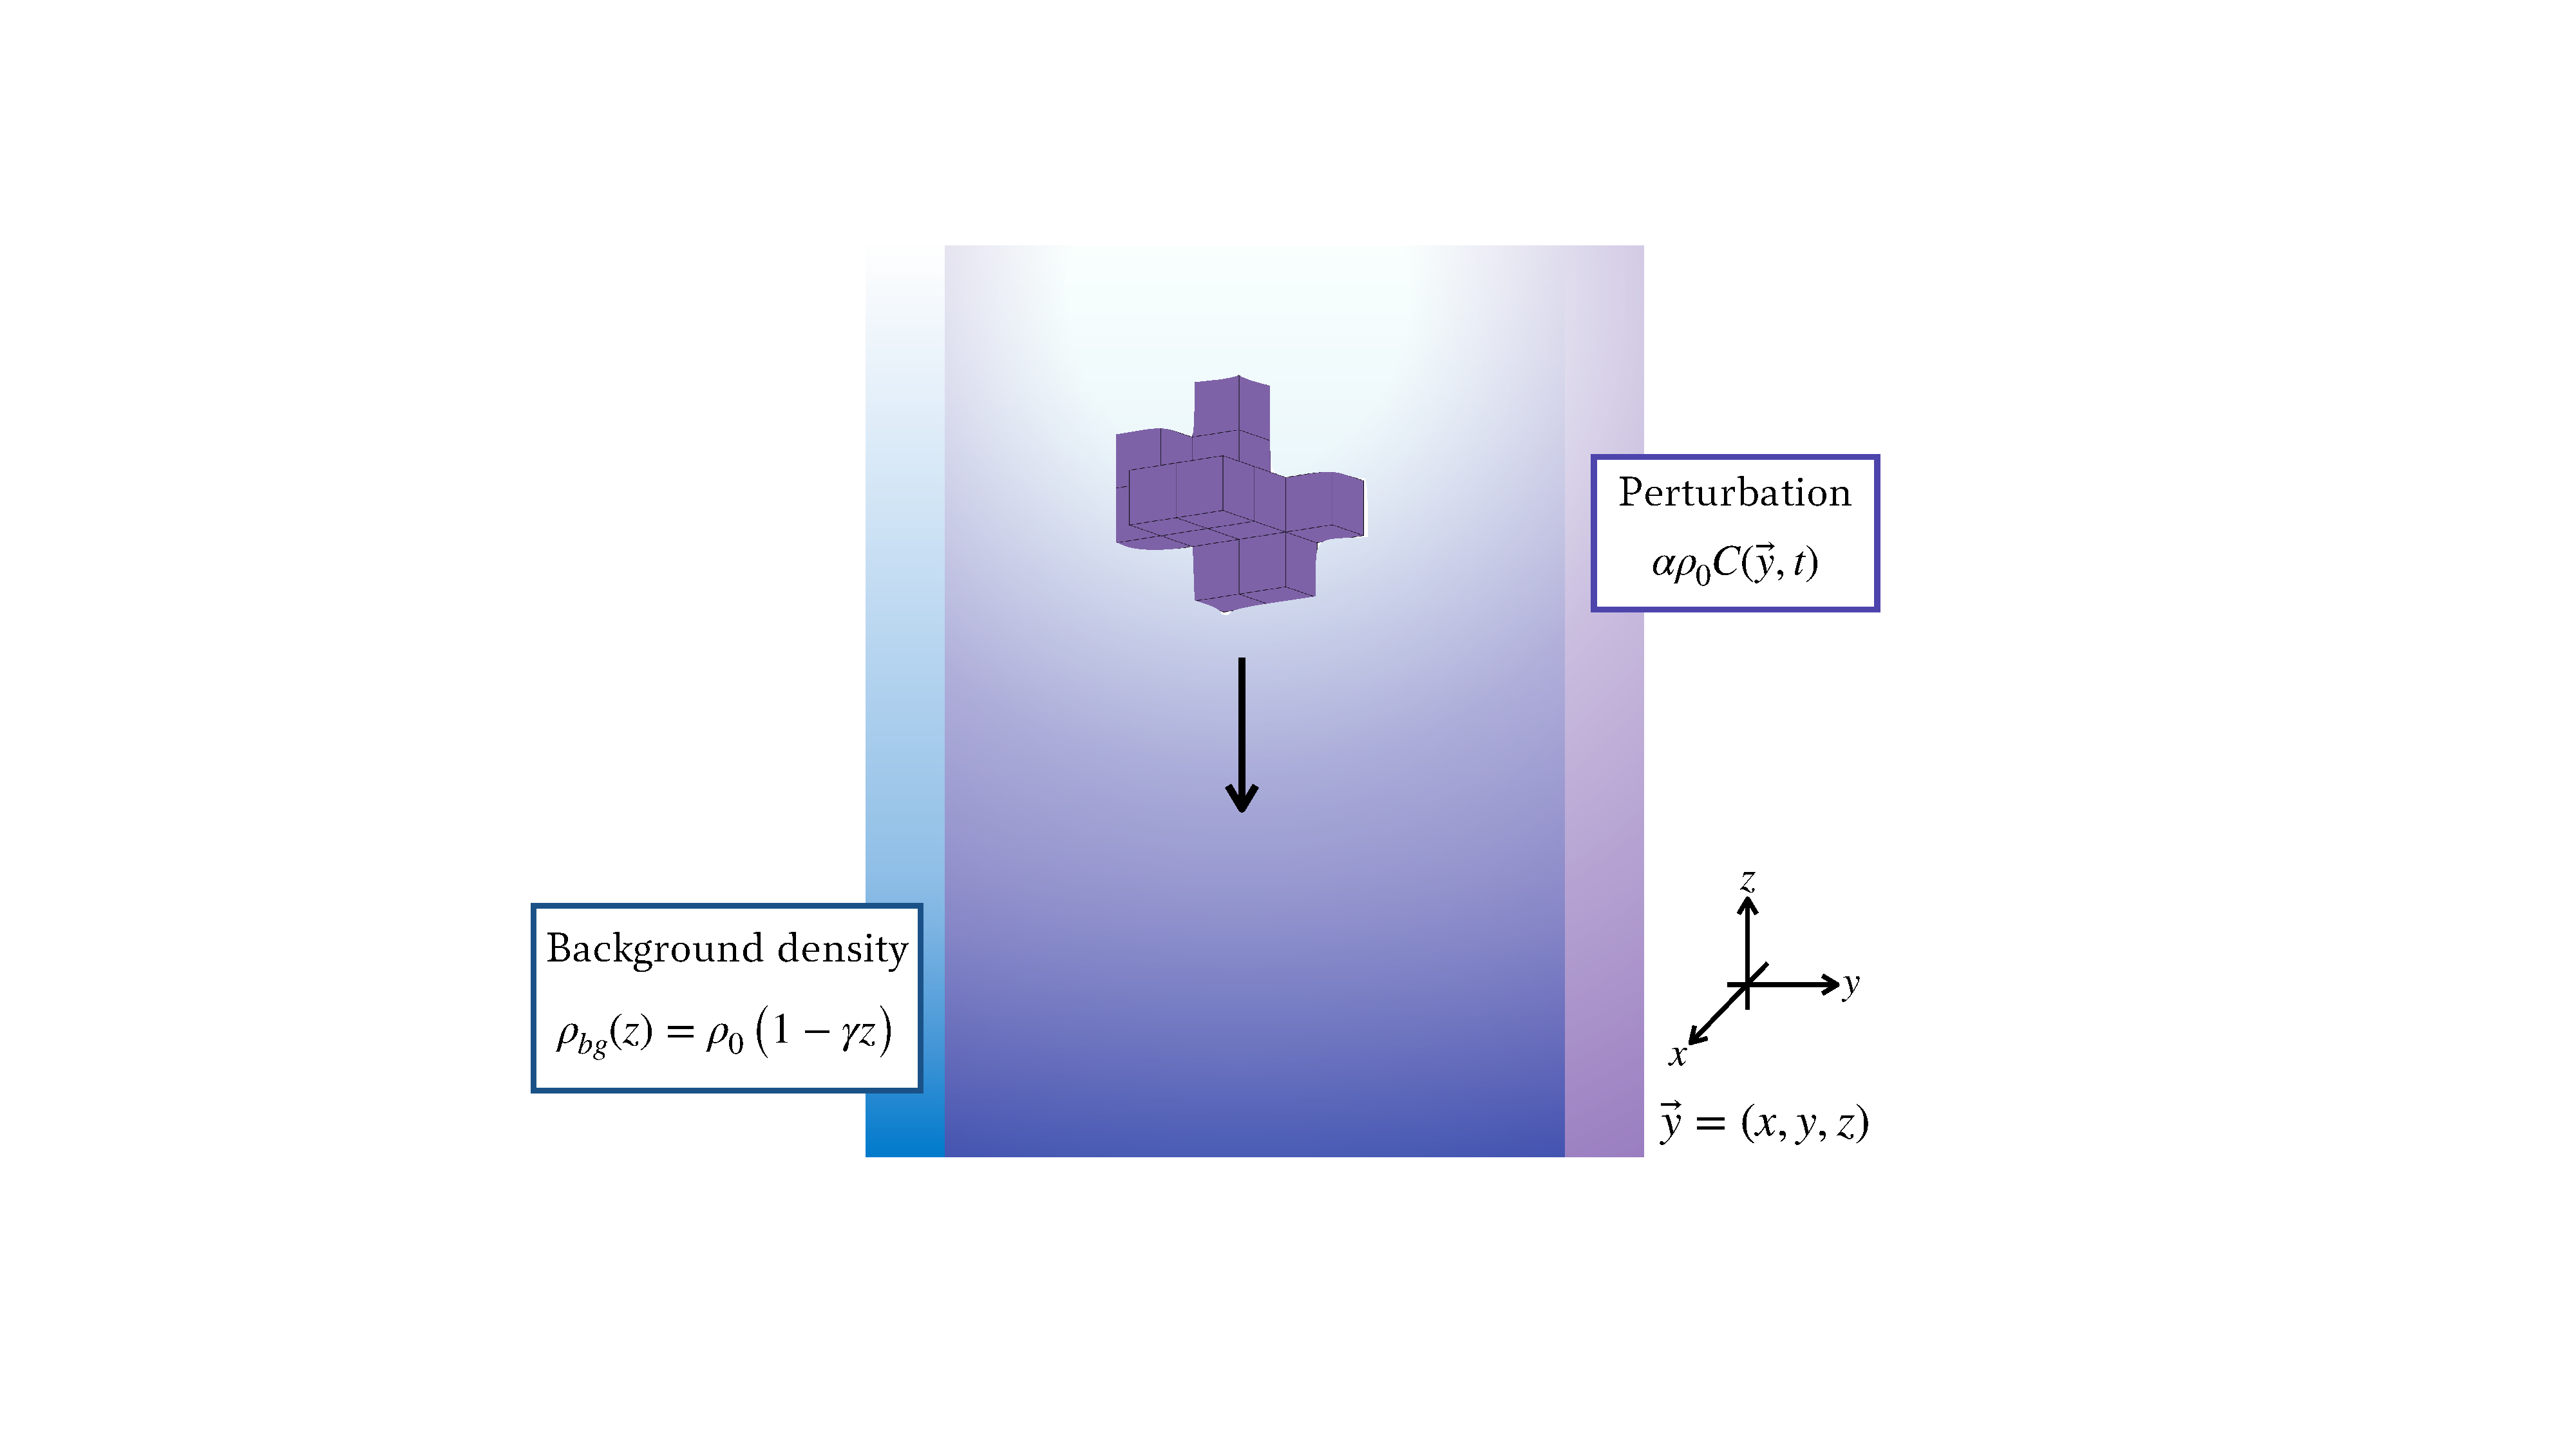
\includegraphics[scale=0.4]{./figures/fig_stratification_schematics}
	\caption{Description of fluid density stratification.}
	\label{fig_stratification_schematics}
	\end{center}
\end{figure}
The non-constant density $\rho(\vec{y},t)$ changes the momentum equation from (\ref{eq_stokes3}) to 
		 \begin{equation}
		\ \tilde{\mu}\nabla^2 \vec{u}(\vec{y})
		- \nabla P_d (\vec{y}) \ + \  
		 \rho_0 \alpha C(\vec{y},t) \vec{g} =0 , 
	\label{eq_extra_C}
	\end{equation}
	where $P_d$ is the dynamic pressure, defined as
\begin{equation}
	P_d (\vec{y})
	 = P (\vec{y}) \ - \int \rho_{bg}(z) g   \textrm{d}z.
	\label{eq_Pd}
\end{equation}
To take the perturbation of the ambient fluid into account, we find a particular solution to the momentum equation (\ref{eq_extra_C}). Once we have it, simple addition to the homogenous solution gives the entire solution due to the linearity of the system. 
\par
% \subsection{Particular solution to Stokes equations with the stratification}
%----------------------------------------------------------------------
To derive a particular solution, we consider the singularly forced Stokes problem~\cite{pozrikidis_boundary_1992},
\begin{equation}
	\ \tilde{\mu} \nabla^2 \vec{u}(\vec{y})
	- \nabla P (\vec{y})
	+\vec{q} \ \delta \left(\vec{x} - \vec{y} \right) =0,
\label{eq_single_stokes}
\end{equation}
where $\vec{q}$ is an arbitrary constant vector, $\vec{x}$ is an arbitrary point in fluid domain, and $\delta$ is the three-dimensional delta function.
The problem (\ref{eq_single_stokes}) 
describes the effect coming from a singular force applied at $\vec{y} = \vec{x}.$
The fundamental solution to equation (\ref{eq_single_stokes}) coupled with the continuity equation (\ref{eq_conserv_mass}) are
\begin{equation}
	\vec{u} (\vec{y}) = \ \frac{1}{8\pi \tilde{\mu}}  \bar{\bar{G \ }}(\vec{x}, \vec{y})
	\cdot  \vec{q}
\label{eq_fund_u}
\end{equation}
\begin{equation}
	P (\vec{y}) = \ \frac{1}{4\pi }  
	\frac{\vec{x} - \vec{y}}{\| \vec{x} - \vec{y}\|^3}
	\cdot  \vec{q},
\label{eq_fund_p}
\end{equation}
where the kernel $\bar{\bar{G \ }}$ is the \textit{Stokeslet}, introduced in Chapter 1, equation (\ref{eq_stokeslet}).
This implies that the solutions (\ref{eq_fund_u}) and (\ref{eq_fund_p}) satisfy equation (\ref{eq_single_stokes}) as
\begin{equation}
	\ \tilde{\mu} \nabla^2 
	\biggl( \frac{1}{8\pi \tilde{\mu}}  \bar{\bar{G \ }}(\vec{x}, \vec{y})
	\cdot  \vec{q} \biggr)
	- \nabla \biggl(\ \frac{1}{4\pi }  
	\frac{\vec{x} - \vec{y}}{\| \vec{x} - \vec{y}\|^3}
	\cdot  \vec{q} \biggr)
	+ \vec{q} \ \delta \left(\vec{x} - \vec{y} \right)
	=0.
\label{eq_single_stokes_sub}
\end{equation}
When we multiply by $ C $ on both sides and integrate the entire equation over the domain, $V(\vec{x})$, we get
\begin{equation}
	\int_{V}
	\biggl[
	\ \tilde{\mu} \nabla^2 
	\biggl( \frac{ \bar{\bar{G \ }}(\vec{x}, \vec{y})
	\cdot  \vec{q}}{8\pi \tilde{\mu}}  \biggr)
	C(\vec{x}, t)
	-
	\nabla \biggl( 
	\frac{(\vec{x} - \vec{y}) \cdot  \vec{q} }{4 \pi \| \vec{x} - \vec{y}\|^3}
	\biggr)
	C(\vec{x}, t)
	+ \vec{q} \ \delta \left(\vec{x} - \vec{y} \right)
	C(\vec{x}, t)
	\biggr]
	\ \textrm{d}V(\vec{x}) = 0 .
\label{eq_single_stokes_sub2}
\end{equation}
Note that the operator $\nabla$ is linear and describes derivatives in $\vec{y}$. We are able to switch the order with the integral operator as follows,
\begin{equation}
	\tilde{\mu} \ \nabla^2 
	\int_{V}
	\biggl( \frac{\bar{\bar{G \ }}(\vec{x}, \vec{y})
	\cdot  \vec{q} }{8\pi \tilde{\mu}}  \biggr)
	C(\vec{x}, t)
	\ \textrm{d}V(\vec{x})
	-
	\nabla 
	\int_{V}
	\biggl(
	\frac{	C(\vec{x}, t)(\vec{x} - \vec{y})\cdot  \vec{q} }{4 \pi \| \vec{x} - \vec{y}\|^3} \biggr)
	\ \textrm{d}V(\vec{x})
	+\vec{q} C(\vec{x}, t) = 0 .
\label{eq_single_stokes_sub3}
\end{equation}
By choosing $\vec{q} = \rho_0 \alpha \vec{g}$, we can find a particular solution to our modified Stokes momentum equation, (\ref{eq_extra_C}),
\begin{equation}
	\vec{u} (\vec{y}) =
	 \frac{\rho_0 \alpha }{8\pi \tilde{\mu}}
	\int_{V}  \bar{\bar{G \ }}(\vec{x}, \vec{y})
	\cdot  C(\vec{x}, t) \vec{g} 
	\ \textrm{d}V(\vec{x}).
\label{eq_fund_soln_unit}
\end{equation}
\begin{equation}
	P(\vec{y}) = 
	\frac{\rho_0 \alpha }{4\pi }  
	\int_{V}
	\frac{\vec{x} - \vec{y}}{\| \vec{x} - \vec{y}\|^3}
	\cdot 
	C(\vec{x}, t) \vec{g} 
	\ \textrm{d}V(\vec{x}).
\label{eq_fund_soln_p}
\end{equation}
The entire velocity solution, thus, becomes
\begin{equation}
	 \vec{u} \left(\vec{y}, t \right) =
	 - \frac{1}{8 \pi \tilde{\mu}} \int_{S}  
		 \vec{f}(\vec{x}) 
		 \cdot \bar{\bar{G \ }} (\vec{x},\vec{y}) 
		 \ \textrm{d}S(\vec{x})
	+ \frac{ \rho_0 \alpha  }{8\pi \tilde{\mu}} \int_V  C \left(\vec{x},  t \right) \vec{g} \cdot 
	\bar{\bar{G \ }}(\vec{x}, \vec{y} ) 
	\ \text{d}V(\vec{x}).
\label{eq_vel_HP}
\end{equation}
As we see, the velocity at a point $\vec{u}$ is now dependent on space and time compared to the homogeneous fluid case, which was time-dependent. We can update the velocity field in time by coupling the solution (\ref{eq_vel_HP}) with the advection-diffusion equation (\ref{eq_ad_diff_nonD}) to model the solute perturbation, $C$.
 
%------------------------------------------------------------------
\subsection{Force balance}
\label{sec:force_balance}
\par
Because the velocity of the aggregate is no longer constant, we need to solve for one.
Specifically, we now need to solve for the translational and angular velocity, $\vec{U}_a$ and $\vec{\Omega}$, respectively, by prescribing the total body force and total torque from the fluid on the aggregate.
To close the system of equations, we prescribe the total drag force, $\vec{F}_o$, and total torque, $\vec{Q}_o$. 

First, we know that the total drag is the sum of stress vectors, $\vec{f}$,
\begin{equation}
	 \vec{F}_o = \int_S \vec{f} (\vec{x}) \ \textrm{d}S 
	= - \int_S \left[ 
	 - \left( P -  \int \rho_{bg}(z) g \ \textrm{d}z \right) \bar{\bar{I \ }} 
	 + \tilde{\mu} \left( \nabla \vec{u} + (\nabla \vec{u})^{T} \right)
	 \right] \cdot \hat{n} \ \textrm{d}S (\vec{y}).
\label{eq_Fo}
\end{equation}
To impose the total drag (\ref{eq_Fo}), we observe the right-hand side of the equation(\ref{eq_Fo}) which includes the buoyancy force. 
As we work in Stokes flow, the net force on the aggregate must be zero, so we have
\begin{equation}
	\vec{F}_o (t)+\vec{F}_g(t) + \vec{F}_b = \vec{0},
\end{equation} 
where the gravity force acting on the aggregate, $\vec{F}_g$, can be expressed as
\begin{equation}
	\vec{F}_g = \rho_a V_a \vec{g}, 
\end{equation}
with aggregate density $\rho_a$ and volume $V_a$. 
To calculate the aggregate density, $\rho_a$, we consider a porosity, $\phi$, that is $ 0 \leq \phi \leq 1$.
 We then define the density of an aggregate as 
\begin{equation}
	\rho_a  = \phi \rho_{f} + (1-\phi) \rho_{s},
	\label{eq_rho_a}
\end{equation}
where $\rho_{f}$ and $\rho_s$ are the density of the liquid and solid portion of the aggregate, respectively. To obtain the liquid portion of the aggregate density, we take an average of the fluid density where the aggregate is located,
\begin{equation}
	\rho_{f}(t) = \frac{1}{V_a}\int_{V_a} \rho(\vec{x}, t) \  \textrm{d}V(\vec{x}))
\end{equation}
We here consider the solid part of the aggregate density as $\rho_s \approx 1400 $kg$/$m$^3.$ 
We also set the porosity to $\phi = 0.95$.
Meanwhile, we find the buoyancy force, $\vec{F}_b$, from the equation (\ref{eq_Fo}),
\begin{equation}
 \vec{F}_b =	  -  \int_S \left( 
	   \int \rho_{bg}(z) g \ \textrm{d}z 
	 \right) \bar{\bar{I \ }}  \cdot
	\hat{n} \ \textrm{d}S (\vec{y}).
\label{eq_Full_Force}
\end{equation}

For the total torque, we use the form (\ref{eq_torquebal}), and set the value to zero,
\begin{equation}
	\vec{Q}_o =\int_S \vec{f}\times (\vec{x} - \vec{x}_{cm}) \ \textrm{d}S =  \vec{0}.
\label{eq_Qo}
\end{equation}
 Note that this does not imply that the aggregate is not rotating. 
%--------------------------------------------------
\subsection{Perturbation variation}
As the aggregate settles, the concentration, and therefore the fluid density, changes
\begin{equation}
	\frac{\partial \rho(\vec{y},t)}{\partial t}
	+ \vec{u}(\vec{y}) \cdot \nabla \rho(\vec{y},t)
	 = D \nabla^2 \rho(\vec{y},t),
\label{eq_AD_rho}
\end{equation}
where $D$ is the diffusion coefficient.
By applying the relationship between fluid density $\rho$ and perturbation $C$ from equation (\ref{eq_density}), we can re-write the equation (\ref{eq_AD_rho}) in terms of $C$, 
\begin{equation}
	\frac{\partial C(\vec{y},t)}{\partial t}
	+ \vec{u}(\vec{y}) \cdot \nabla C(\vec{y},t)
	 = D \nabla^2 C(\vec{y},t)
	 + \frac{\gamma}{\alpha}\vec{u}(\vec{y})  \cdot \hat{k}.
\label{eq_AD_C}
\end{equation}
Note that the advection-diffusion equation for $C$ contains an additional source term that
depends on the vertical component of the fluid velocity.

%------------------------------------------------------------------
\section{Dimensional analysis}
To facilitate further analysis, we non-dimensionalize our new equations. We mainly use the same parameters we introduced in section~\ref{section3}, equations (\ref{eq_nonD}), in addition to the following dimensionless parameters:
\begin{equation}
	C= C_{max} C'
\hspace{7mm}
\rho = \frac{\tilde{\mu}  }{{U_s} R_a}  \rho', 
\end{equation}
In this chapter, the Stokes settling speed $U_s$, defined in equation (\ref{eq_U_s}), becomes
\[
U_s = \frac{g  L^2}{\tilde{\mu}}(\rho_s - \rho_0)(1-\phi),
\] 
since we consider the porosity of an aggregate as (\ref{eq_rho_a}).
% Note that the Reynolds number is approximately 0.03.
 % Here $\rho_a$ is the density of aggregate.
For the scale of the perturbation, $C$, we introduce the maximum density difference of the background density profile in the fluid domain at the initial time, i.e., 
\begin{equation}
C_{max} = 
\frac{1}{\alpha \rho_0}
\left|
\max_{\vec{x}\in V} \left(\rho_{bg}(z)  \right)
\ - \min_{\vec{x} \in V} \left(\rho_{bg}(z)  \right) \right|.
\end{equation}
\par
We first derive the dimensionless modified Stokes momentum equation, using primes to indicate dimensionless variables,
\begin{equation}
	{\nabla'}^2  \vec{u}'(\vec{y})
	= \nabla {P_d}'(\vec{y}) \ - \  
	\frac{\alpha \rho_0  C_{max}}{(\rho_s - \rho_0)(1-\phi)}  C'\left(\vec{y},t \right)   \hat{k},
\label{eq_extra_C_nonD}
\end{equation}
which is then solved for the velocity,
 \begin{align}
		\vec{u}'(\vec{y})
			  & =- \frac{1}{8 \pi} \int_{S'}  
			 \vec{f'}(\vec{x}) 
			 \cdot \bar{\bar{G' \ }} (\vec{x},\vec{y}) 
			 \ \textrm{d}S'(\vec{x})
			 \nonumber \\
& -\frac{ \alpha C_{max}}{8\pi } \frac{\rho_0}{(\rho_s - \rho_0)(1-\phi)} 
\int_{V'} C' \left(\vec{x},  t \right) \hat{k} \cdot 
\bar{\bar{G'  }}(\vec{x}, \vec{y} ) 
\ \text{d}V'(\vec{x})
  \label{eq_vel_all_onS_nonD}
 \end{align}
where $S'$ is the aggregate surface. 
Moreover, the force balance equation (\ref{eq_Full_Force}) becomes
\begin{align}
	 \vec{F'}_o(t)
	 & =
	   %\text{[Body force] + [Buoyancy force]}
	  %= 
	  \frac{1}{\tilde{\mu} U_s R_a} 
	  \left(
	-   \rho_a V_a g \hat{k}
	  +
	   \int_{S} \left( 
	   \int \rho_{bg}(z) g \ \textrm{d}z 
	   \right) \bar{\bar{I \ }}  \cdot
	  \hat{n} \ \textrm{d}S (\vec{x})
	\right).
\label{eq_Full_Force_nonD}
\end{align}

\par
Lastly, the advection-diffusion equation becomes, 
	\begin{equation}
	\frac{\partial C'(\vec{x},t)}{\partial t'}
	+ \vec{u}'(\vec{x}) \cdot \nabla' C'(\vec{x},t)
	 = \frac{1}{\textrm{Pe}} {\nabla'}^2 C'(\vec{x},t)
	 +\frac{\gamma R_a}{ \alpha C_{max}} \vec{u}' \cdot \hat{k},
	\label{eq_AD_nonD}
	\end{equation}
using the velocity field, equation (\ref{eq_vel_all_onS_nonD}), for the advection term.
Note that we discussed the Péclet number with CO$_2$ diffusivity in Chapter (\ref{sec:concentration}) while introducing its definition in equation (\ref{eq_def_Pe}).
In addition, we can find the thermal diffusivity of the ocean, $D_{heat}$~\cite{nayar_thermophysical_2016,sharqawy_thermophysical_2010}: we get a Péclet number of

\begin{align}
	\text{Pe}_{heat} 
	= \frac{U_s R_a }{D_{heat}} 
	\approx \frac{3.8 \times 10^{-4}(\text{m/s}) \times \left(5 \times 10^{-5} \right) (\text{m})}{1.5 \times 10^{-7} (\text{m}^2\text{/s})} \approx 10^{-2},
\end{align} 
and the diffusion effect due to salinity~\cite{wollast_diffusion_1971}, 
\begin{align}
	\text{Pe}_{salt}
	= \frac{U_s R_a }{D_{salt}} 
	\approx \frac{3.8 \times 10^{-4}(\text{m/s}) \times \left(5 \times 10^{-5} \right) (\text{m})}{ 2\times 10^{-9} (\text{m}^2\text{/s})} \approx 9.5.
\end{align}
\par
For the rest of this chapter, we drop the prime for simplicity and use only dimensionless forms. 


%---------------Numerics--------------------------------------
\section{Numerical methods}
%-------------------------------------------------------------
In this section, 
We first consider aggregates drag computation. We derive the simplest form to implement in codes. We then revisit the velocity field calculation in a homogeneous fluid. We briefly introduce the linear system to solve for the aggregate's stress and velocity. Lastly, we present the method to compute the velocity field in a fluid with density, involving a volume integral of the perturbation $C(\vec{x},t)$. Due to the high computational cost, we use the fast multipole method (FMM). We briefly introduce the FMM and its framework for the Stokes kernel.
%subsection--------------------------------------------------------------------

\subsection{Aggregate force balance}
We first recall the force balance equation (\ref{eq_Full_Force}), introduced in section~\ref{sec:force_balance}. To obtain the total drag, there are two types of forces we consider: 1) aggregate's body force, $\vec{F}_g$, and 2) fluid buoyancy force, $\vec{F}_b$. 
The aggregate density, $\rho_a$, of the fluid portion changes over time, which affects its (dimensionless) gravitational body force,
\begin{equation}
	\vec{F}_g = 
	- \frac{1}{\tilde{\mu} U_s R_a} 
	\left( \rho_a V_a g \hat{k}	 \right).
	\label{eq_agg_force_G}
\end{equation}
We also need to track the buoyancy, depending on the aggregate's vertical position,
\begin{align}
	\vec{F}_{b}
	 = \frac{1}{\tilde{\mu} U_s R_a} 
	 \left(
	  \int_{S} \left( 
	  \int \rho_{bg}(z) g \ \textrm{d}z 
	  \right) \bar{\bar{I \ }}  \cdot
	 \hat{n} \ \textrm{d}S (\vec{x})
   \right),
   \label{eq_buoyancy_nonD}
\end{align}
since the surrounding fluid density changes while the aggregate settles.
For further simplicity, we find an antiderivative of the background density,
\begin{equation}
	\mathcal{P}_{bg}(z) =  \int \rho_{bg}(z) g \ \textrm{d}z 
	 = \rho_0 \left( z - \frac{1}{2}\gamma z^2 \right) g,
\end{equation}
by choosing the lower bound of the integral as zero without loss of generality.
In practice, we can easily evaluate the gravitational force (\ref{eq_agg_force_G}). While settling, we compute the fluid density where the aggregate is located. Once we know which grid points are inside the aggregate, simply adding the densities at those points gives us the fluid density portion of the aggregate, which eventually plays a role in updating the $\rho_a$. 
\par
Next, we investigate the buoyancy force (\ref{eq_buoyancy_nonD}) with a single cube case for simplicity. 
We can extend this case to multiple cubes in the same manner by addition. We consider the discretized version of integral (\ref{eq_buoyancy_nonD}), 
\begin{equation}
	\vec{F}_b \approx
	\frac{1}{\tilde{\mu} U_s R_a} 
	\sum_{i=1}^{N_f}
	 R_a^3 \int_{S^i} 
	%  \left( 
		\mathcal{P}_{bg}(z) 
	%  \right) 
	 \bar{\bar{I \ }}  \cdot
	\hat{n}_i \ \textrm{d}S^i (\vec{x}),
\label{eq_buoyancy_discrete2}
\end{equation}
where $i$ represents the index of square faces (not power), and $N_f$ is the number of square faces: $N_f = 6$ for one cube case. Depending on the orientation of each square face, or the axis of $S^n$, is different. For example, let $S^1$ be the first square with the normal $\hat{n}_1 = (1,0,0)$, and surface parametrized with $y$ and $z$ between $-1$ and $1$,
\begin{align}
	\mathcal{L}_1 \equiv 
	R_a^3 
	 \int_{S^1}
	 \mathcal{P}_{bg}(z) 
	  \bar{\bar{I \ }}  \cdot
	\hat{n}_1 \ \textrm{d}S^1 (\vec{x})
	= R_a^3  \int_{-1}^{1} \int_{-1}^{1}
	\mathcal{P}_{bg}(z) 
	\bar{\bar{I \ }}  \cdot
 	\hat{n}_1 \ 
	\textrm{d}y  \textrm{d}z.
\label{eq_buoyancy_S1_2}
\end{align}
See Figure~\ref{fig_rho_bg_on_S1} for notations.
\begin{figure}[h]
	\begin{center}
		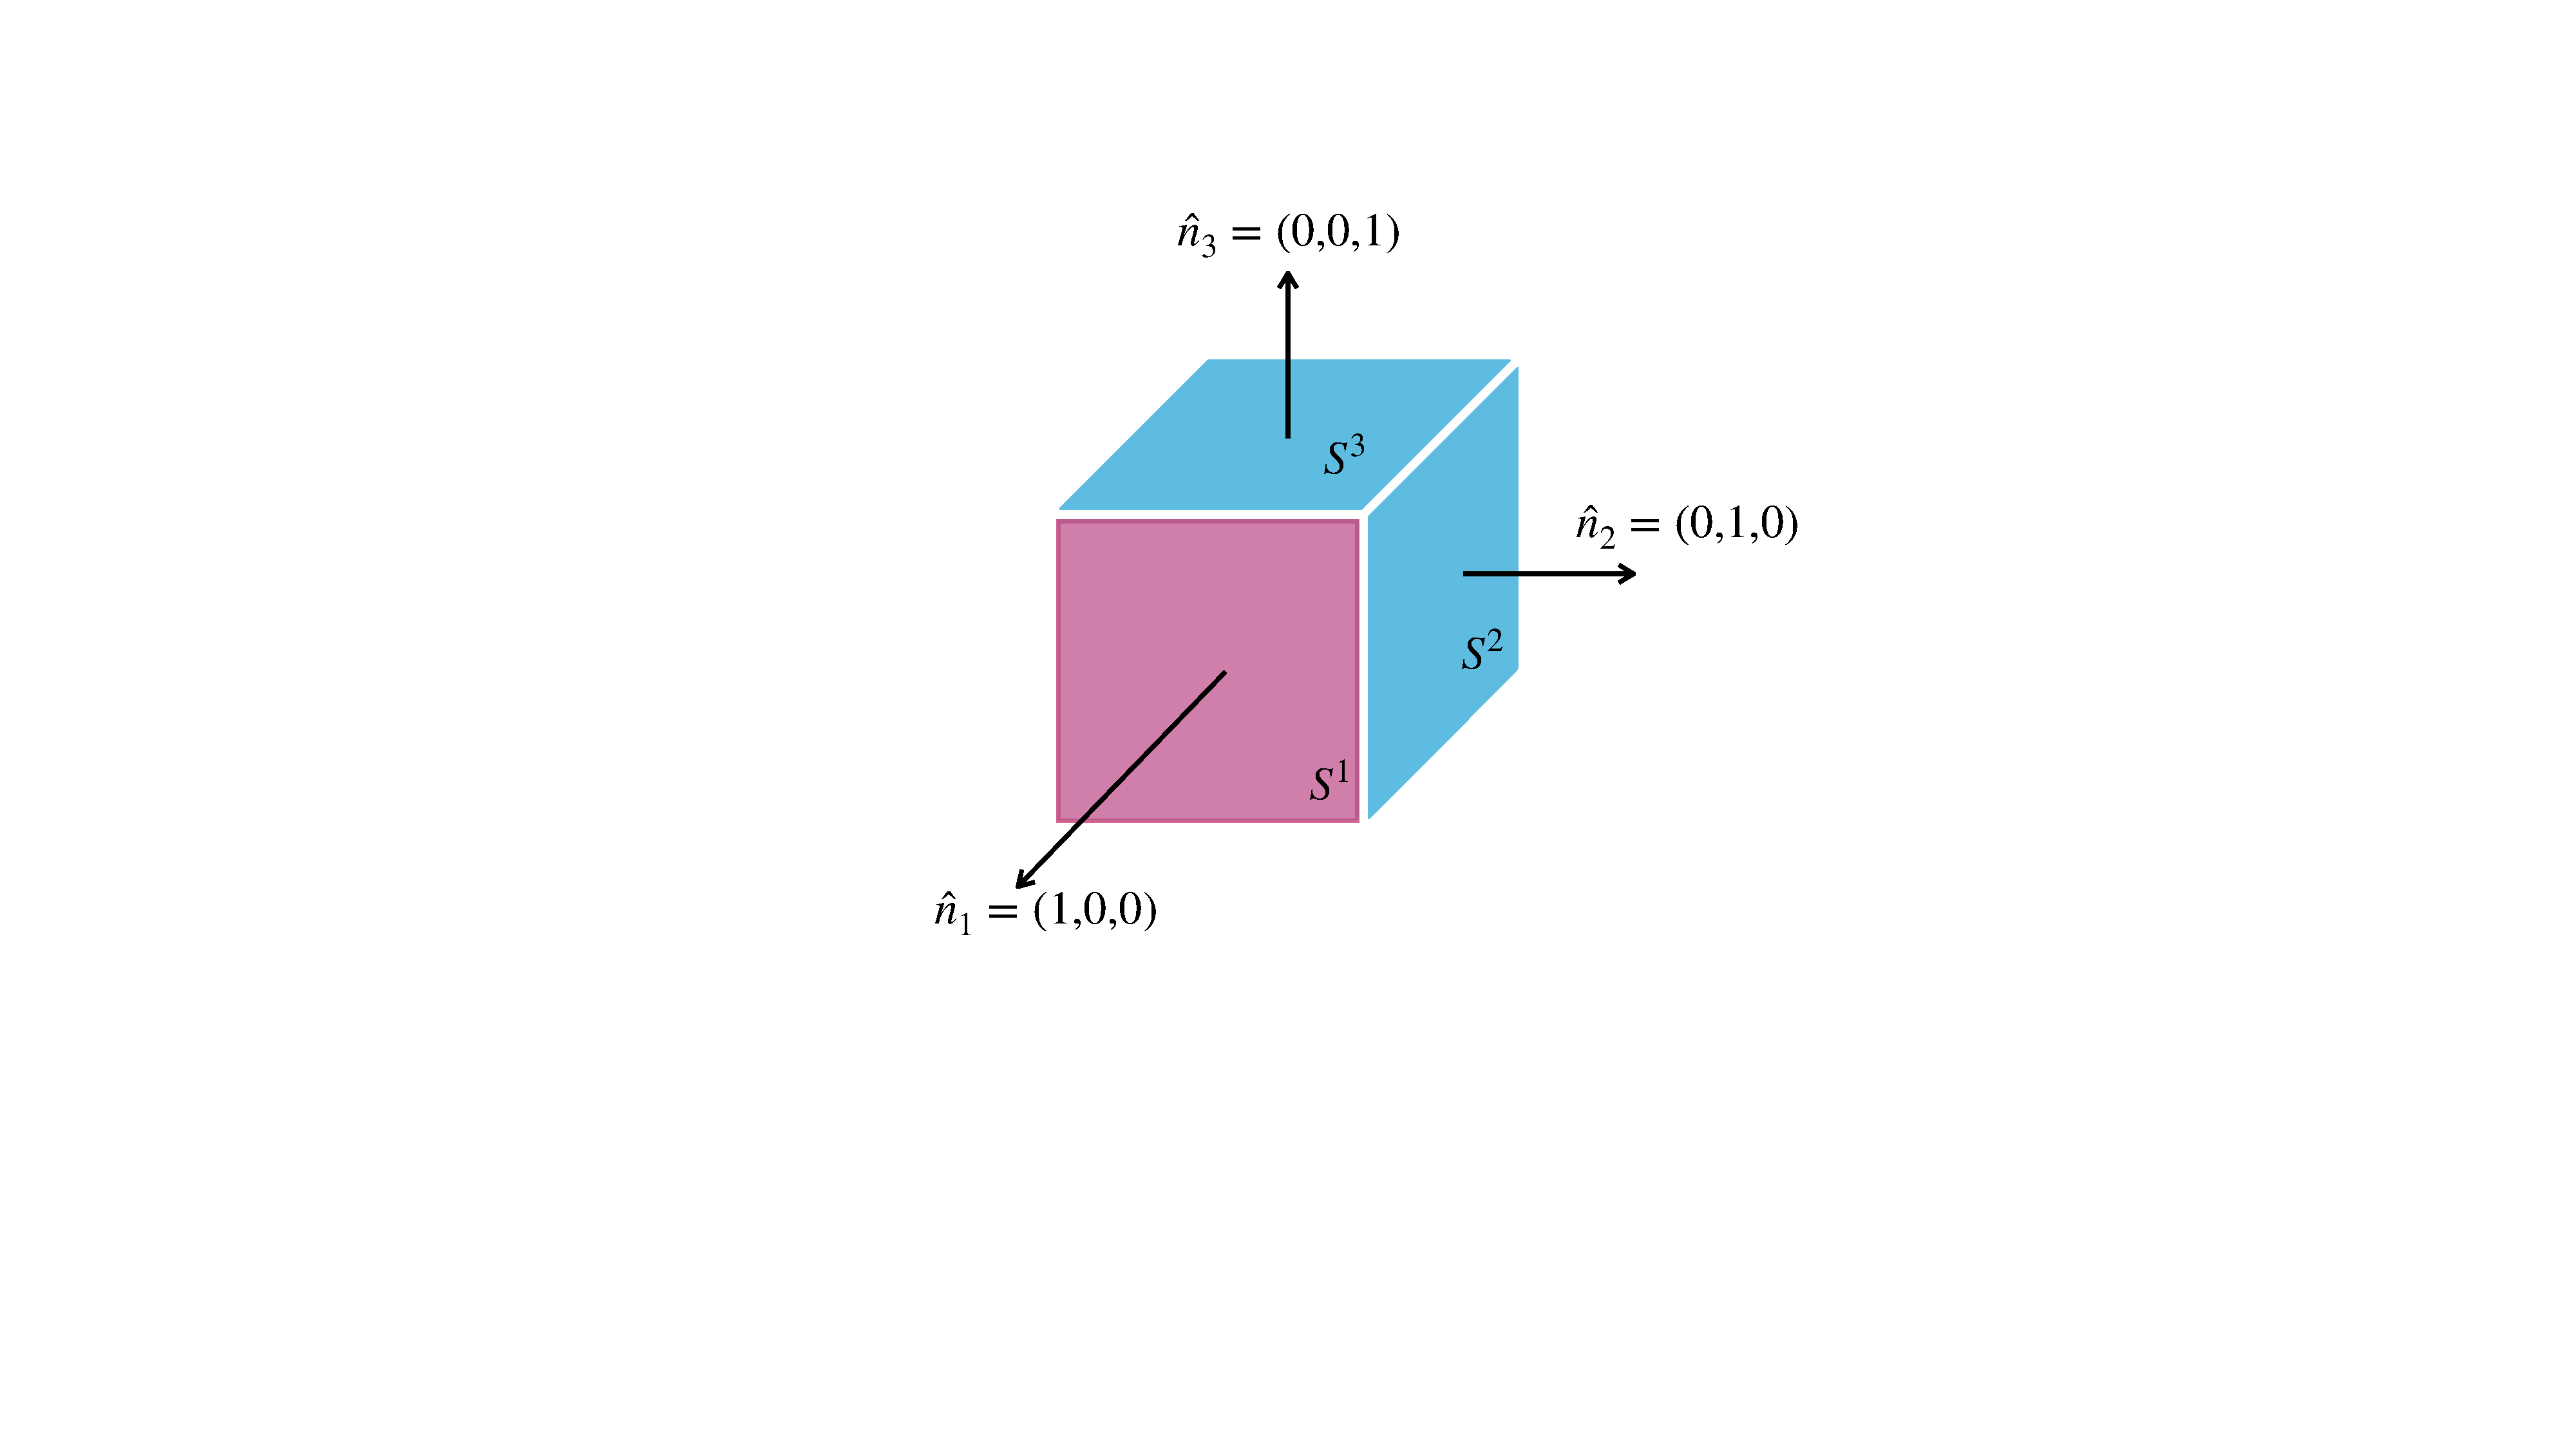
\includegraphics[scale=0.3]{./figures/fig_rho_bg_on_S1.pdf}
	\caption{Example cube to describe the buoyancy force computation. The pink area is the $S^1$ integral domain.}
	\label{fig_rho_bg_on_S1}
\end{center}
\end{figure}
Since the background density $\rho_{bg}$ is a function of $z$-axis only, we can intuitively see that the value (\ref{eq_buoyancy_S1_2}) and the one with the normal $\hat{n}_6 = -\hat{n}_1 = (-1,0,0)$ has the same magnitude but in the opposite direction, and thus, we have $\mathcal{L}_6 = -\mathcal{L}_1$. 
It implies the following.
\begin{equation}
	\sum_{i=1,2,5,6}
	 R_a^3 \int_{S^i} 
	 \mathcal{P}_{bg}(z) 
	 \bar{\bar{I \ }}  \cdot
	\hat{n}_i \ \textrm{d}S^i (\vec{x})
	 = 0
\label{eq_buoyancy_zero_oneCube}
\end{equation}
for the one cube case of discretized buoyancy equation (\ref{eq_buoyancy_discrete2}).
\par
The integrals on $S^3$ and $S^4$ are slightly different since the square faces are perpendicular to $z-$axis. On the face $S^3$, which has normal $\hat{n}_3 = (0,0,1)$, we get
\begin{equation}
	R_a^3
\rho_0\int_{-1}^{1} \int_{-1}^{1}
  	\left( 
  	 z - \frac{\gamma}{2}{z}^2 
 	\right)g  \bar{\bar{I \ }}  \cdot
 	\hat{n}_3 \ 
	\textrm{d}x  \textrm{d}y 
	= 4 R_a^3 \rho_0 \left( z_T - \frac{\gamma}{2} {z_T}^{2} \right) g \hat{n}_3,
	\label{eq_F_by_S3}
\end{equation} 
where $z_T$ is the constant $z-$level value on the face $S^3$. The integral value on the face $S^4$ would be the same as (\ref{eq_F_by_S3}), having $\hat{n}_4 = (0,0,-1)$ instead of $\hat{n}_3$. We then can have a more explicit expression for the discretized buoyancy equation (\ref{eq_buoyancy_discrete2}),
\begin{align}
	& \sum_{i=1}^{6} R_a^3
	 \int_{S^i}
	 \mathcal{P}_{bg}(z) 
	  g \bar{\bar{I \ }}  \cdot
	\hat{n}_i \ \textrm{d}S^i (\vec{x})
	\nonumber 
	\\
	& = 4 R_a^3 \rho_0 \left( z_T - \frac{\gamma}{2} {z_T}^{2}  \right) g \hat{n}_3
	+ 4R_a^3 \rho_0 \left( z_B - \frac{\gamma}{2} {z_B}^{2}  \right) g \hat{n}_4,
\label{eq_buoyancy_discrete_eval2}
\end{align}
where $z_B$ is the constant $z-$ value of the surface $S^4$ (bottom face). By substituting the normals $\hat{n}_3$ and $\hat{n}_4$, we can simplify the right-hand side of equation (\ref{eq_buoyancy_discrete_eval2}), knowing that $z_T - z_B = 2$, the equation (\ref{eq_buoyancy_discrete_eval2}) becomes 
\begin{equation}
	\sum_{i=1}^{6} R_a^3
	\int_{S^i} 
	\mathcal{P}_{bg}(z) 
	g \bar{\bar{I \ }}  \cdot
   \hat{n}_i \ \textrm{d}S^i (\vec{x})
= 8 R_a^3 \rho_0 \left( 1 - \gamma z_{c_n} \right) g, 
\label{eq_buoyancy_z_eval2}
\end{equation}
where we define the $z-$component of the center of $n-$th cube forming an aggregate, $z_{c_n}$ ($ n = 1, 2, \cdots, NC$).
We thus have shown that the only information we need to keep track of is the location of the center of each cube that forms an aggregate.
%
 \subsection{Linear system for velocity and stress on aggregates}
As mentioned in section~\ref{sec:force_balance}, we do not prescribe the settling velocity of an aggregate, and it becomes one of our unknowns.
We thus need to solve for 1) translational velocity ($\vec{U}_a$), 2) rotational velocity ($\vec{\Omega}$), and 3) stress vector ($\vec{f}_k$) on each square face $k$.
% To do so, we build a linear system using equations (\ref{eq_Fo}), (\ref{eq_Qo}). 
To do so, for any point $\vec{y}$ on the surface of the aggregate, we consider the surface velocity equations (\ref{eq_vel_all_onS_nonD}) with the solid body motion, (\ref{eq_solidbody}), 
 \begin{align}
	\vec{U}_a + \vec{\Omega} \times (\vec{y} - \vec{x}_{cm})
+ \frac{1}{8 \pi} \int_{S}  
		  \vec{f}(\vec{x}) 
		  \cdot \bar{\bar{G  }} (\vec{x},\vec{y}) 
		  \ \textrm{d}S(\vec{x})
		  \nonumber \\
=  -\frac{ \alpha C_{max}}{8\pi } \frac{\rho_0}{(\rho_s - \rho_0)(1-\phi)} 
\int_{V} C\left(\vec{x},  t \right) \hat{k} \cdot 
\bar{\bar{G}}(\vec{x}, \vec{y} ) 
\ \text{d}V(\vec{x}),
 \label{eq_slp_lin_eq}
 \end{align}
where the volume integral value on the right-hand side is known. 
To set up the linear system accordingly, We discretize the boundary integral as described in equation (\ref{eq_discretized}), choosing $\vec{f}_k$ for $\vec{q}_k$, and $ \bar{\bar{G}}$ for $\bar{\bar{J}}$, 
\begin{equation}
	\vec{I}(\vec{x}_{sq,i})  =   \sum_{k=1}^{N_f}  \vec{f}_k   \int_{S_{k}} \bar{\bar{G}}(\vec{x},\vec{x}_{sq,i}) \ \text{d}S(\vec{x}) 
	= \sum_{k=1}^{N_f} \vec{f}_k   \ \bar{\bar{\Pi}}_{i,k}
	\approx \int_{S}  
	\vec{f}(\vec{x}) 
	\cdot \bar{\bar{G  }} (\vec{x},\vec{x}_{sq,i}) 
	\ \textrm{d}S(\vec{x}),
\end{equation}
where $\vec{x}_{sq, i}$ is the center of each square on the surface for $i = 1, \  2, \cdots, \  N_f$.
With equations (\ref{eq_Fo}), (\ref{eq_Qo}), the exact linear system of the equations we implement is as follows.
 \begin{align}
	\tiny
		%---A------------------------------------------------------------
 	\left[
 	    \begin{array}{c;{2pt/2pt}c; {2pt/2pt}c}
 			\phantom{,} & \phantom{,}& \phantom{,}
 			\\
		   \begin{bmatrix}
 				\bar{\bar{\Pi}}_{1,1} & 
 				\bar{\bar{\Pi}}_{1,2} &
 				\cdots & \bar{\bar{\Pi}}_{1,N_f}
 				\\
 				\\
 				\bar{\bar{\Pi}}_{2,1} & 
 				\bar{\bar{\Pi}}_{2,2} &
 				\cdots & \bar{\bar{\Pi}}_{2,N_f}
 				\\ 
 				\vdots &  \vdots & \ddots & \vdots
 				\\
 				\\
 				\bar{\bar{\Pi}}_{N_f,1}&
 				\bar{\bar{\Pi}}_{N_f,2} &
 				 \cdots & \bar{\bar{\Pi}}_{N_f,N_f}
 		\end{bmatrix}
 			 & 
 			 \begin{bmatrix}
 				 \bar{\bar{I \ }}
 				 \\
 				 \vdots
 				 \\
 				 \\
 				  \bar{\bar{I \ }}
 			\end{bmatrix}
 			  & -
    			 \begin{bmatrix}
    				  [\vec{x}_{sq,1} - \vec{x}_{cm}]_{\times}
    				 \\
    				 \vdots
    				 \\
    				 \\
    				   [\vec{x}_{sq,N_f} - \vec{x}_{cm}]_{\times}
    			\end{bmatrix}
 			\\
 			\phantom{,} &\phantom{,} &\phantom{,}
 			\\
 			\hdashline[2pt/2pt]
 			\phantom{,} &\phantom{,} &\phantom{,}
 			\\
 			 4 \begin{bmatrix}
 				  \bar{\bar{I \ }}
 				 &
 				 \cdots
 				 &
 				  \bar{\bar{I \ }}
 			\end{bmatrix}
 			&  \bar{\bar{0}}  & \bar{\bar{0}}
 			\\
 			\phantom{,} &\phantom{,} &\phantom{,}
 			\\
 			 \hdashline[2pt/2pt]
 			 \phantom{,} &\phantom{,} &\phantom{,}
 			\\
 			 - 4 \begin{bmatrix}
 				[\vec{x}_{sq,1} - \vec{x}_{cm}]_{\times}
 				 &
 				 \cdots
 				 &
 				  [\vec{x}_{sq,N_f} - \vec{x}_{cm}]_{\times}
 			\end{bmatrix}
 			& \bar{\bar{0}}  &  \bar{\bar{0}}
  	 	\\
 			\phantom{,} & \phantom{,}& \phantom{,}
 	    \end{array}
 	\right]
 	%---x------------------------------------------------------------
 	\left[
 	\begin{array}{c}
 		\vec{f}_1
 		\\ \\
 		\vdots \\
 		\\
 		\vec{f}_{N_f}
 		 \\ \\  \hdashline[2pt/2pt]
 		\\
 		 \vec{U}_a
 	  	\\
 	 	\\
 	 	\hdashline[2pt/2pt]
 	 	\\
 	 	\vec{\Omega}
 	\end{array}
 	\right]
 		%---b------------------------------------------------------------
 	=
 	\left[
 	\begin{array}{c}
 		{\vec{\mathcal{F}}}^1  \\ \\
 		\vdots \\
 		\\
 		{\vec{\mathcal{F}}}^{N_f} \\ \\  \hdashline[2pt/2pt]
 		\\
 		 \vec{F}_o
 	  	\\
 	 	\\
 	 	\hdashline[2pt/2pt]
 	 	\\
 	 	\vec{Q}_o
 	\end{array}
 	\right].
 \label{eq_slp_linear_system}
 \end{align}
 Since we consider three-dimensional space, the size of the identity matrix $\bar{\bar{I}}$ is $(3 \times 3)$. The matrix $[\vec{y}]_{\times}$ represents the cross product operator defined by,
 \begin{equation}
 	[\vec{y}]_{\times} = \begin{bmatrix}
 	0 & -y_3  & y_2 \\ 
 	 y_3 & 0  & -y_1\\ 
 	- y_2 & y_1  & 0
 	\end{bmatrix},
 	\label{eq_cross_2}
 \end{equation}
 where $\vec{y} = (y_1, y_2, y_3).$
We use this operator for the rotation term, 
 \[
  [\vec{x} - \vec{x}_{cm}]_{\times}  \vec{\Omega}
   = (\vec{x} - \vec{x}_{cm}) \times \vec{\Omega}
  = - \vec{\Omega} \times  (\vec{x} - \vec{x}_{cm}),
  \]
in the total torque equation.
In addition, the top part of the right-hand side of the equation (\ref{eq_slp_lin_eq}) is the discretization of the volume integral,
\begin{equation}
	{\vec{\mathcal{F}}} (\vec{x}_{sq,i}) = 
	-\frac{ \alpha C_{max}}{8\pi } \frac{\rho_0}{(\rho_s - \rho_0)(1-\phi)} 
   \sum_{j= 1}^{Ns}  C \left(\vec{x}_{sq,i},  t \right) \hat{k} \cdot
   \bar{\bar{G \ }}(\vec{x}_{sq, i}, \vec{x}_{j} ),
\label{eq_volume_rhs}
\end{equation}
   where $N_s$ is the total number of grid or source points in the fluid domain. We discuss more details of the volume integral computation in the next section. 
%   ~\ref{section_volume_int}.
  One can find factor 4 multiplied by the second and third blocks on the right-hand side of the system (\ref{eq_slp_linear_system}). 
 Since we set the side length of a cube as 2, factor 4 represents the area of a square face that is the integral domain of the total force and torque equations. 
 \par
 Once we solve the linear system and obtain the unknowns, we use the equation (\ref{eq_vel_all_onS_nonD}) to calculate the velocity field at all points in the fluid domain. We want to point out that the fluid velocity computation, especially including the volume integral (\ref{eq_volume_rhs}), is a very numerically expensive calculation. To accelerate it, we apply the fast multipole method (FMM) to our simulations. In the following section, we explain how we use the FMM. 
 %
 %
 %----FMM--------------------------------------------------------------------------
\subsection{Fast Multipole Method (FMM)}
\label{subsec:FMM}
Knowing that we simulate our problem in a three-dimensional fluid domain, it is necessary to implement an efficient and fast method for each part of the codes while we keep the stability and desired accuracy. 
The FMM is a numerical scheme for rapid computation of $N$-body problems governed by a Green's function using a multipole expansion. It was first introduced by Greengard and Rokhlin~\cite{greengard_fast_1987}. Since then, the researchers at Flatiron Institute - Simons Foundation,  including the original authors of the FMM, have developed the methods and shared the source code.~\cite{cheng_fast_1999,greengard_new_1997,greengard_new_2002} We choose to use their library, called \href{https://github.com/flatironinstitute/FMM3D}{{\color{blue}FMM3D}}. It provides the code of the $N-$body interactions governed by Laplace and Helmholtz equations in three-dimension.
For our problem, we can modify the Laplace kernel, as shown in~\cite{tornberg_fast_2008}, to compute the integrals of Stokeslet (\ref{eq_stokeslet}).
The definition of Laplace FMM in the FMM3D library is the following:
\begin{definition} (\textit{Laplace FMM})
	\label{eq_def_FMM}
	Let $c^n \in \mathbb{R}$ denote a collection of charge strengths and $\vec{v}^n \in \mathbb{R}^3$ denote a collection of dipole strengths for $n = 1,2, \cdots, N$.
	The Laplace FMM computes the potential $u(\vec{y}^m) \in \mathbb{R}^3$ given by
\begin{equation}
	u(\vec{y}^m) = \sum_{n = 1}^{N} 
		\Biggl[
		\frac{c^n}{\|\vec{x}^n - \vec{y}^m \|}
			- \vec{v}^n \cdot \nabla_{\vec{y}} 
			 \frac{1}{\|\vec{x}^n - \vec{y}^m \|}
		\Biggr],
\label{eq_fmm3d_package}
\end{equation}
	at the \textit{source} ($\vec{x}^n$) and \textit{target} locations ($\vec{y}^m$). 
	% Here, the denominator $\|x_i^n - y_j^m \| = \|\vec{x}^n - \vec{y}^m \|$.
	When $\vec{y}^m = \vec{x}^n$, the term corresponding to $\vec{x}^n$
	is dropped from the sum.
\end{definition}
\noindent
Note that we use the letters $m$ and $n$ to index the targets and sources, respectively. For our problem, the points where we want to obtain velocity would be the targets; all points in an integral domain are sources.
In addition to the target and source points, we can input the constant $c^n$ and vector $\vec{v}^{n}$. One needs to be careful about these terms; both values could depend on the sources but are independent of the targets. 
\subsubsection{Volume integral of the Stokeslet}
We first investigate how to incorporate the volume integral (\ref{eq_volume_rhs}) (without the prefactor) in the form of (\ref{eq_fmm3d_package}). For a fixed $j$, we can rewrite the equation using the index notation ($i, j = 1,2,3$), 
\begin{equation}
	\tilde{V}(y_j^m)
	\equiv
	 d\sum_{n = 1}^{Ns} \sum_{i = 1}^{3}
	 C(x^n_i,  t)\hat{k} G_{ij}(x_i^n,y_j^m),
	\label{eq_Vn}
\end{equation}
where $\vec{y}^m = (y_1^m, \ y_2^m, \ y_3^m)$ is the target point, $\vec{x}^n = (x_1^n, \ x_2^n, \ x_3^n)$ are the source or grid points in the fluid domain $V$, and $d$ is constant from a quadrature method.
Note that we can use the FMM3D only for points $\vec{y}^m \neq \vec{x}^n \in V$. 
At a singularity, i.e.,  $\vec{y}^m = \vec{x}^n $, we use MATLAB built-in function, \verb+integral3+, to integrate numerically by defining a small cube $V_p$ around the singularity point,
\begin{equation}
	\mathbb{V}_p(\vec{y}) = 
	 \int_{{V}_p}
		C (\vec{x},t ) \hat{k} \cdot 
		\bar{\bar{G \ }} (\vec{x}, \vec{y} ) 
		\ \text{d}V(\vec{x}).
		\label{eq_vol_int_singular}
	\end{equation}
We then compute $\tilde{V}$ as in equation (\ref{eq_Vn}).
The Stokeslet can be expressed in terms of the Laplace kernel, $\Phi(\vec{x},\vec{y}) = 1/{\| \vec{x} - \vec{y} \|}$ as,
\begin{equation}
	G_{ij}(\vec{x}^n, \vec{y}^m)
	 =  \delta_{ij} \Phi \left(  x_i^n - y_j^m\right)
	 - \left( x_i^n - y_j^m \right)
	 \frac{\partial}{\partial  x_j}
	\Phi \left(  x_i^n - y_j^m\right)
	\label{eq_Gij}
\end{equation}
% Then the inner summation of equation (\ref{eq_Vn}) becomes
% \begin{align*}
%  \sum_{i = 1}^{3}
%  C(x^n_i,  t)\hat{k} G_{ij}(x_i^n,\vec{y}^m)
%  	=  \sum_{i = 1}^{3} C(x^n_i,  t)\hat{k}
% 	\left(
% 	\frac{\delta_{ij}}{\|x_i^n - y_j^m \|}
% 	- \left( x_i^n - y_i^m \right)
% 	 \frac{\partial}{\partial x_j}
% 	\frac{1}{\|x_i^n - y_j^m \|}
% 	\right)
% \end{align*}
By substituting the Stokeslet (\ref{eq_Gij}) into the discretized volume integral (\ref{eq_Vn}), we then get
\begin{equation}
	\tilde{V}_j (\vec{y}^m)=
	\sum_{n=1}^{Ns}
	d
   \sum_{i = 1}^{3} C(x^n_i,  t)\hat{k}
  	\left(
  	\frac{\delta_{ij}}{\| \vec{x}^n - \vec{y}^m \|}
  	- \left( x_i^n - y_j^m \right)
  	 \frac{\partial}{\partial x_j}
  	\frac{1}{\| \vec{x}^n - \vec{y}^m \|}
  	\right)
 \label{eq_frm_lplc_stokes}
\end{equation}
Knowing that the vector $\hat{k} = (0, \ 0, \ 1)$, only the terms where $i = 3$ survive. We thus reach the simplified sum (\ref{eq_frm_lplc_stokes}),

\begin{align}
	\tilde{V}_j (\vec{y}^m) 
	& = \sum_{\substack{n=1 \\ n \neq m}}^{Ns} 
		d \ {C}(x_3^n, t)
		\left(
			\frac{ \delta_{3j} }{\|\vec{x}^n - \vec{y}^m \|}
			- 
			 x_3^n  
			\frac{\partial}{\partial x_j}
				\frac{1}{\|\vec{x}^n - \vec{y}^m \|}
				\right)
			\label{eq_vol_target} \\
			& +
			   y_j^m  
			\sum_{\substack{n=1 \\ n \neq m}}^{Ns} 
			d \ {C}(x_3^n, t)
			\frac{\partial}{\partial x_j}
				\frac{1}{\|x_3^n - y_j^m \|} + \mathbb{V}_p.
\label{eq_vol_source}
\end{align}
We split the gradient term into two parts since the nature of $x_3^n$ and $y_j^m$ differs. We see that $x_3^n$ relates to the source point as the FMM3D package does. However, $y_j^m$ is the target. 
% We thus need to use the library twice to compute $\tilde{V}_j (\vec{y}^m) $.
The main advantage of this method is that we need to call this Laplace FMM code only once for multiple targets and $N$ number of source points. 
Note that the FMM3D package returns a scalar value. Meanwhile, our summation has a vector form. We thus need to run this package three times at least for each part, (\ref{eq_vol_target}) and (\ref{eq_vol_source}). For more details, we break down the equations to determine what are $c^n$ and $\vec{v}^n$ would be.
\par
First, we consider the first term in summation (\ref{eq_vol_target}),
\begin{align}
	\sum_{\substack{n=1 \\ n \neq m}}^{Ns} 
		d \ {C}(x_3^n, t)
			\frac{ \delta_{3j} }{\|x_3^n - y_j^m \|}
	 & = \left(0,\ 0, d 	\sum_{\substack{n=1 \\ n \neq m}}^{Ns}  \frac{ {C}(x_3^n, t)}{ \|x_i^n - y_j^m \|} \right)
\label{eq_vol_part1}
\end{align}
Since ${C}(x_3^n, t)\in \mathbb{R}$ for each $n$ and a fixed time $t$, we simply choose  $c^n =  {C}(x_3^n, t)$. 
The second term in the sum (\ref{eq_vol_target}) can be computed by letting $\vec{v}^n$ in equation (\ref{eq_fmm3d_package}) as a product of a standard basis vector, $\hat{e}_j$, and the constant $x_3^n  \ {C}(x_3^n, t) $, that is
\begin{align}
	\sum_{\substack{n=1 \\ n \neq m}}^{Ns} 
		d \ {C}(x_3^n, t)
		\left(
			 x_3^n  
			\frac{\partial}{\partial x_j}
				\frac{1}{\|\vec{x}^n - \vec{y}^m\|}
				\right) = 
		d \sum_{\substack{n=1 \\ n \neq m}}^{Ns} 
			x_3^n  \ {C}(x_3^n, t) 
			      \
			\nabla_{\vec{y}} 
				\frac{1}{\|\vec{x}^n - \vec{y}^m \|}.
\label{eq_vol_part2}
\end{align}
We simply repeat the FMM3D for each component. 
\par
As we mentioned, the second summation (\ref{eq_vol_source}) is slightly different since the target point is multiplied by the gradient term that can be only related to the sources. One of the critical rules in the FMM is separating the target and source terms to compute integrals rapidly. Thus, the computation of this sum requires another three uses of the FMM package and a dot product with the target point vector.
We compute the sum in the same manner as (\ref{eq_vol_part2})
\begin{equation}
	y_j^m  
	\sum_{\substack{n=1 \\ n \neq m}}^{Ns} 
	d \ {C}(x_3^n, t)
	\frac{\partial}{\partial x_j}
	\frac{1}{\| \vec{x}^n - \vec{y}^m \|} 
	= d y_j^m  
	\sum_{\substack{n=1 \\ n \neq m}}^{Ns}  
	{C}(x_3^n, t) \
	\nabla_{\vec{y}} 
	\frac{1}{\| \vec{x}^n - \vec{y}^m\|}
\end{equation}
as we have shown in the previous summation term with the gradient. 
%---------Homogeneous velocity computation---------------------------------------
\subsubsection{Surface integral of the Stokeslet}
To obtain the fluid velocity, we use equation (\ref{eq_vel_all_onS_nonD}) for all $\vec{y} \in V$. In this computation, the evaluation of
\begin{equation}
	u_H(\vec{y})  
	= \int_S \vec{f}(\vec{x}) \cdot \bar{\bar{G \ }}( \vec{x}, \vec{y}) \ \text{d} S(\vec{x}),
	\label{eq_uH}
\end{equation}
is quite heavy computationally, as is that of the volume integral. 
We measured CPU time while varying the total number of fluid grid points. 
In Figure~\ref{fig_time_fmm_sum}, each line represents CPU time to compute, in seconds: 1) volume integral on the aggregate surface $S$, 2) volume integral in the fluid domain $V$, 3) solve for the linear system, 4) solve the advection-diffusion equation to update the perturbation, 5) velocity evaluation in the fluid domain, and 6) sum of all above (1 - 5).
\begin{figure}[ht]
	\begin{center}
		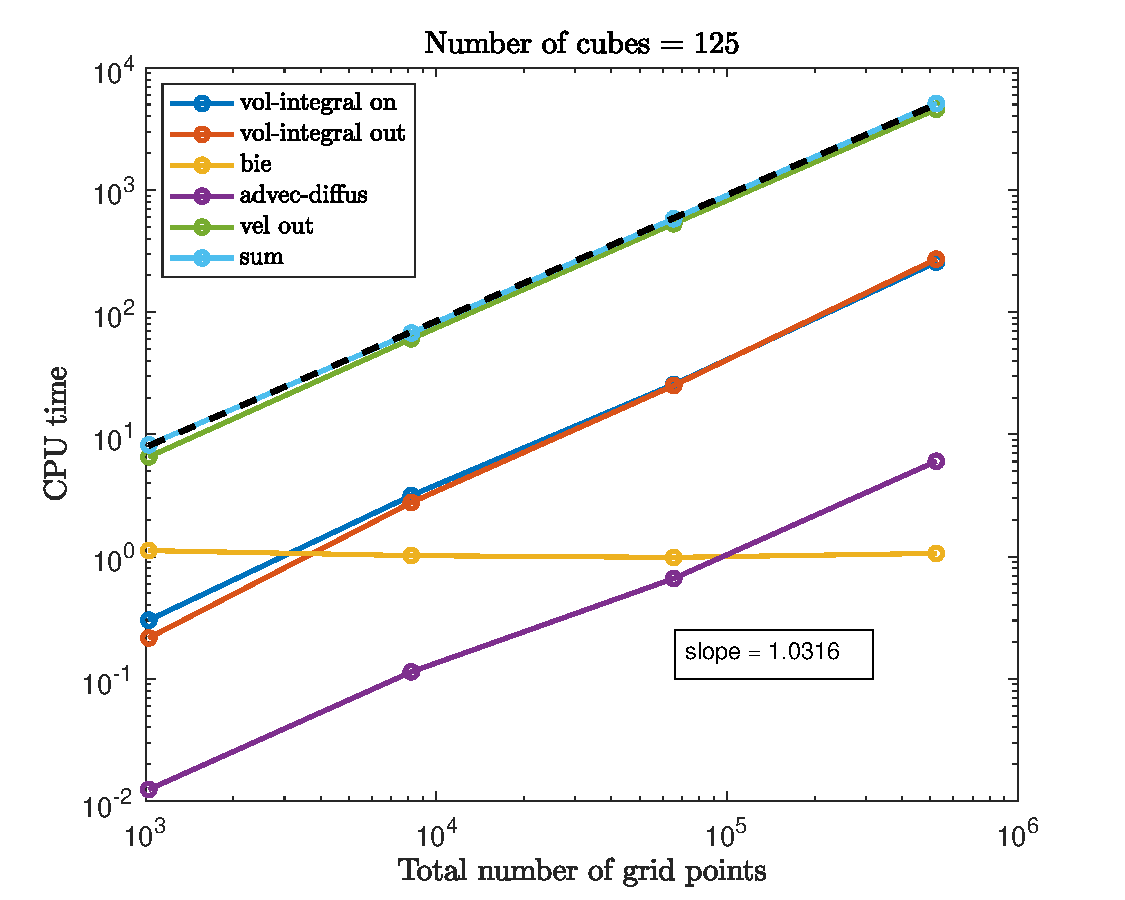
\includegraphics[scale=0.45]{./figures/fig_time_varNx5}
		% 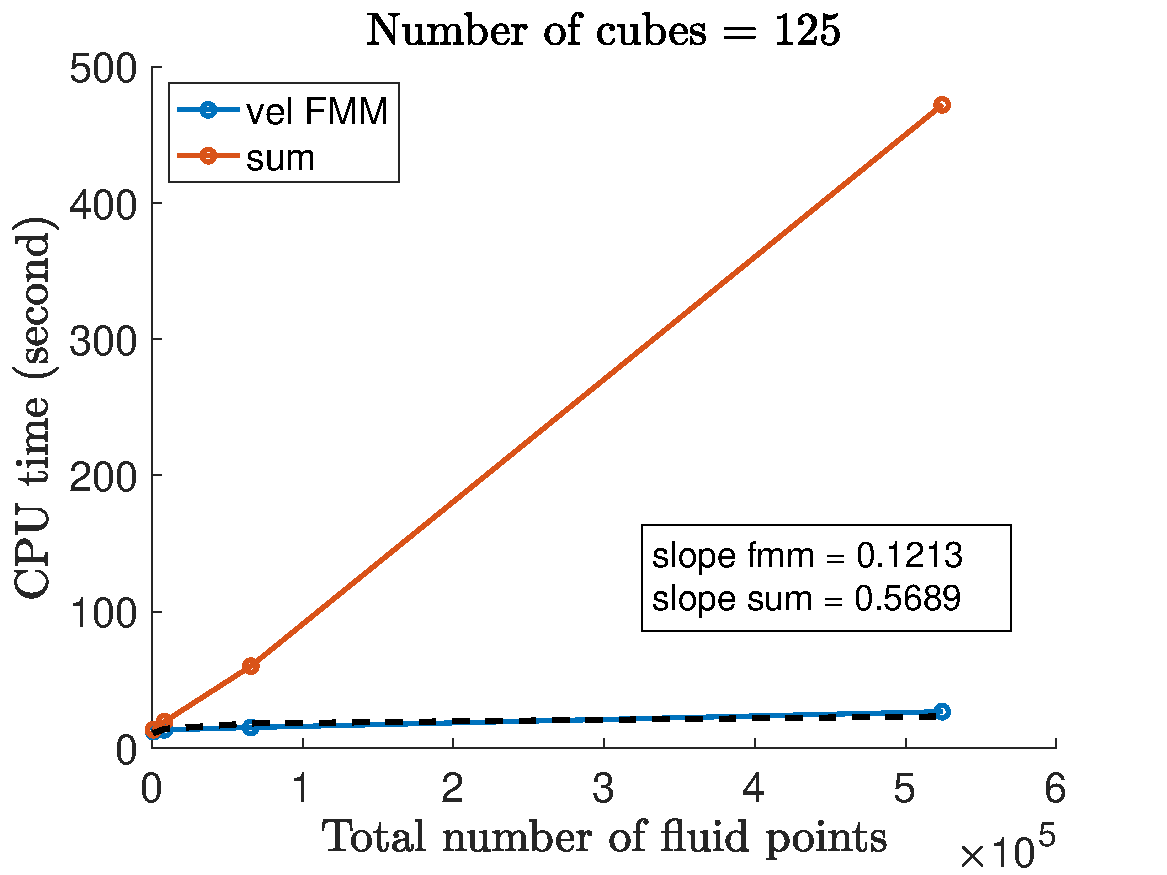
\includegraphics[scale=0.45]{./figures/fig_time_fmm_sum}
	\caption{CPU time in second with an aggregate of 125 cubes for ten time-steps.}
	\label{fig_time_fmm_sum}
\end{center}
\end{figure}
The main takeaway in this plot is that the velocity computation for all fluid points is dominant. 
We thus decided to use the FMM for this surface integral by approximating as follows:
Here, the points $\vec{x}$ are the sources, and $\vec{y}$ are the targets. 
For the velocity inside and on the aggregate boundary, we use the rigid boundary velocity $u(\vec{x}) = \vec{U}_a + \vec{\Omega} \times \left(\vec{x} - \vec{x}_{cm} \right)$. This implies that we only use targets located outside the aggregate, and we do not expect any singularity in this computation ($\vec{x} \neq \vec{y}$). However, we may have close evaluation problems. We will discuss the size of errors in the next section. 
\par
We handle the integration of the Stokeslet in a manner similar to what was done for the volume integral. 
Using the Laplace kernel, we can re-write the surface integral (\ref{eq_uH}) as
\begin{equation}
	u_H(\vec{y}) =
	\int_S 
	\vec{f}(\vec{x}) \cdot
  	\left(
  	\frac{\bar{\bar{I \ }}}{\|\vec{x} - \vec{y}\|}
  	- \left( \vec{x} - \vec{y} \right)
  	 \nabla_{\vec{y}}
  	\frac{1}{\|\vec{x} - \vec{y}\|}
  	\right)
	  \ \text{d} S(\vec{x}).
 \label{eq_surf_laplace}
\end{equation}
We first discretize the entire aggregate surface into $N_f$ square faces located at $[cx_j^n-1, cx^n_j+1]$, where $(cx^n_1, cx^n_2)$ is the center of $n-$th square face. The discretized version of the velocity equation (\ref{eq_surf_laplace}) is denoted by $H(\vec{y})$,
\begin{align}
	H(\vec{y}^m) & = u_H(\vec{y}) - E_f
	 = \sum_{n = 1}^{N_f} H^n(\vec{y}^m) 
	\nonumber \\
	& = \sum_{n = 1}^{N_f} 
	\vec{f}(\vec{x}^n) \cdot
	\int_{cx^n_2-1}^{cx^n_2+1} \int_{cx_1^n-1}^{cx_1^n+1}
  	\left(
  	\frac{\bar{\bar{I \ }}}{\|\vec{x}^n - \vec{y}^m\|}
  	- \left( \vec{x}^n - \vec{y}^m \right)
  	 \nabla_{\vec{y}^m}
  	\frac{1}{\|\vec{x}^n - \vec{y}^m\|}
  	\right)
	  \text{d} x_1  \text{d} x_2
	  ,
 \label{eq_surf_fmm_N_f}
\end{align}
where the error coming from this approximation is denoted as $E_f$. A more detailed analysis regarding $E_f$ can be found in section~\ref{sec:bie_validataion}.
 Note that the stress $\vec{f}(\vec{x}^n)$ is assumed to be constant over each square face.  One can find that we have a significant error in the cube's corners. We want to ensure that we do not introduce larger errors as we make further approximations. 

\par
Next, we need to approximate the surface integral in equation (\ref{eq_surf_fmm_N_f}) using a Riemann sum,
\begin{align}
	\tilde{H}(\vec{y}^m) 
	& = H^n(\vec{y}^m) - E_{G} 
	\nonumber \\ 
	& =
	\sum_{n = 1}^{N_f} 
	\vec{f}(\vec{x}^n) \cdot
	\sum_{s=1}^{Ns^2} d^2 
  	\left(
  	\frac{\bar{\bar{I \ }}}{\|\vec{x}_s^n - \vec{y}_s^m\|}
  	- \left( \vec{x}_s^n - \vec{y}^m \right)
  	 \nabla_{\vec{x}_s^n}
  	\frac{1}{\|\vec{x}_s^n - \vec{y}^m\|}
  	\right)
	  - E_{G},
 \label{eq_surf_fmm_N_f_n}
\end{align}
where $E_G$ is the error coming from the quadrature method. 
We use $N_s^2$ sub-squares with sizes of $d = 2/N_s$ and take the center of each sub-squares as the integration point. 
We take the same number of points, $N_s$, evenly distributed in one direction. 
In the following schematics, Figure~\ref{fig_face_grid}, the red cross represents the center of the $n-$th square face, $(cx^n_1, cx^n_2)$.
\begin{figure}[h]
	\begin{center}
		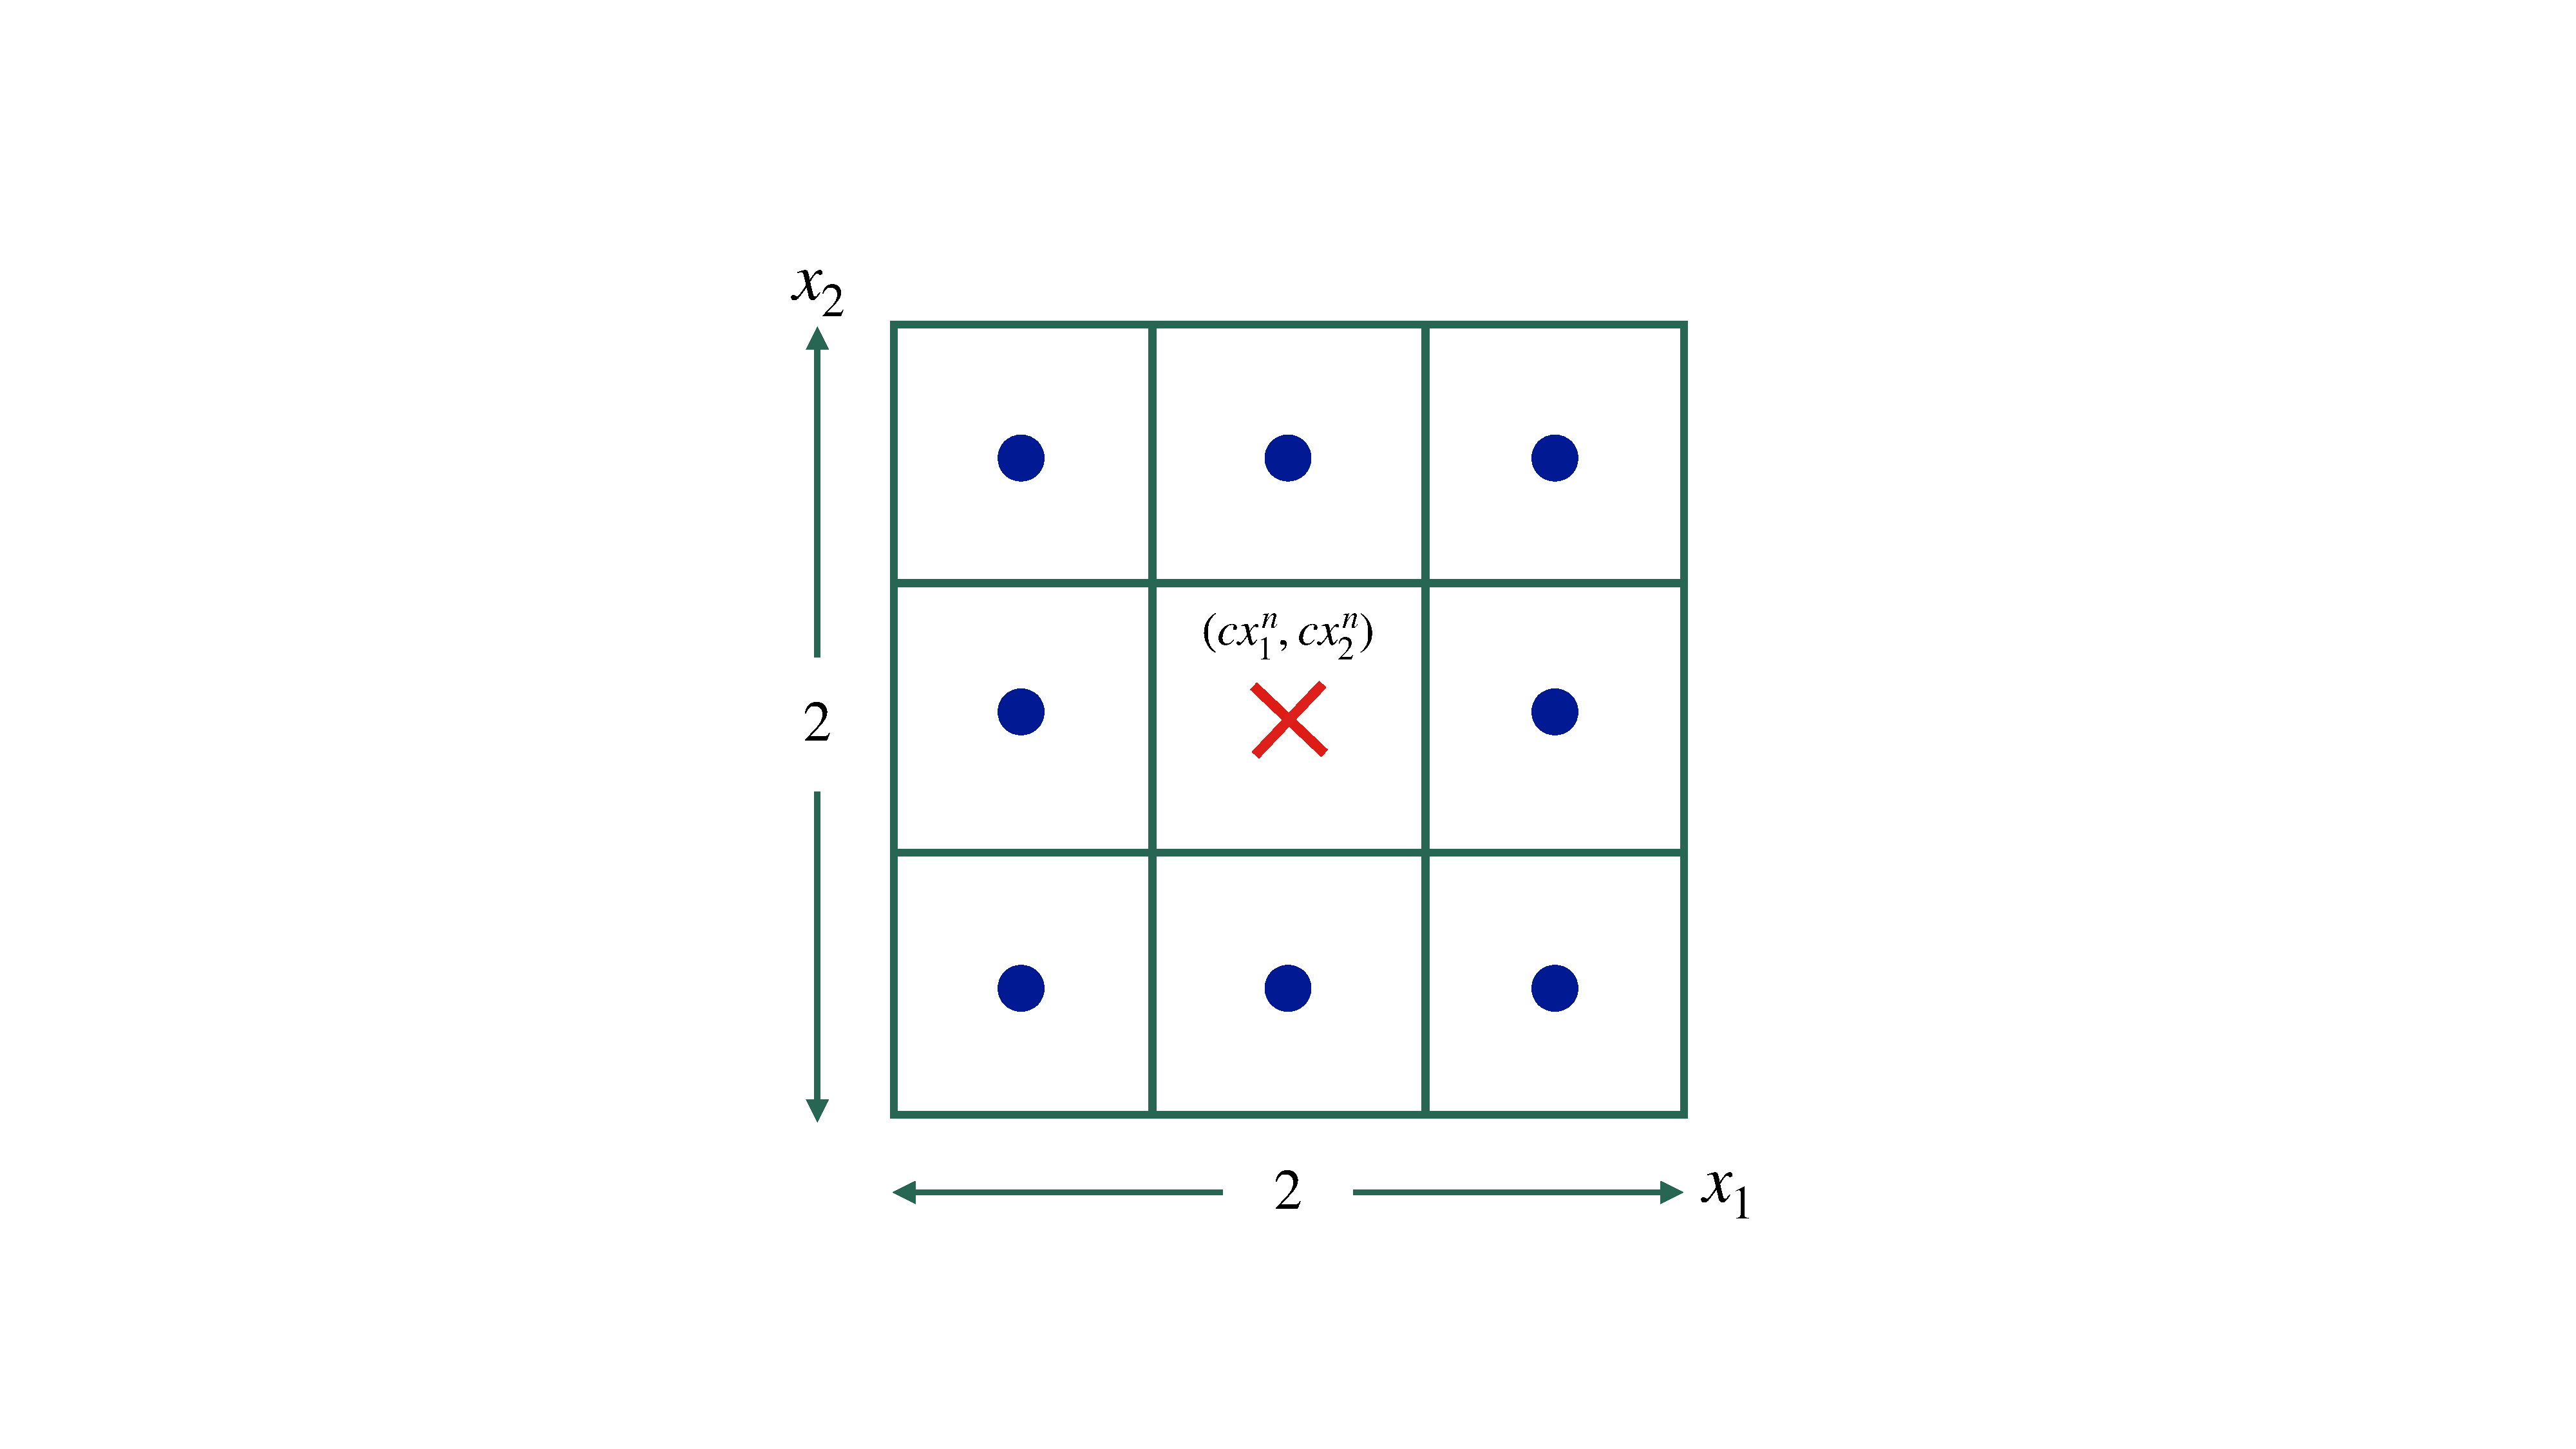
\includegraphics[scale=0.17]{./figures/fig_face_grid}
	\caption{Schematic of points we use to approximate the integral of the single-layer potential kernel over one square face.}
	\label{fig_face_grid}
\end{center}
\end{figure}
The blue dots and the red cross are the integration points.
We do not include any boundary values on one square face for simplicity.
\par
As mentioned, we hope to have a reasonable size of the integration error, i.e., $E_G \ll E_f$.
To measure $E_f$, we consider the settling of one cube shape aggregate.
We then observe the relative error of the vertical velocity on one square face, considering the translational velocity, $\vec{U}_a$, as the exact solution.
\begin{figure}[h]
	\begin{center}
		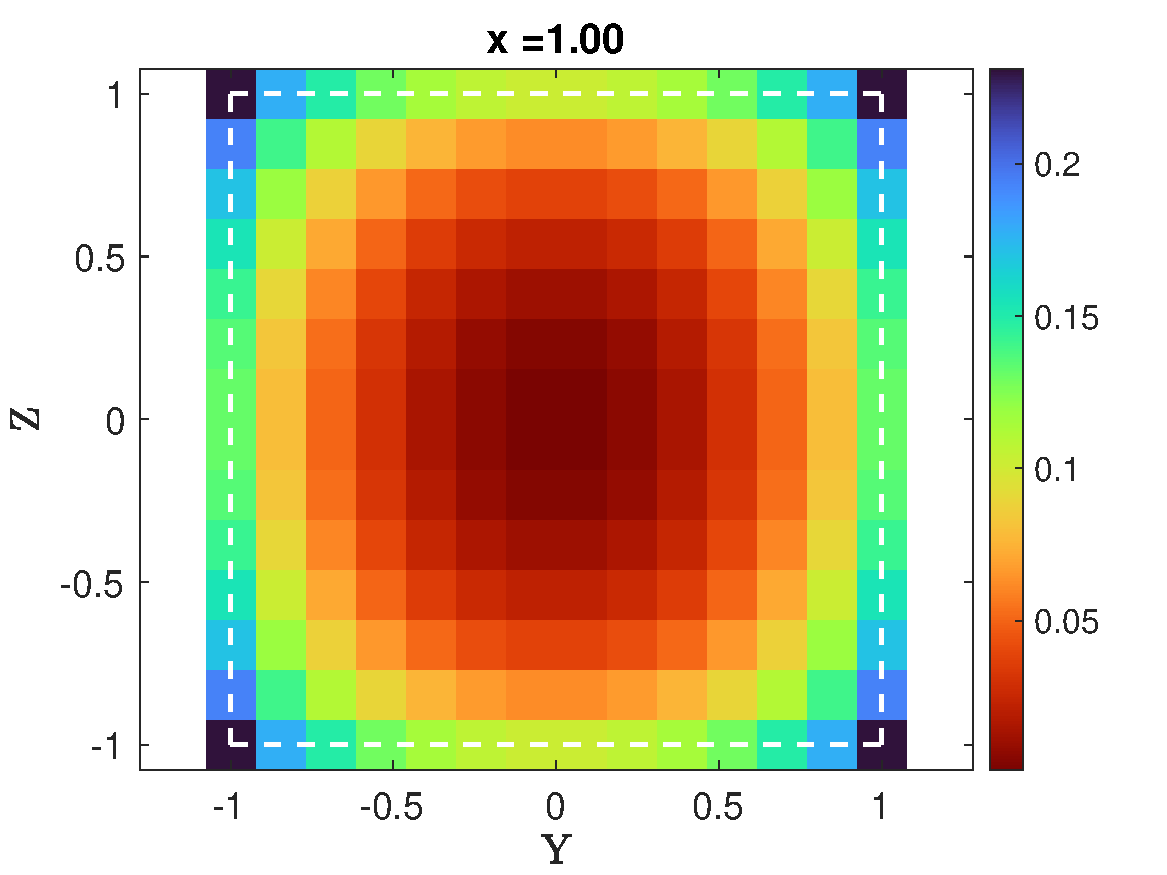
\includegraphics[scale=0.3]{./figures/fig_corner_err}
	\caption{Sample case of the relative velocity error on one face, $E_f$.}
	\label{fig_corner_err}
\end{center}
\end{figure}
In Figure~\ref{fig_corner_err}, we see the square face at $x = 1$, where the white dashed line shows the location of the square face, and the color indicates the relative error. It implies that the maximum of 23.12$\%$ error occurs at the cube's corner, as we expected. We thus would like to regulate the quadrature error, $E_G$, by adjusting the total number of integration points, $Ns^2$.
\par
Two parameters affect the efficiency and accuracy of the FMM computations: 1) the number of quadrature points and 2) the tolerance $\varepsilon$ in the FMM3D library, which determines the number of terms in the series expansion.
In Figure~\ref{fig_Ef_EG_compare}, we vary the number of integration points to choose an optimal value. 
\begin{figure}[ht]
	\begin{center}
		% 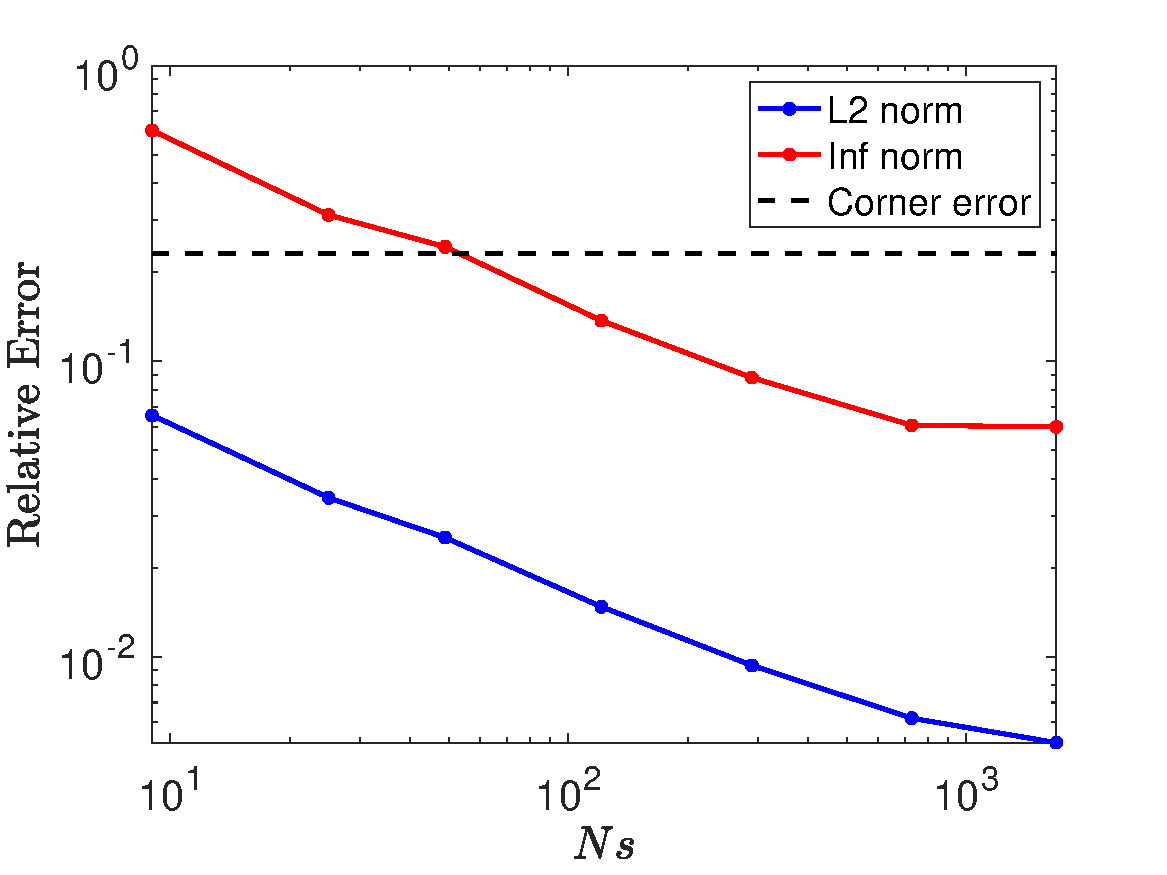
\includegraphics[scale=0.33]{./figures/fig_Ef_EG_compare}
		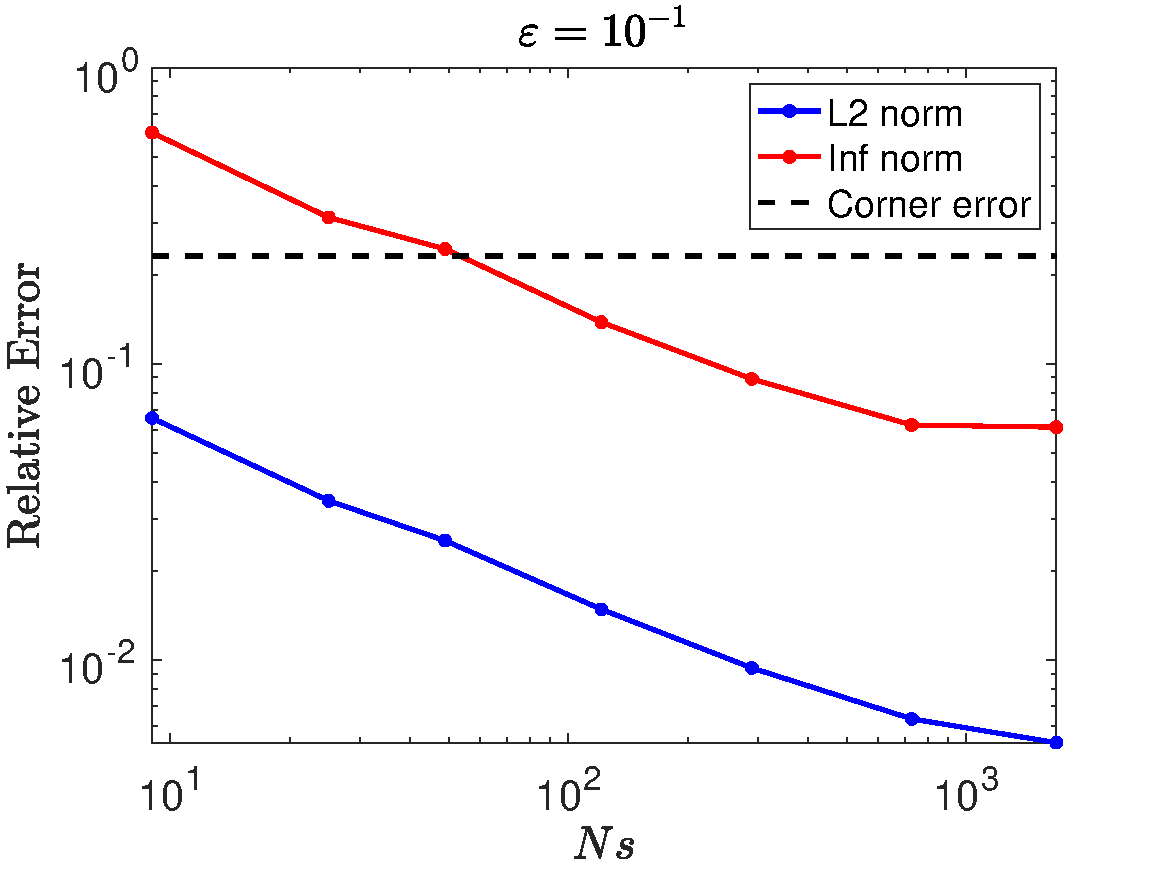
\includegraphics[scale=0.4]{./figures/fig_Ef_Eg_ep-1}
	\caption{Relative error between $U^*$ and $U^{*+}$, varying the number of integration points: $Ns = [3, 5, 7, 11, 17, 27,41]^2$ and $\varepsilon = 10^{-1}$.}
	\label{fig_Ef_EG_compare}
\end{center}
\end{figure}
We test a single-time simulation in the domain,  $[-5, 5] \times [-5, 5] \times [-10, 10]$,  with one cube aggregate model. To confirm the responses of $\varepsilon$ values, we simulate the same one with two tolerance values, $\varepsilon = 10^{-1}, \ 10^{-6}$.
From this analysis, we are convinced that $Ns = 9^2$ quadrature points are enough to satisfy the error size we can tolerate. It produces quite similar results for the $\varepsilon = 10^{-6}$ case. We did not notice any difference in accuracy. We may observe this because the corner error, $E_f$, dominates our approximation and is already larger than $10 \%$. 

After implementing the FMM3D library into our program, we timed one more time to compare the fluid velocity computation shown as the green (or dashed line) in Figure~\ref{fig_time_fmm_sum}. The efficiency of the computation increases about ten times when the number of fluid grid points is about 500,000, which is in the range of what we will use to compute the fully stratified simulations.
\begin{figure}[ht]
	\begin{center}
		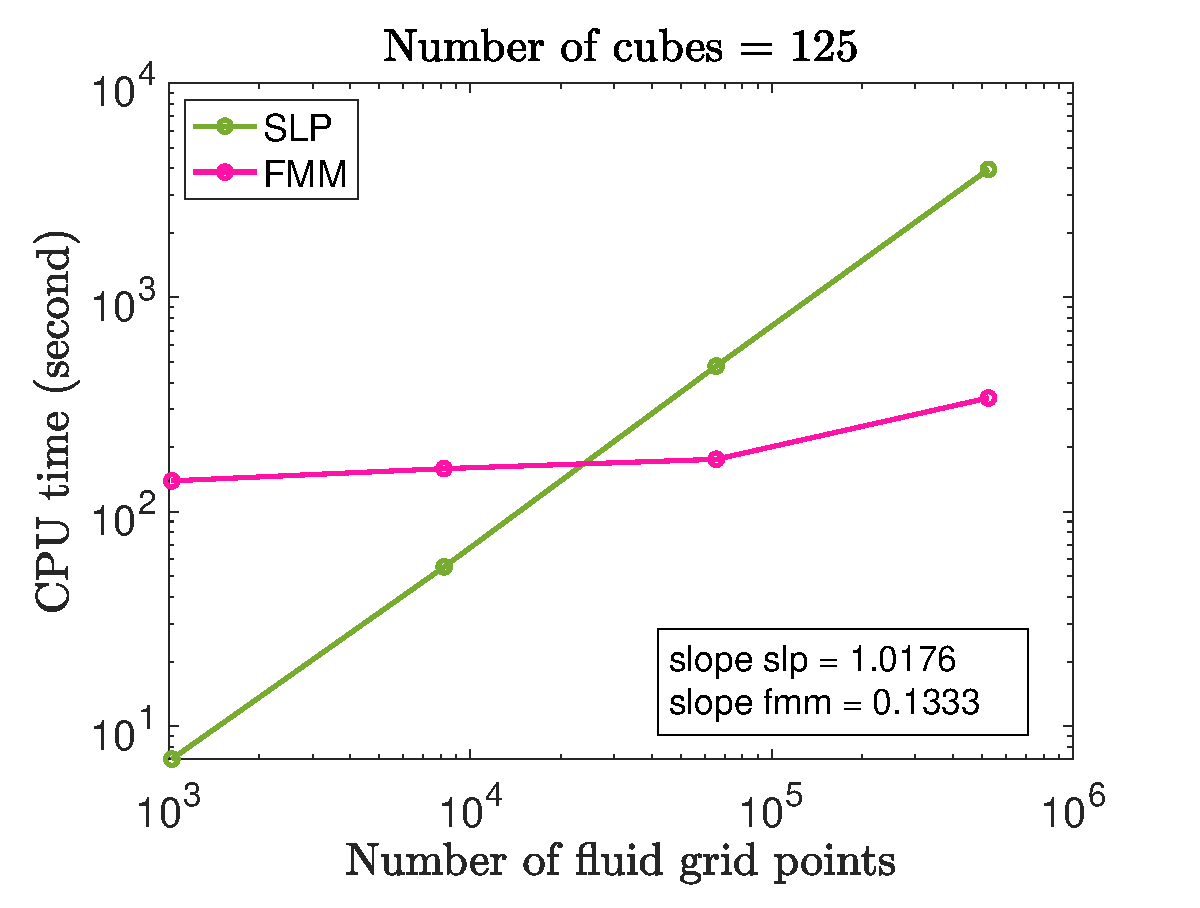
\includegraphics[scale=0.4]{./figures/fig_time_both_mm5_Nt10}
	\caption{CPU time with an aggregate made with 125 cubes for ten time steps. The green line is the velocity computation with the original single-layer potential code, and the pink line represents the approximation using the FMM3D library.}
	\label{fig_vel_mm5_t1}
\end{center}
\end{figure}

%Rotation==============================================
\subsection{Rotation}
To have more realistic simulations, we allow our model aggregates to rotate while they settle.
We here focus on the angular velocity, $\vec{\Omega} = \Delta \theta / \Delta t$, which tells us how much the aggregate rotates ($\Delta \theta)$ in one time step, $\Delta t$. 
\begin{figure}[ht]
	\begin{center}
		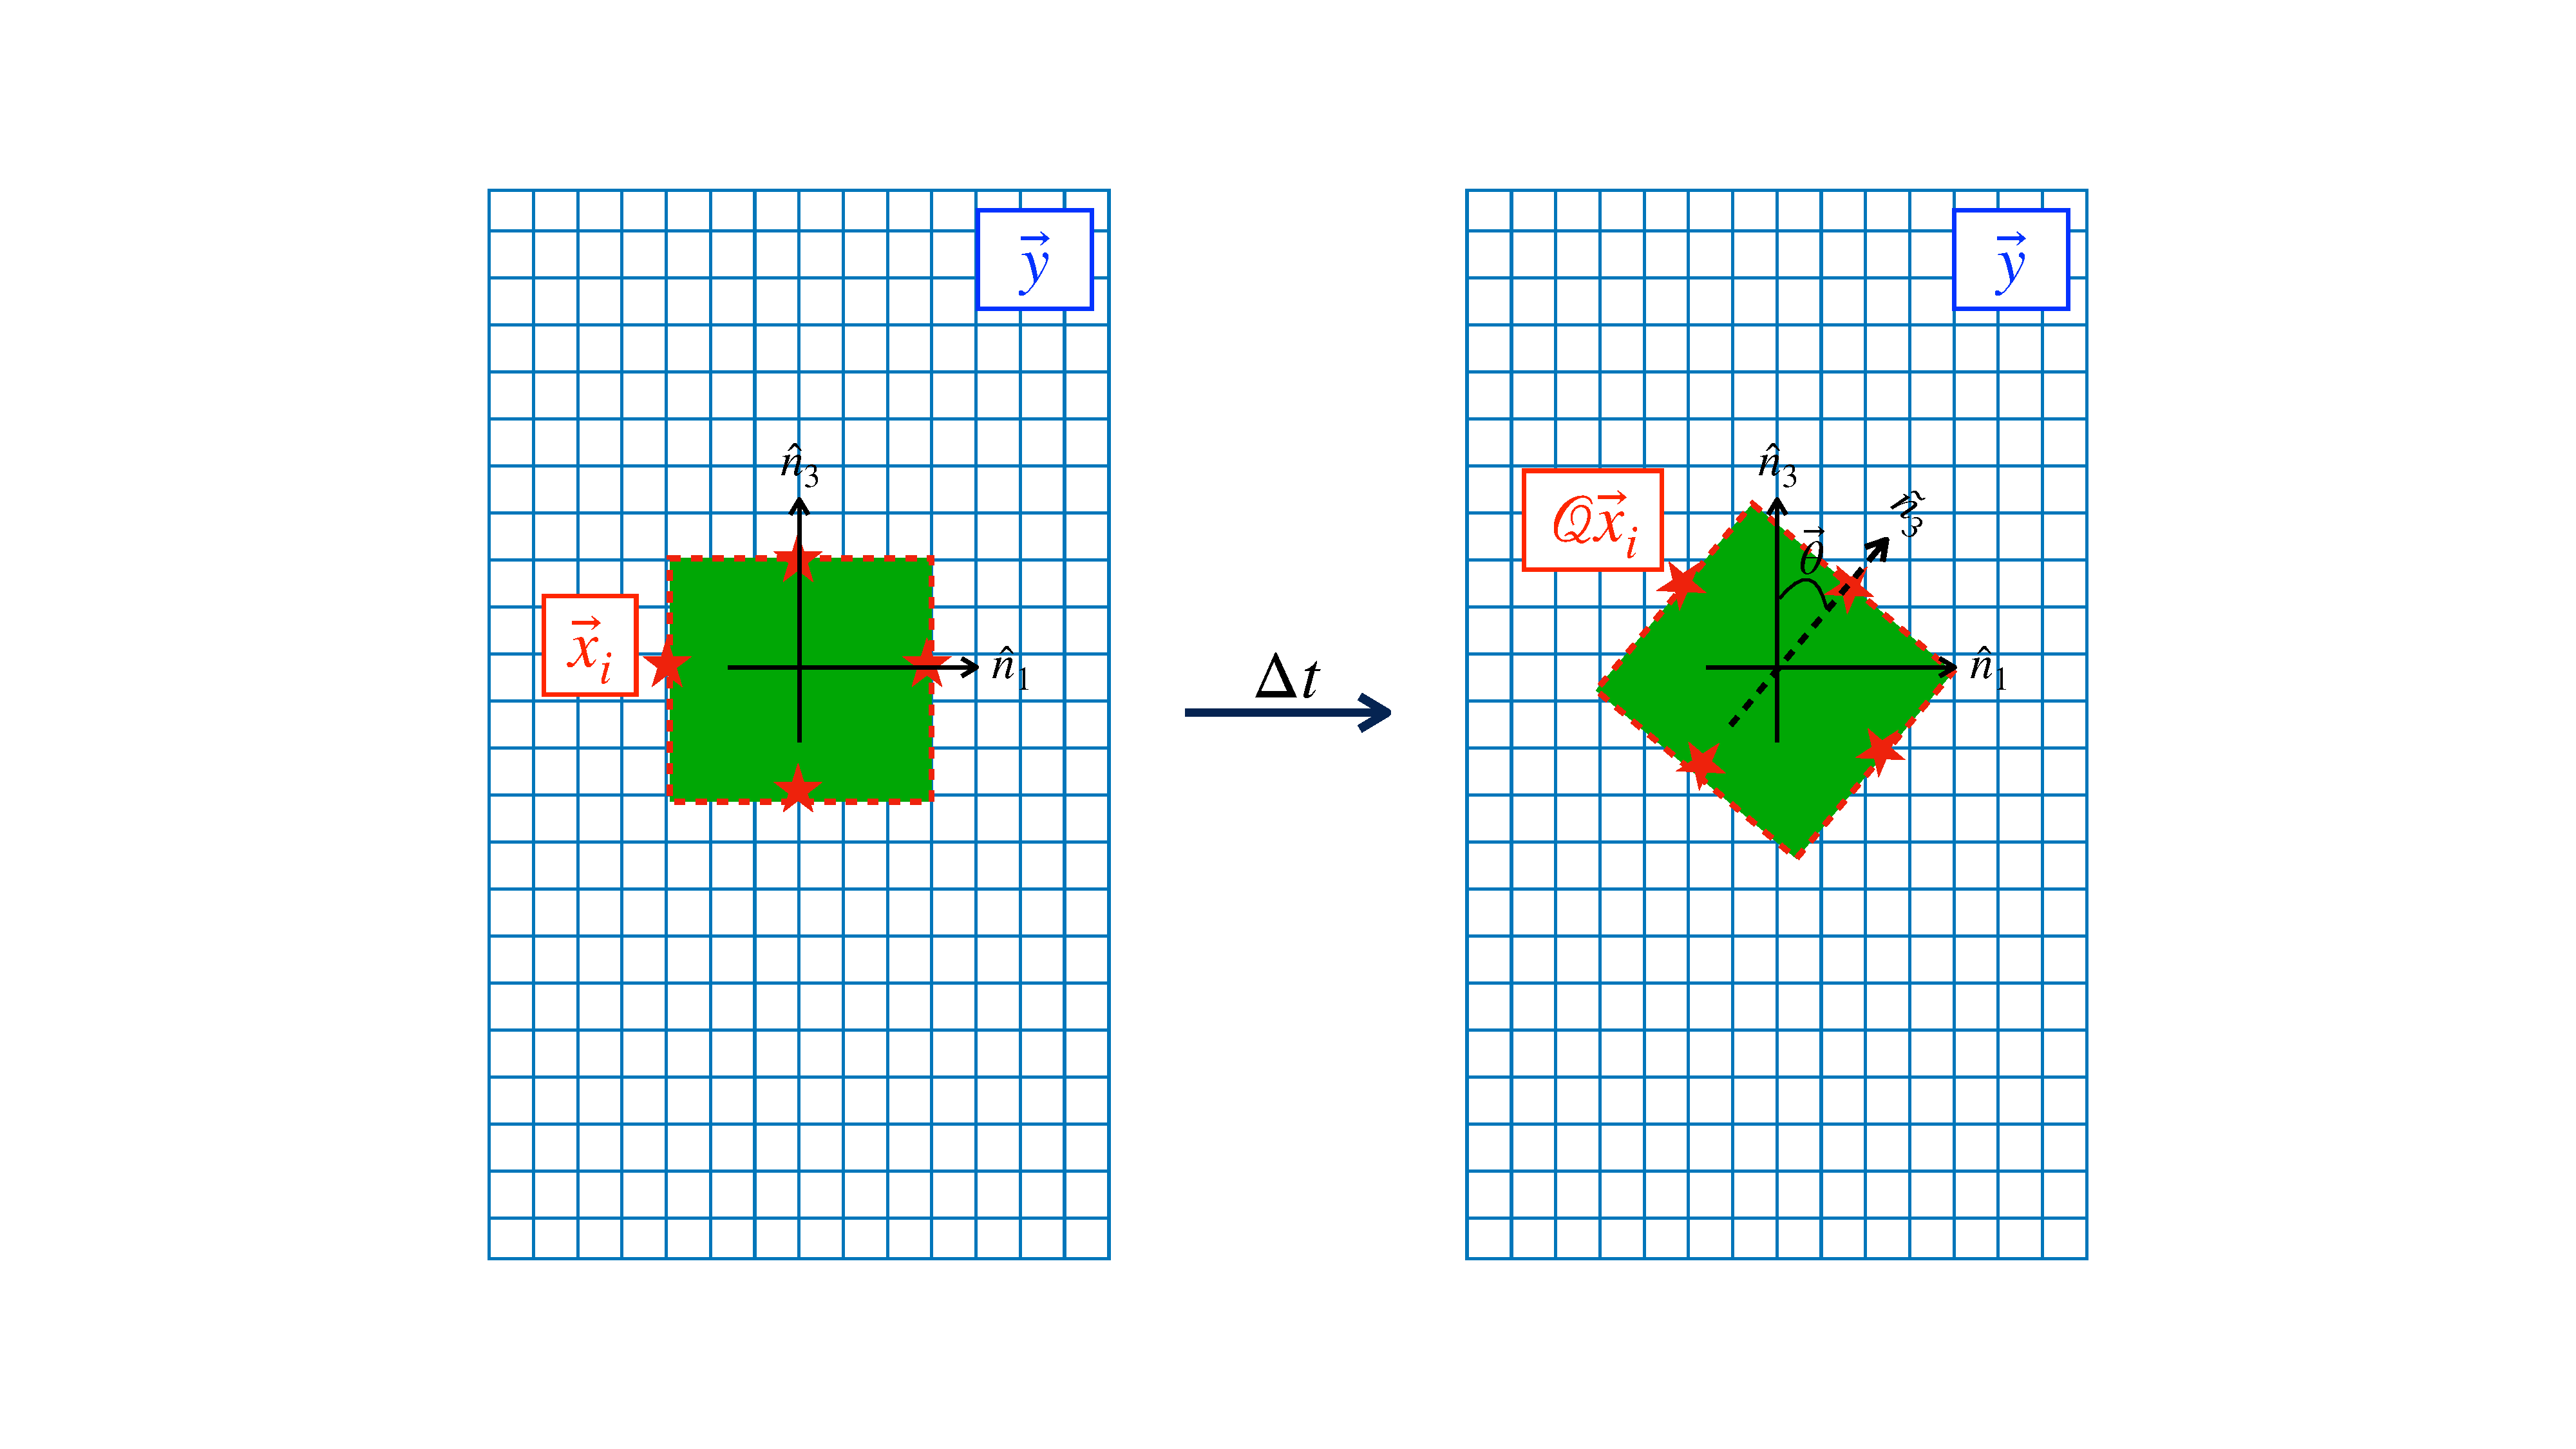
\includegraphics[scale=0.25]{./figures/fig_rotation_schematics.pdf}
	\caption{Schematics of the rotation of an aggregate. The blue grid is the fluid domain and the green rectangle represents an aggregate. Red stars show points on the aggregate.}
	\label{fig_rotation_schematics}
\end{center}
\end{figure}
This information is stored in the orientation matrix, $\mathcal{Q}(t)$. 
We can compute the position, $x_R(t)$ of a point of the surface of the rotated aggregated using
\[
\vec{x}_{\mathcal{R}}(t) = \mathcal{Q}(t) \vec{x}_a,
\]
where $\vec{x}_a $ is the position of a point of the aggregate surface relative to the center of mass expressed in a coordinate system that rotated with the aggregate. We note that $\vec{x}_a$ is constant in time and $\mathcal{Q}(0) = \bar{\bar{I}}$ (identity matrix) initially. After we move forward one time step, we may update this orientation matrix as 
\begin{equation}
	\mathcal{Q}(t + \Delta t) = \mathcal{R} \mathcal{Q}(t),
\end{equation} 
where $\mathcal{R}$ is a rotation matrix. 
\par
We implement updates to the orientation matrix as follows~\cite{polimeno_toward_2022}.
Assume we obtain the angular velocity, $\vec{\Omega}$, from solving equation (\ref{eq_slp_linear_system}) at every time step. (Initially, it is the zero vector). With this, we can find the three-dimensional change of angular position vector, $ \vec{\Omega} \Delta t = \left( \Delta \theta_1, \ \Delta \theta_2, \ \Delta \theta_3 \right) \equiv \Delta \vec{\theta}$.
The matrix $\mathcal{A}$ is then defined such that $\mathcal{A} \vec{x} = \Delta \theta \times \vec{x}$,
\begin{equation}
	\mathcal{A}
	=\begin{bmatrix}
	 0 & - \Delta \theta_3 & \Delta \theta_2  \\
	 \Delta \theta_3 & 0  & -\Delta \theta_1  \\
	 - \Delta \theta_2 & \Delta \theta_1 & 0  \\
	\end{bmatrix},
	\label{eq_rotation_mx}
\end{equation}
From here, we have the rotation matrix $\mathcal{R} = e^{\mathcal{A}}.$
We can compute the matrix exponential $e^{\mathcal{A}}$ using Rodrigues' formula, for antisymmetric matrices
\begin{equation}
	\mathcal{R} = 
e^{\mathcal{A}} 
 = \bar{\bar{I \ }} 
 + \frac{\sin(\phi)}{\phi} \mathcal{A}
 + \frac{1-\cos(\phi)}{\phi^2} \mathcal{A}^2,
\label{eq_R_eA}
\end{equation} 
where $\phi = \|\Delta \vec{\theta}\|_2$.
With this $\mathcal{R}$ and orientation matrix $\mathcal{Q}$, we are ready to update the fluid grid.


	
\subsubsection{Linear system in a rotated coordinate}
We first solve for the stress at the center of each square face of an aggregate, $\vec{y} = \vec{x}_i$, 
using the same formula as equation (\ref{eq_vel_all_onS_nonD}),
\begin{equation}
	\vec{u} \left(\vec{x}_i \right) 
		  = -\int_{S}  
		 \vec{f}(\vec{x}) 
		 \cdot \bar{\bar{G \ }} (\vec{x}, \vec{x}_i) 
		 \ \textrm{d}S 
		 - \frac{ \alpha C_{max}}{8\pi } \frac{\rho_0}{(\rho_s - \rho_0)(1-\phi)}
		 \int_V  C \left(\vec{x} ,t \right) \hat{k} \cdot
		 \bar{\bar{G \ }}(\vec{x}, \vec{x}_i)
		 \ \text{d}V,
		 \nonumber
\end{equation}
As we allow rotation, we can express the above equation as in a rotated frame of reference using $\vec{x}_{r, i} = \mathcal{Q} \vec{x}_i, \ \vec{u}_r = \mathcal{Q} \vec{u}$, and $\vec{f}_r = \mathcal{Q} \vec{f}$
\begin{align}
	\vec{u}_r(\vec{x}_{r, i}) =
	\mathcal{Q}
	\vec{u} \left(\mathcal{Q} \vec{x}_i \right) 
		  = & - \frac{1}{8 \pi} \int_{S}  
		 \vec{f}_r(\mathcal{Q} \vec{x}) 
		 \cdot \bar{\bar{G \ }} (\mathcal{Q} \vec{x},\mathcal{Q}\vec{x}_i) 
		 \ \textrm{d}S
		 \nonumber \\
		 & - \frac{ \alpha C_{max}}{8\pi } \frac{\rho_0}{(\rho_s - \rho_0)(1-\phi)}
		 \int_V  C \left(\vec{x} ,t \right) \hat{k} \cdot
		 \bar{\bar{G \ }}(\vec{x}, \mathcal{Q} \vec{x}_i)
		 \ \text{d}V.
	\label{eq_slp_On_rotate}
\end{align}
Since the rotation matrix $\mathcal{Q}$ is constant in space and is a rotation matrix, it is valid to say that
\[
 \bar{\bar{G \ }} (\mathcal{Q} \vec{x},\mathcal{Q}\vec{x}_i) 
	 = \bar{\bar{G}}( \vec{x}, \vec{x}_i).
\]
We now solve for unknowns, including the translational and angular velocities,
in a rotated coordinate system $\vec{x}_{r,i} $.
Note that the stress values we obtain here 
are located in the rotated positions.  
To complete the linear system to solve for stress, translational, and angular velocities, we temporarily map the fluid domain grid into the same coordinate system as the boundary integral term.
We can multiply by $\mathcal{Q}^{-1} = \mathcal{Q}^{T}$ as 
\begin{align}
	 \vec{u} \left(\mathcal{Q} \vec{x}_i \right) 
		= &
		 -\mathcal{Q}^{-1}
		 \biggl(
		 \frac{1}{8 \pi} \int_{S}  
		 \vec{f}_r(\mathcal{Q} \vec{x}) 
		 \cdot \bar{\bar{G \ }} (\mathcal{Q} \vec{x},\mathcal{Q}\vec{x}_i) 
		 \ \textrm{d}S \biggl)
		 \nonumber \\  
		 & -\mathcal{Q}^{-1}
		 \biggl(
		 \frac{ \alpha C_{max}}{8\pi } \frac{\rho_0}{(\rho_s - \rho_0)(1-\phi)}
		 \int_V  C \left(\vec{x} ,t \right) \hat{k} \cdot
		 \bar{\bar{G \ }}(\vec{x}, \mathcal{Q} \vec{x}_i)
		 \ \text{d}V
		 \biggr).
	\label{eq_slp_vol_R}
\end{align}
For the other force equations as well, we implement the following
\begin{equation}
	\int_{S} \vec{f}(\vec{x}) \  \text{d}S(\vec{x})
	= \mathcal{Q}^{-1} \vec{F}_o
	 \label{eq_drag_code}
	 \end{equation} 
	 \begin{equation}
		 \int_S \vec{f} (\vec{x})  \times (\vec{x} - \vec{x}_{cm}) 
		 \ \textrm{d}S(\vec{x}) 
		 = \vec{0}.
	 \label{eq_torque_code}
	 \end{equation}
Once we solve the linear system, we may return the values on the fluid grid to the Cartesian coordinate system.

\subsubsection{Velocity computation}
Once we solve the stress, we are supposed to use the same 
equation (\ref{eq_vel_all_onS_nonD}) 
to solve for velocity in the fluid grid, which stays in the Cartesian coordinates.
Although the volume integral term can stay as it is,  
the boundary integral needs some special treatment
since it has two mixed coordinate systems.
We particularly pay more attention to the Stokeslet,
\[
	\bar{\bar{G \ }} (\mathcal{Q}\vec{x},\vec{y}) 
	= 
	\frac{\bar{\bar{I \ }}}{||\mathcal{Q}\vec{x}-\vec{y} ||} 
	+ \frac{(\mathcal{Q}\vec{x}-\vec{y})(\mathcal{Q}\vec{x}-\vec{y})^T}{||\mathcal{Q}\vec{x}-\vec{y} ||^3}, 	 
\]
where $\mathcal{Q}\vec{x}$ is in the aggregate rotated grid. Since we cannot compute the boundary integral of the Stokeslet when $\mathcal{Q}\vec{x}$ and $\vec{y}$ are not in the same coordinate system, we need to express $\vec{y}$ using another vector $\vec{v}$ that is in the rotated grid such that 
\[
	\mathcal{Q}\vec{x} - \vec{y} = \vec{x} - \vec{v},
	% \mathcal{Q}\vec{x}-\vec{v} = \vec{x} - \vec{y},
\]
or equivalently,
\[
	\vec{v} = \left(   \bar{\bar{I}} - \mathcal{Q} \right) \vec{x}  + \vec{y}.
\]


After we solve for the velocity field of the fluid domain, we rotate the velocity field back to the original coordinate by multiplying by the inverse of $\mathcal{Q}$ for the concentration update. 
%validation---------------------------------------------------
\section{Validation}
\label{sec:ch3_validation}
As we explained in the previous section, the run time of the entire simulation with an aggregate model using 100 cubes, which we desire to observe, may take up to a few weeks. We thus need to determine the parameters to optimize the computing time, while maintaining an acceptable degree of accuracy. We examine a smaller simulation, using an aggregate with 10 cubes shown in Figure~\ref{fig_sample_agg10}, by varying 1) the $s$ factor for domain size, 2) grid spacing $\Delta x$, and 3) time step  $\Delta t$. Note that we use uniform spacing for all directions, i.e., $\Delta x = \Delta y = \Delta z$. To vary the fluid domain size, we consider the center of mass,  $\vec{x}_{cm}$, and maximum radius, $R_m$, of the aggregate.
We use a domain centered at $\vec{x}_{cm}$ of size  $2s\left[  R_m \times   R_m \times 2 R_m \right]$. We note that $s$ is thus the ratio of the domain size to the aggregate diameter. See Figure~\ref{fig_sample_agg10}.
\begin{figure}[ht]
	\begin{center}
		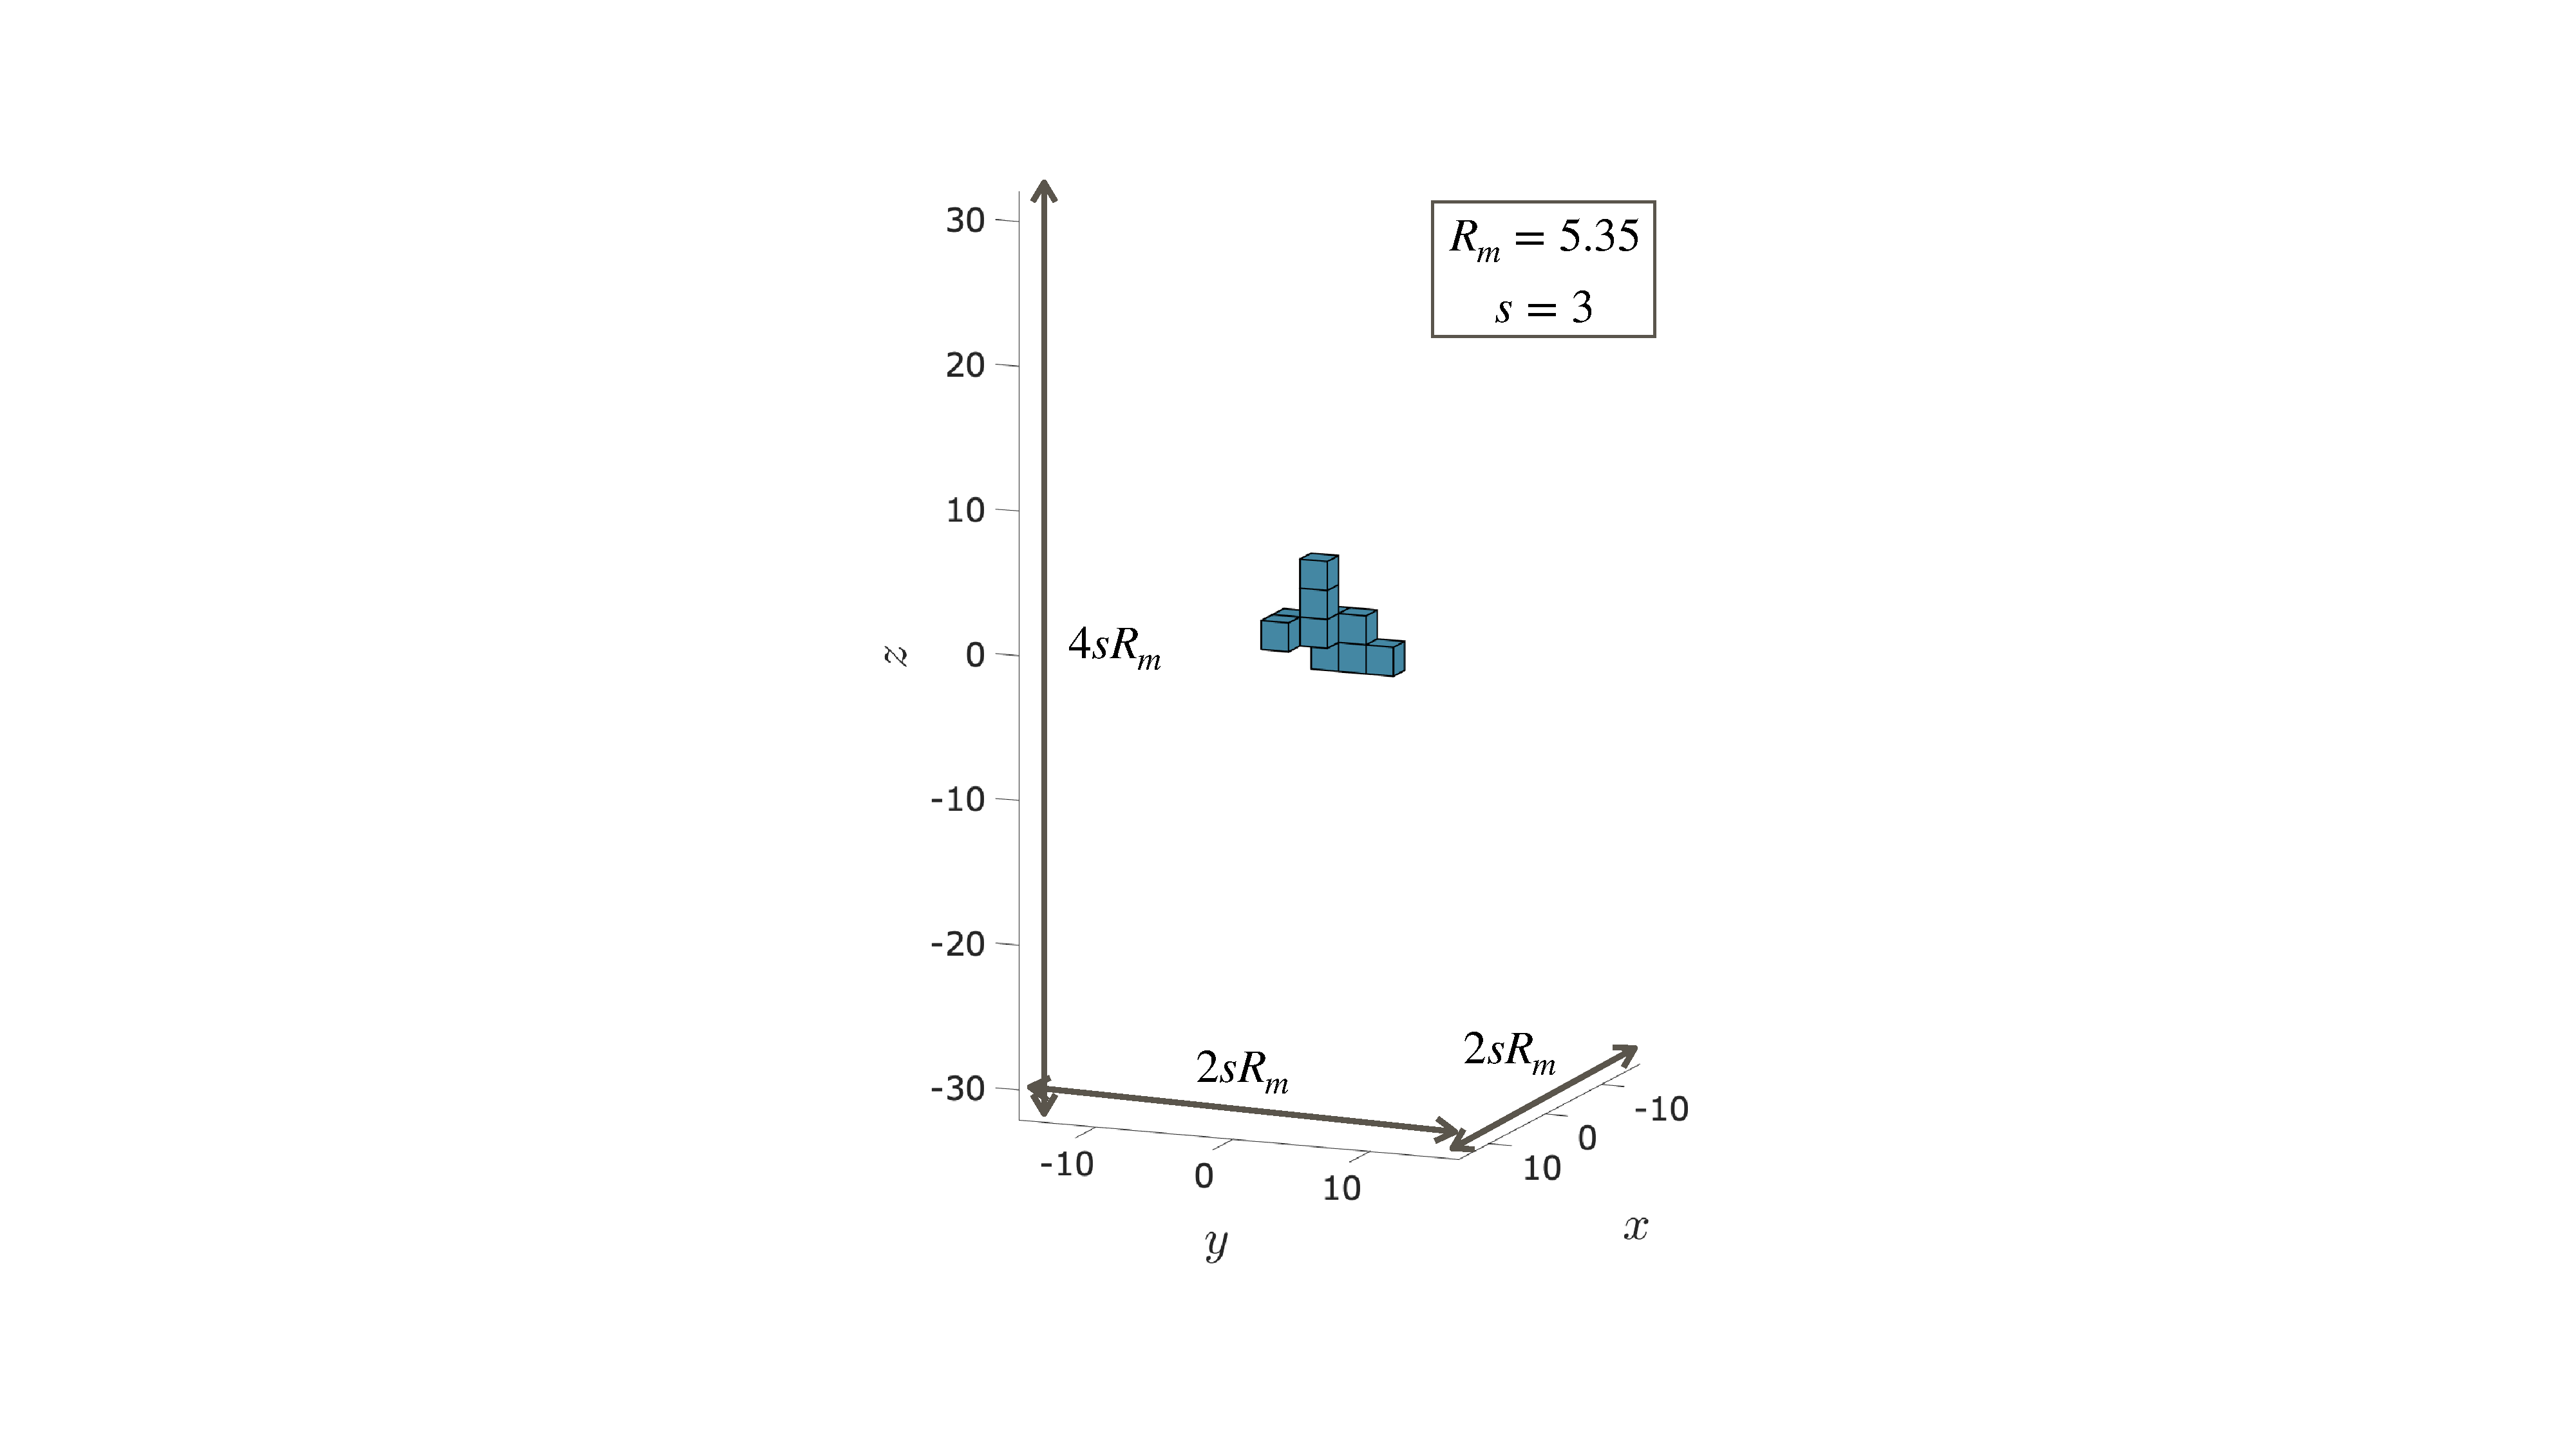
\includegraphics[scale=0.4]{./figures/fig_sample_agg10.pdf}
		\caption{Sample aggregate with ten cubes in a $s=3$ scale domain, that is used to obtain simulations presented in Figure~\ref{fig_NC10_snaps_all}. }
		\label{fig_sample_agg10}
	\end{center}
\end{figure}
\par
Since we are interested in the aggregate's long-term settling behavior, we measure its (a) translational velocity $\vec{U}_a$, (b) location of $\vec{x}_{cm}$, and (c) drag $\vec{F}_o$ as a function of time. 
In particular, we present the vertical component of these three values, focusing on the settling direction.
We also want to observe the (d) perturbation $C(\vec{x},t)$. At locations far from the aggregate, we expect to see very small, almost zero, perturbation.
We thus focus on the perturbation value near the aggregate, denoted by $\vec{x}^{\star}$, which is distanced by approximately $(1.2 + R_m)$ from the center of mass. 
\par
\begin{figure}[ht]
	\begin{center}
		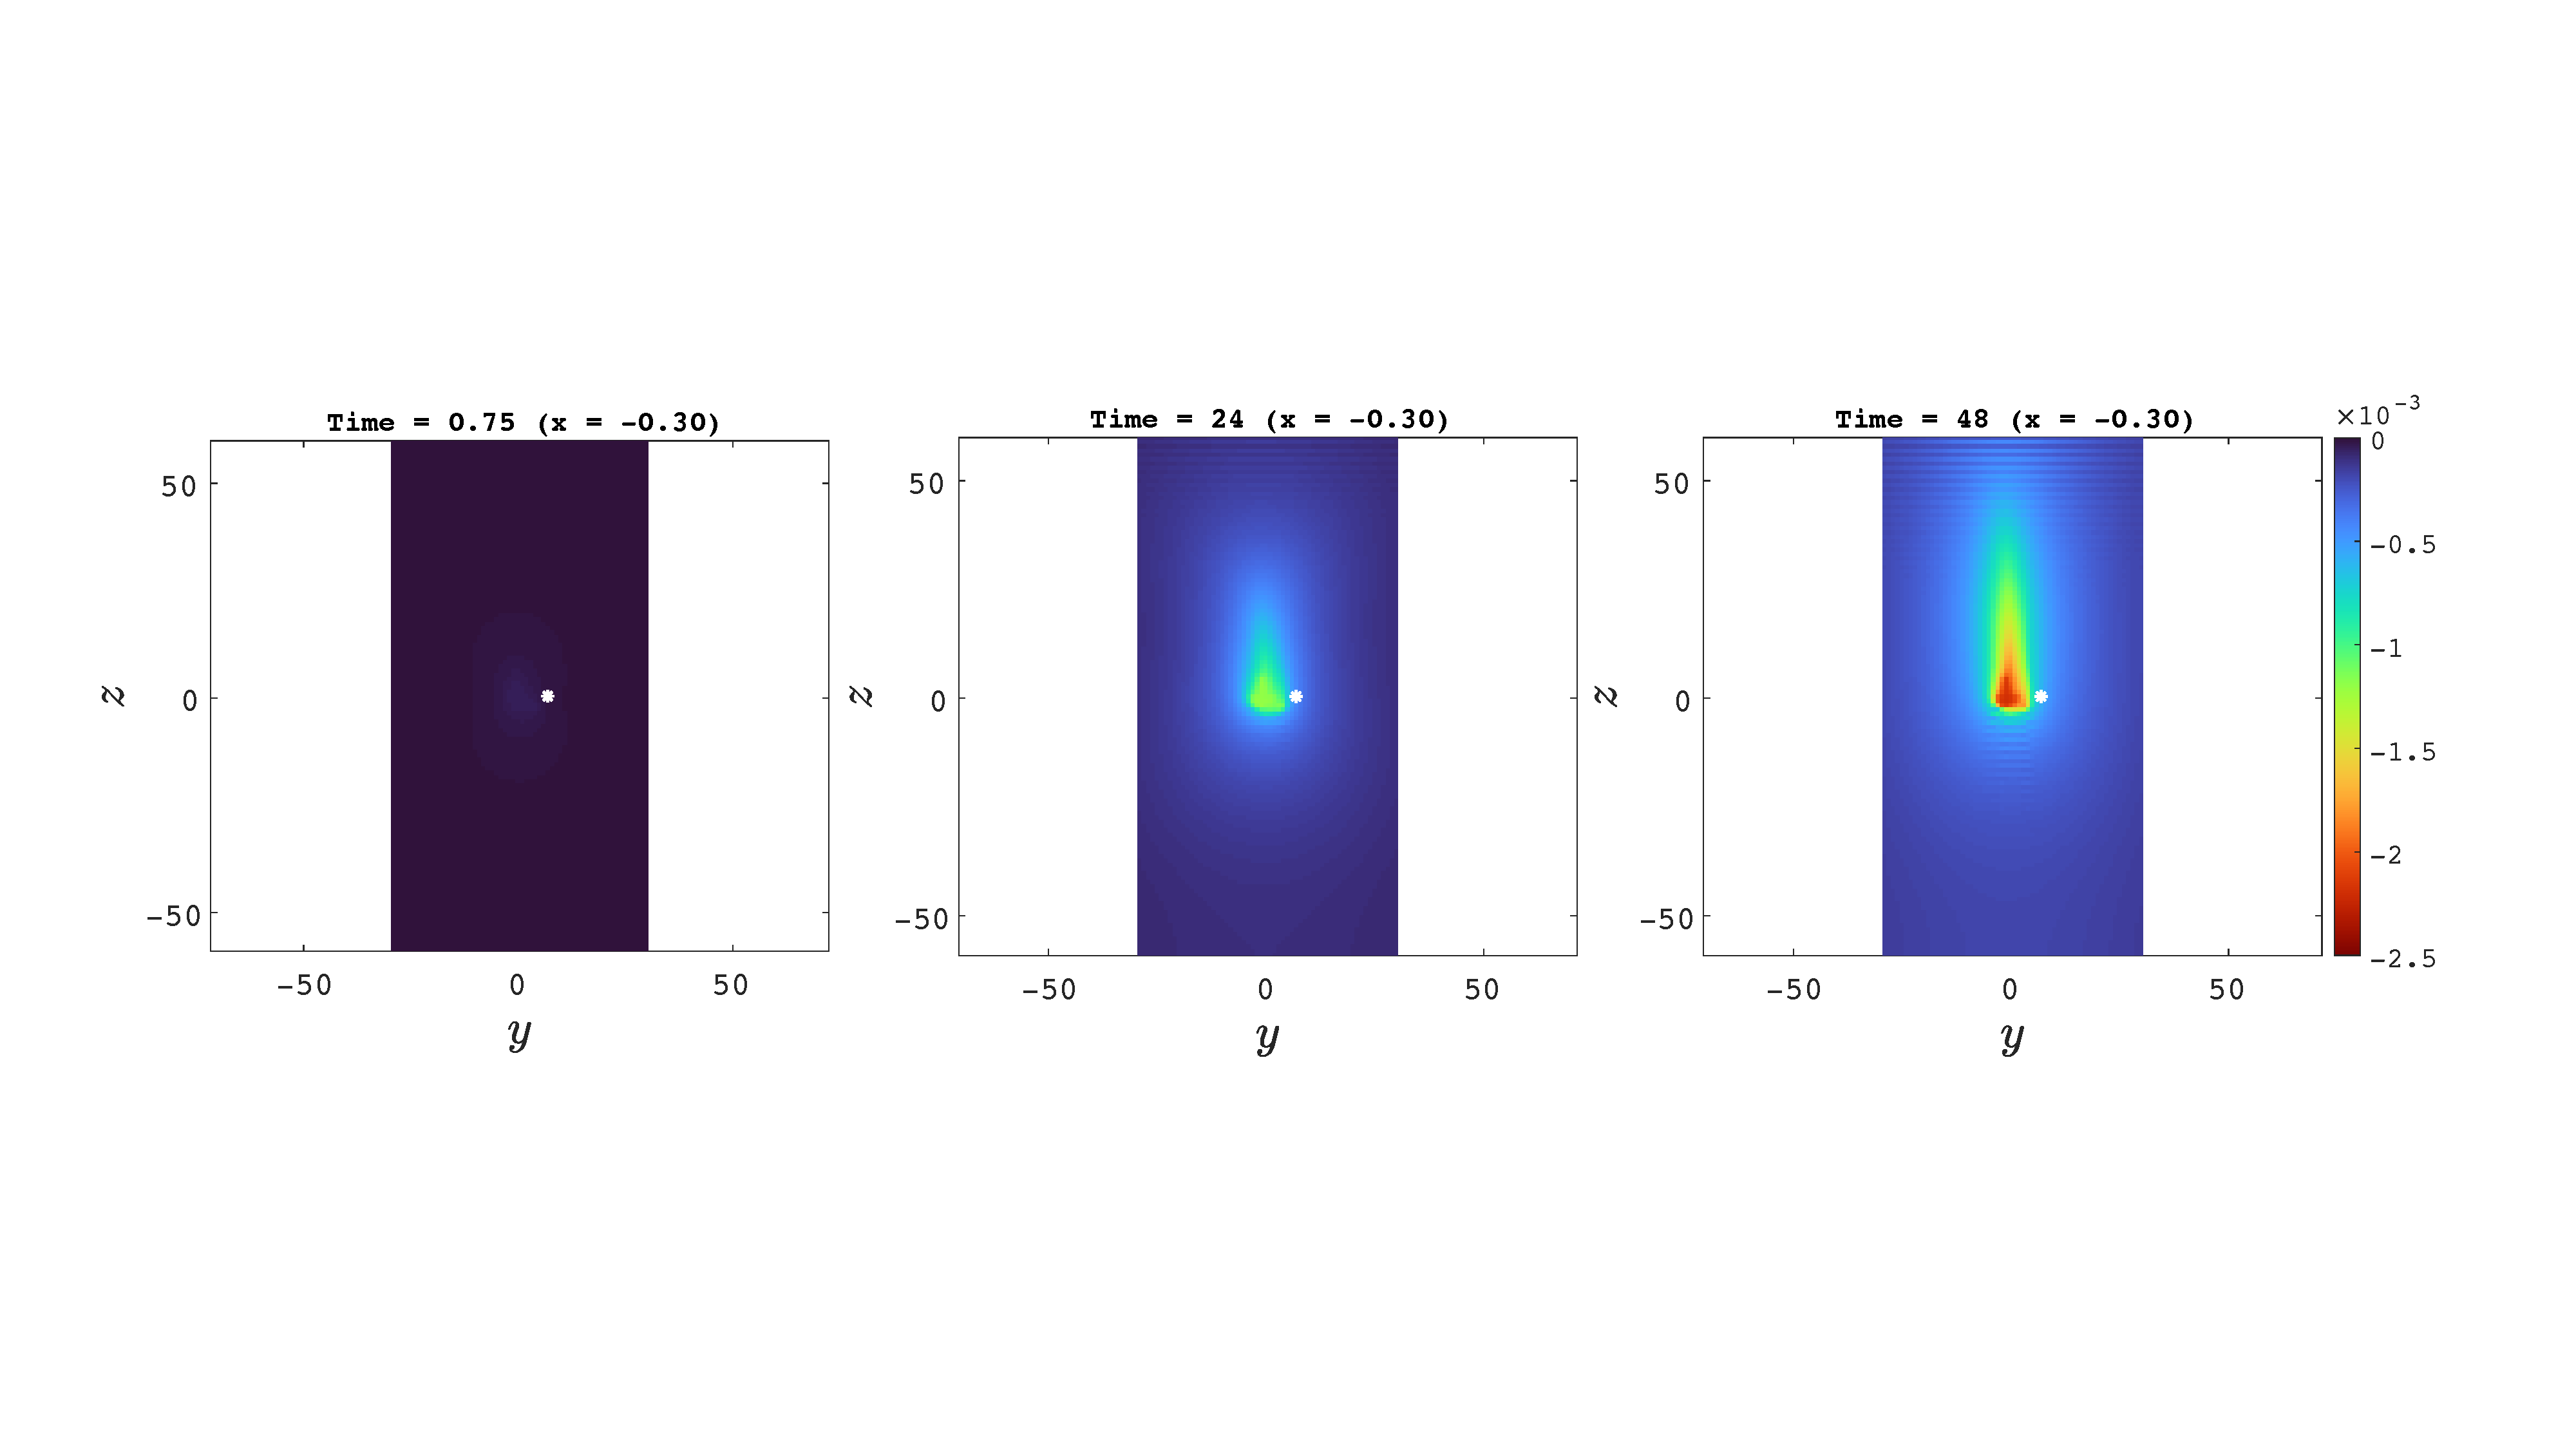
\includegraphics[scale=0.26]{./figures/fig_NC10_snaps_all.pdf}
		\caption{Snapshots of the perturbation obtained with $\Delta t = 0.5, \ \Delta x = 1,$ and $s = 5$. We look at the $y-z$ plane at $x = -0.3$, which is near the center of mass of the aggregate. The small white dot is located outside of, but very close to, the aggregate.}
		\label{fig_NC10_snaps_all}
	\end{center}
\end{figure}
Before we proceed, we show three snapshots of the perturbation $C$ at three different times, obtained with $\Delta t = 0.75, \ \Delta x = 1$, and $s = 5$, at $x = -0.3$ as a sample result in Figure~\ref{fig_NC10_snaps_all}. Note that the white star point is at ${\vec{x}^{\star}} = (-0.3, \    6.9, \      0.4)$, which is the particular point we record $C$. Since we use the moving frame of reference to compute the perturbation, we see that the aggregate stays in the middle of the fluid domain in Figure~\ref{fig_NC10_snaps_all}.
We notice slight oscillations near the top of the fluid domain, where the zero-flux boundary condition is applied, as the perturbation increases. 
However, these oscillations remain relatively small and do not extend to the vicinity of the aggregate. 
Considering a large enough fluid domain compared to the aggregate size, we would like to observe the convergence of the quantities of interest, $\vec{U}_a(t), \ \vec{x}_{cm} (t), \ \vec{F}_o(t)$, and $C(\vec{x}^{\star}, t)$.
\subsection{Varying the domain size, via parameter $s$}
As we described in section~\ref{subsec:AD_numerics_space}, we have periodic boundary conditions on the horizontal plane to model the infinite domain where the velocity vanishes to zero. 
We seek to determine to domain size, via the multiplicative factor $s$, required to approximate these conditions.
If we can obtain good information on the aggregate in a smaller domain, we could use smaller $s$ that results in more rapid computations and smaller memory requirements. 
\begin{figure}[ht]
	\begin{center}
		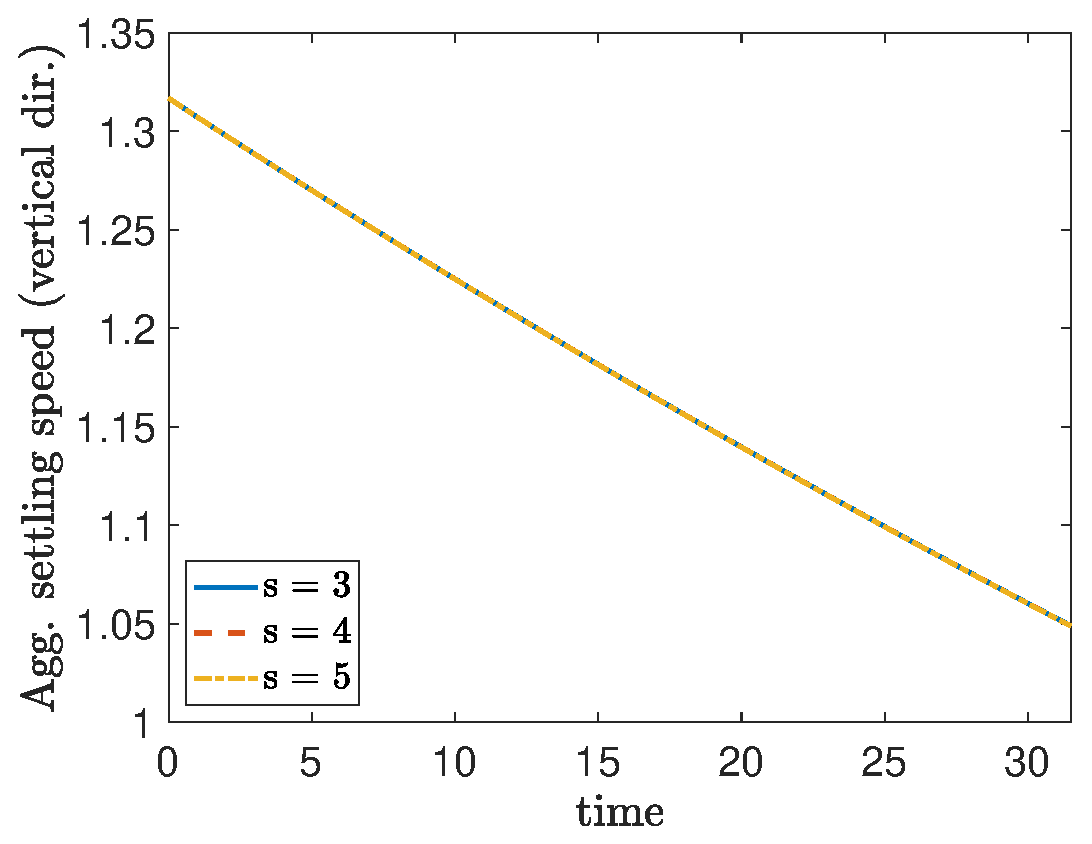
\includegraphics[scale=0.35]{./figures/fig_NC10_s_Ua3_all}
		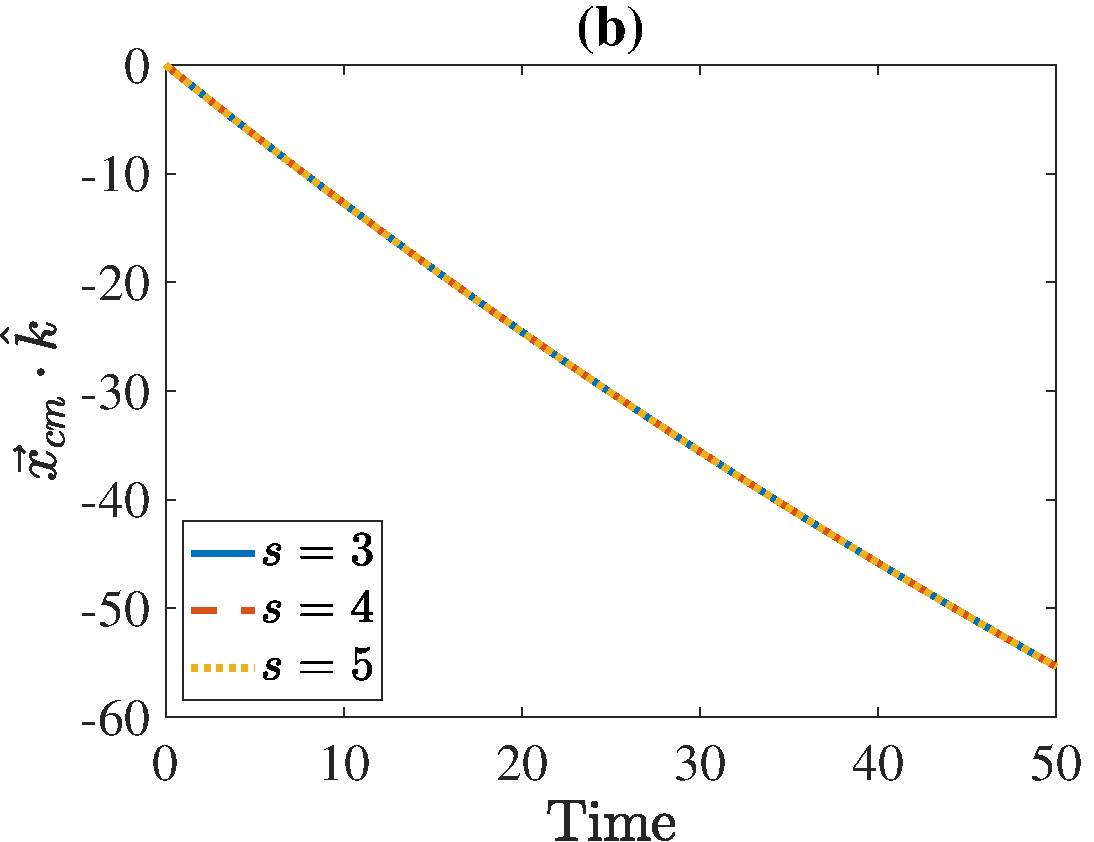
\includegraphics[scale=0.35]{./figures/fig_NC10_s_cm3_all}
		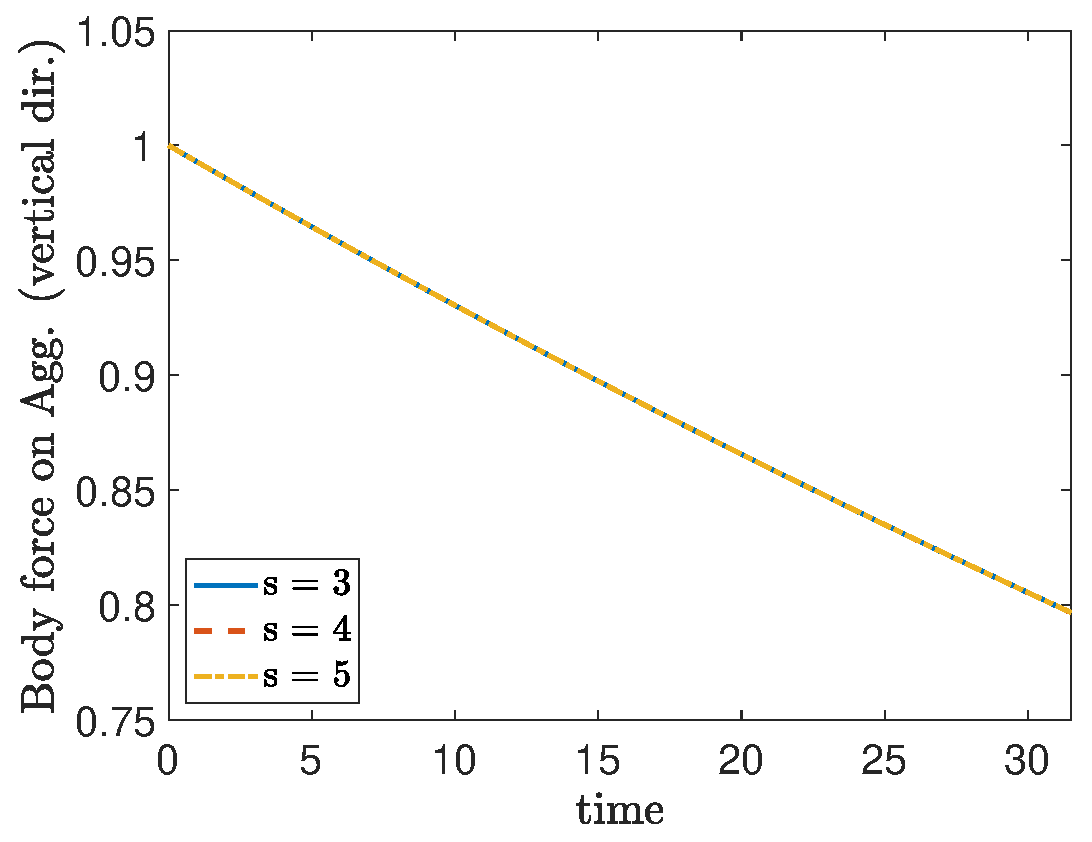
\includegraphics[scale=0.35]{./figures/fig_NC10_s_Fo3_all}
		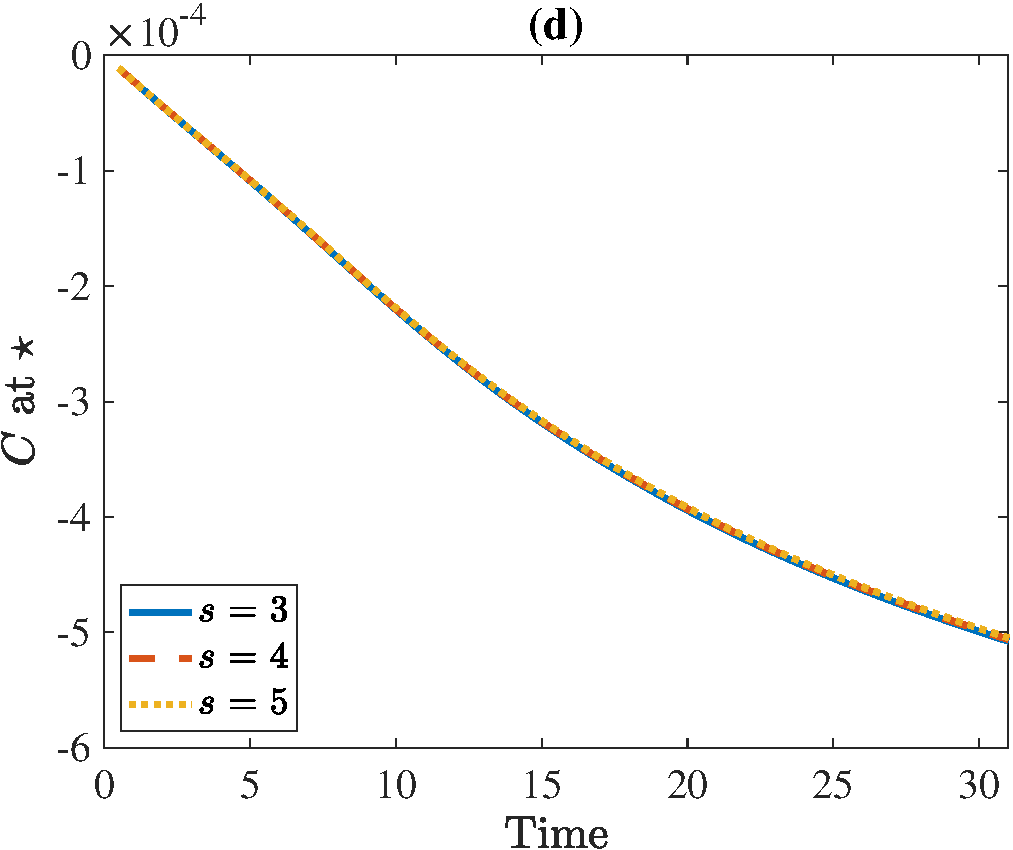
\includegraphics[scale=0.35]{./figures/fig_NC10_s_C_star}
	\caption{Compare various domain sizes with $ s = 3, \ 4, \ 5$ in the time step  $\Delta t = 0.5$ and grid size $\Delta x = 1$. We show (a) the settling speed, (b) the position of the center of mass, (c) the vertical force on the aggregate, and (d) the value of the perturbation at $\vec{x}^{\star}$.}
	\label{fig_NC10_compare_s}
\end{center}
\end{figure}
\par
In Figure~\ref{fig_NC10_compare_s}, we see three different domain sizes with the $s$ factor $s = 3, \ 4$, and $5$. At first glance, we can barely tell the differences between all three cases. In other words, there is no significant impact on aggregate behavior when reducing the domain size down to $s = 3$. Although we notice that the perturbations at $\vec{x}^{\star}$ show a little more variation with $s$, this remains a negligible effect.

\subsection{Varying time step size, $\Delta t$}
We now vary the time step size, $\Delta t$. We consider three different cases, $\Delta t = 0.75, \ 0.5, $, and $0.25$. We are able to run simulations with somewhat large time steps since the aggregate size is small enough to have a velocity of order one. When the initial settling velocity is high, the CFL condition (\ref{eq_CFL}) can be violated, leading to instability. As the aggregate settle, the surrounding fluid becomes denser, which decreases the velocity, and therefore the CFL number. Thus, we care more about the velocities at the beginning of the simulation. 
\par
While we vary $\Delta t$, we set the domain size using domain size to aggregate diameter ratio $s = 3$ since we observed no critical changes in aggregate dynamics and we can save computation time. For a fair comparison, we keep the grid size $\Delta x =1$. 
The main takeaway of Figure~\ref{fig_NC10_compare_dt} is that there are no significant differences in the values we observe. Once again, we notice some variations of the perturbation at later times. 
However, these remain smaller than 4\%.
\begin{figure}[ht]
	\begin{center}
		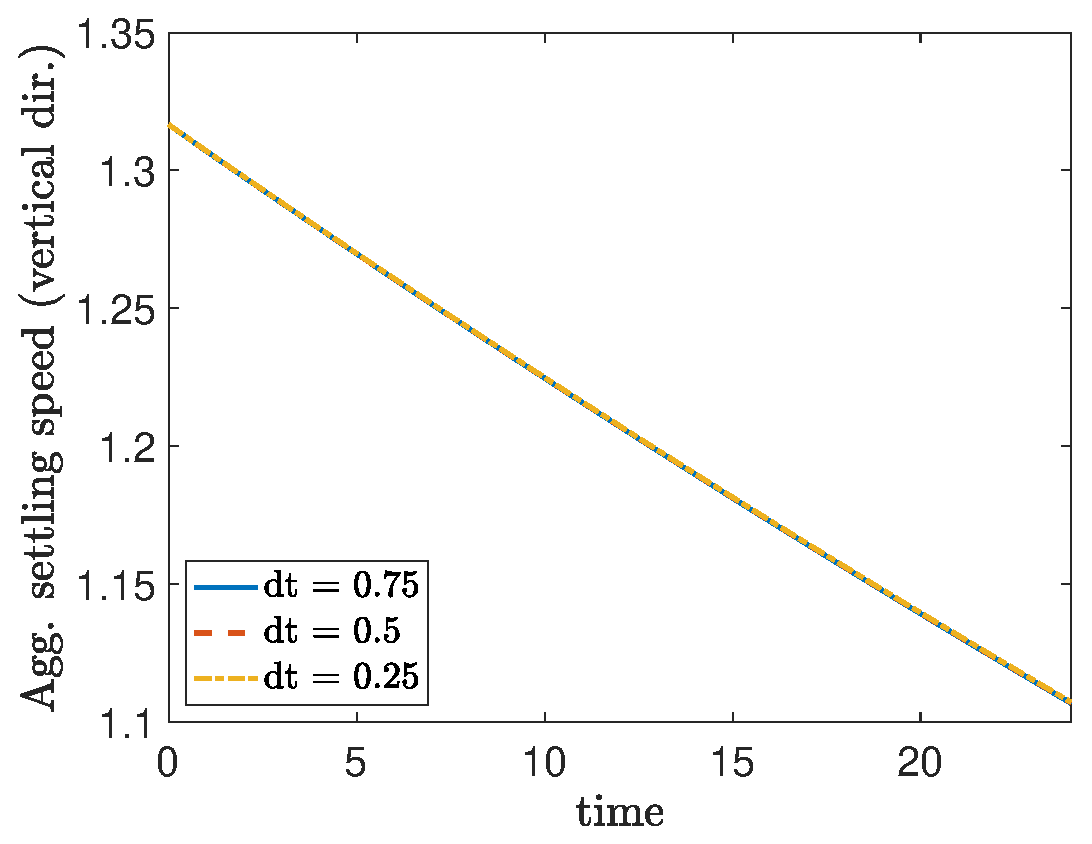
\includegraphics[scale=0.35]{./figures/fig_NC10_dt_Ua3_all}
		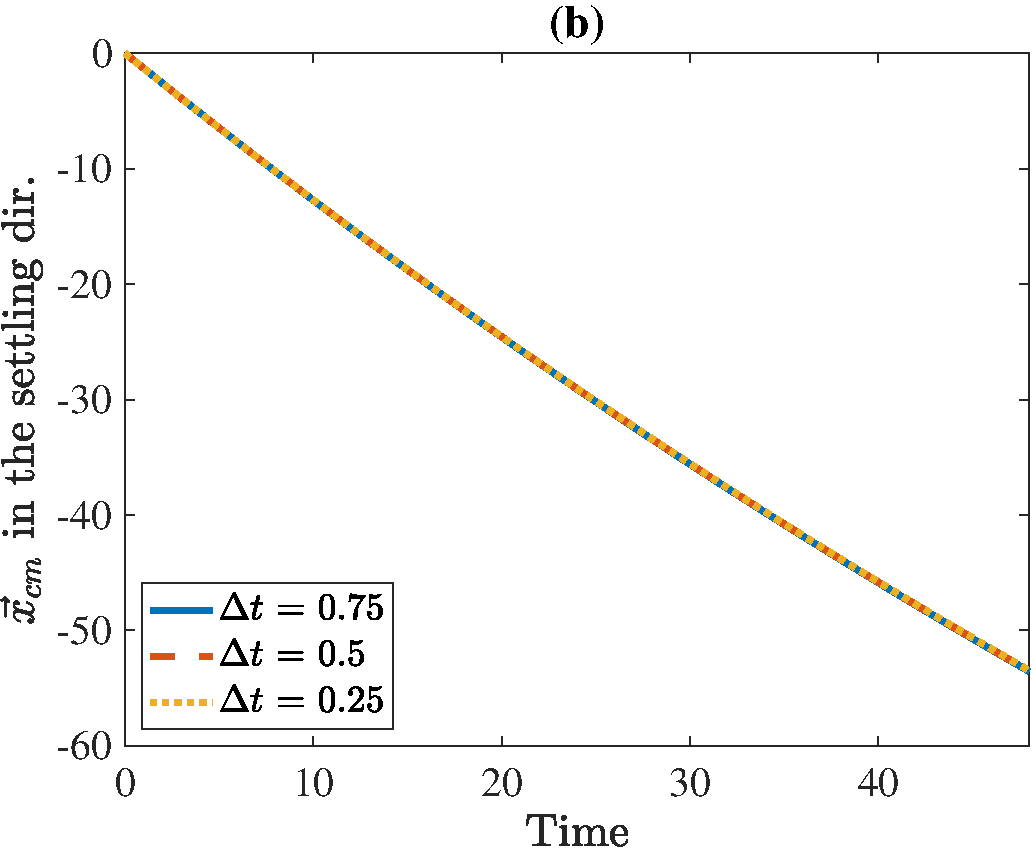
\includegraphics[scale=0.35]{./figures/fig_NC10_dt_cm3_all}
		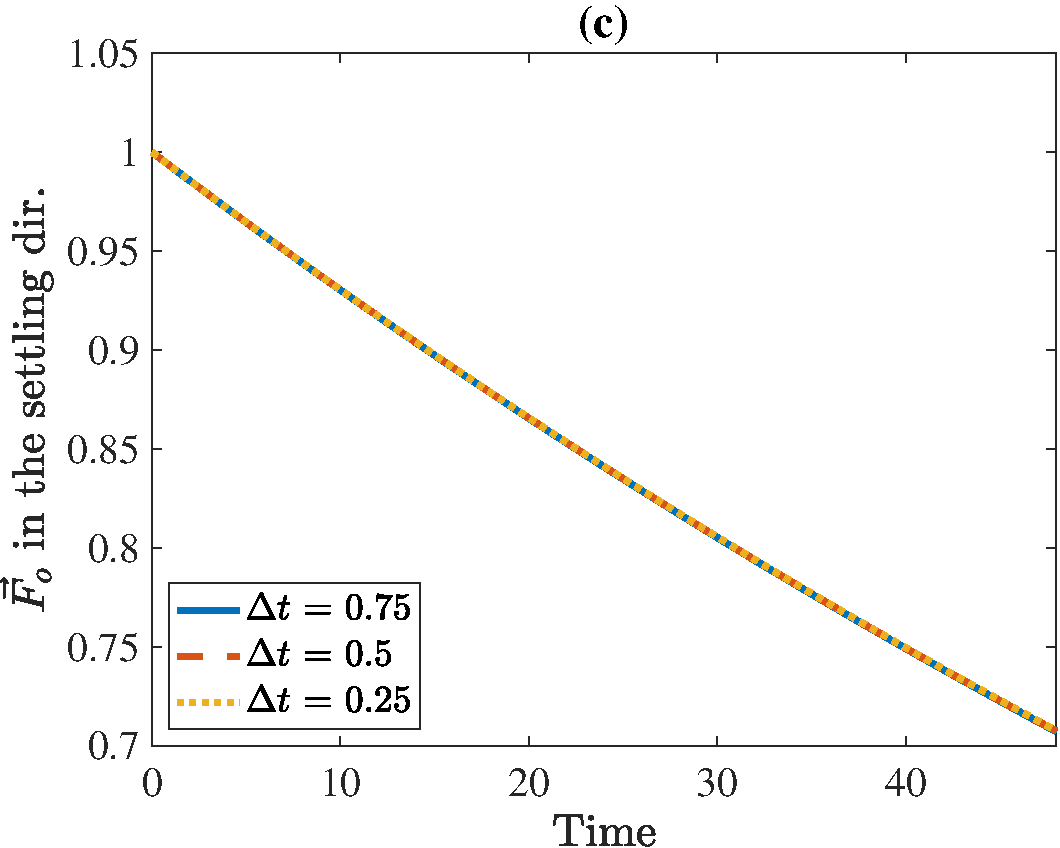
\includegraphics[scale=0.35]{./figures/fig_NC10_dt_Fo3_all}
		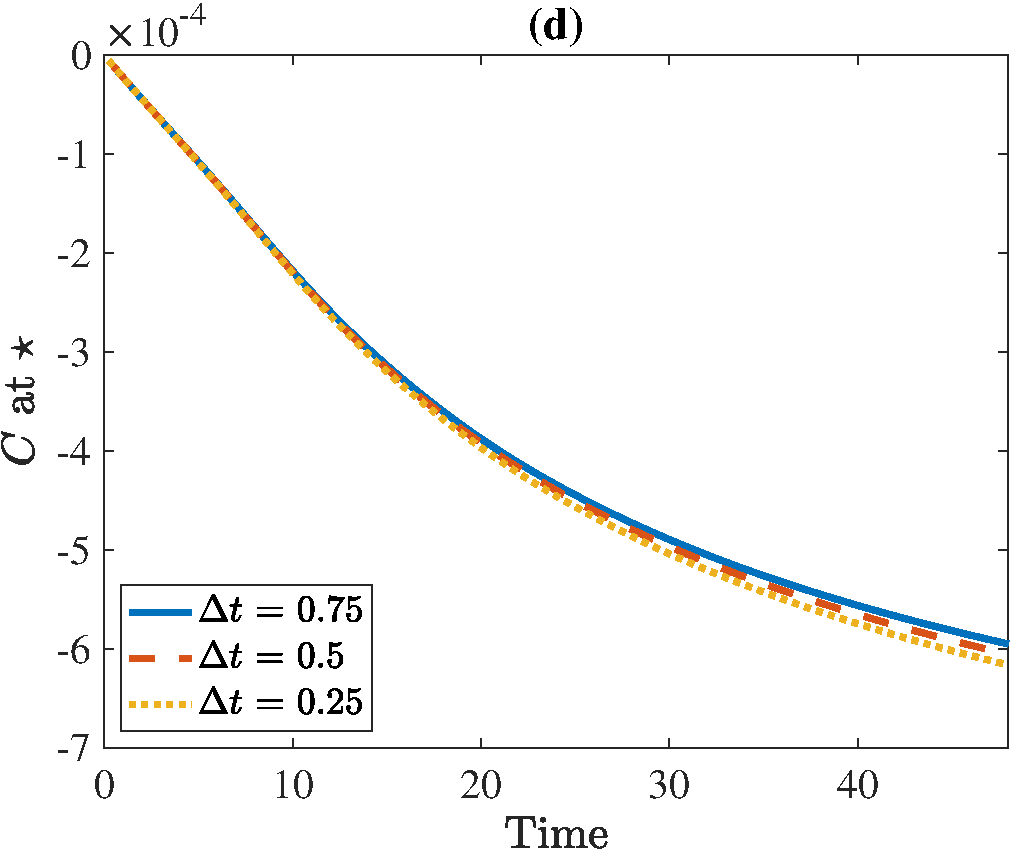
\includegraphics[scale=0.35]{./figures/fig_NC10_dt_C_star}
	\caption{Compare various $\Delta t = 0.75, \ 0.5, \ 0.25$ in the domain size factor $s = 5$ with $\Delta x = 1$. We show (a) the settling speed, (b) the position of the center of mass, (c) the vertical force on the aggregate, and (d)the value of the perturbation near the aggregate.}
	\label{fig_NC10_compare_dt}
\end{center}
\end{figure}
\par
To more accurately capture the effects of varying $\Delta t$, we also present the absolute differences between consecutive two $\Delta t$ cases in Figure~\ref{fig_NC10_dt_err_all}.
It is clear that the errors of all four cases are fairly small compared to the corner error we found in section~\ref{subsec:FMM} (due to the approximation of constant stress over each face). For the time integration scheme we use, which is the explicit RK2 method, we typically expect to have second-order convergence. These error plots support that our solutions already reached convergence.
\begin{figure}[h]
	\begin{center}
		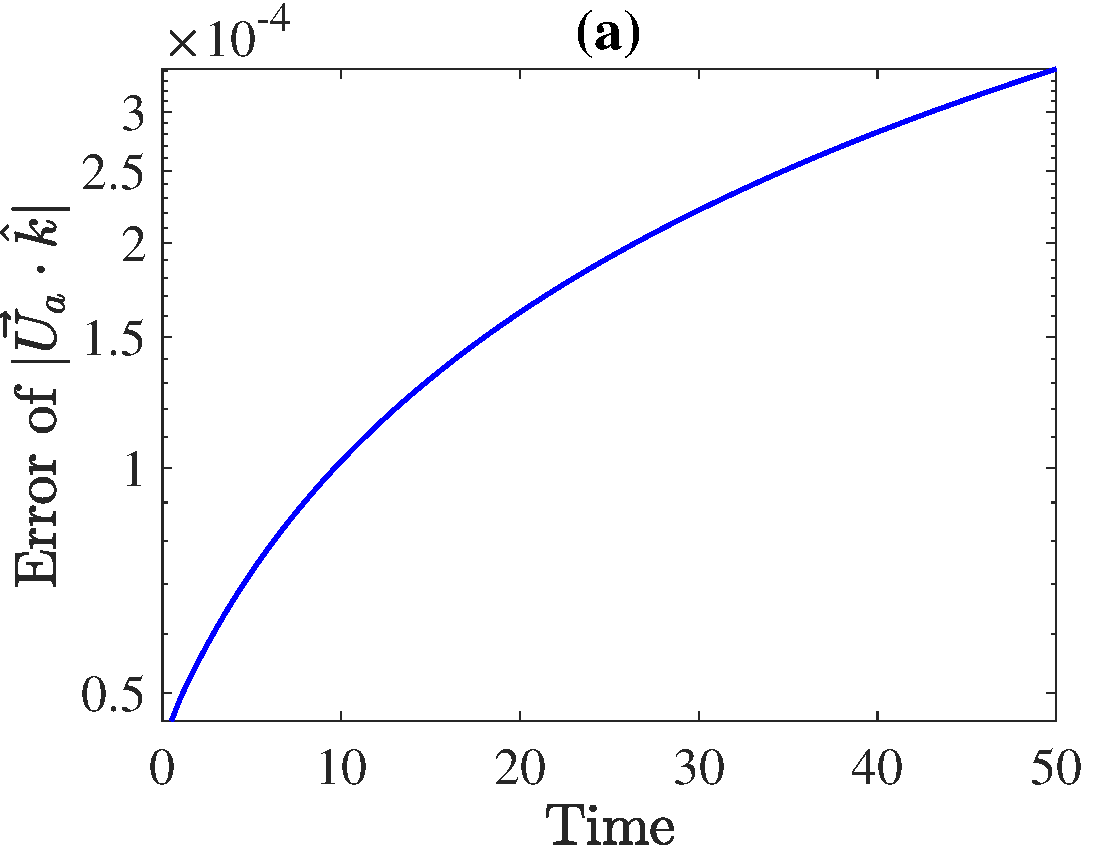
\includegraphics[scale=0.35]{./figures/fig_NC10_dt_err_Ua3_all}
		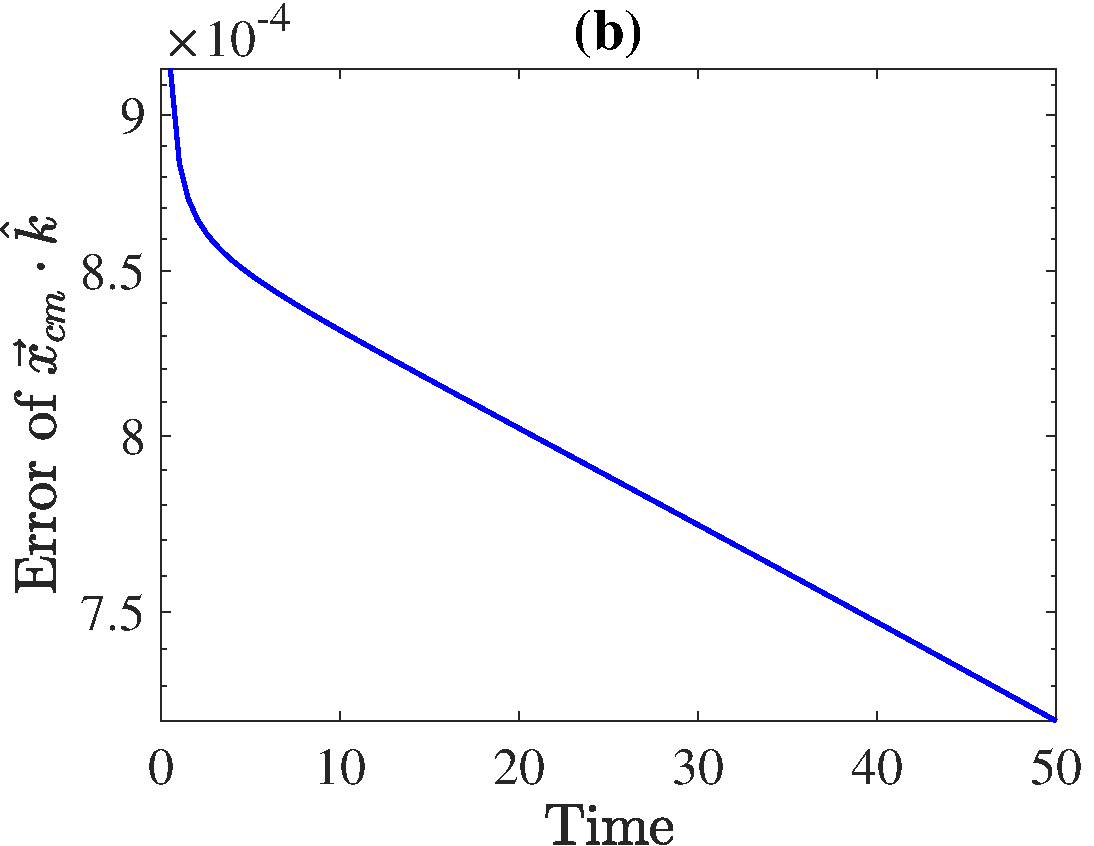
\includegraphics[scale=0.35]{./figures/fig_NC10_dt_err_cm3_all}
		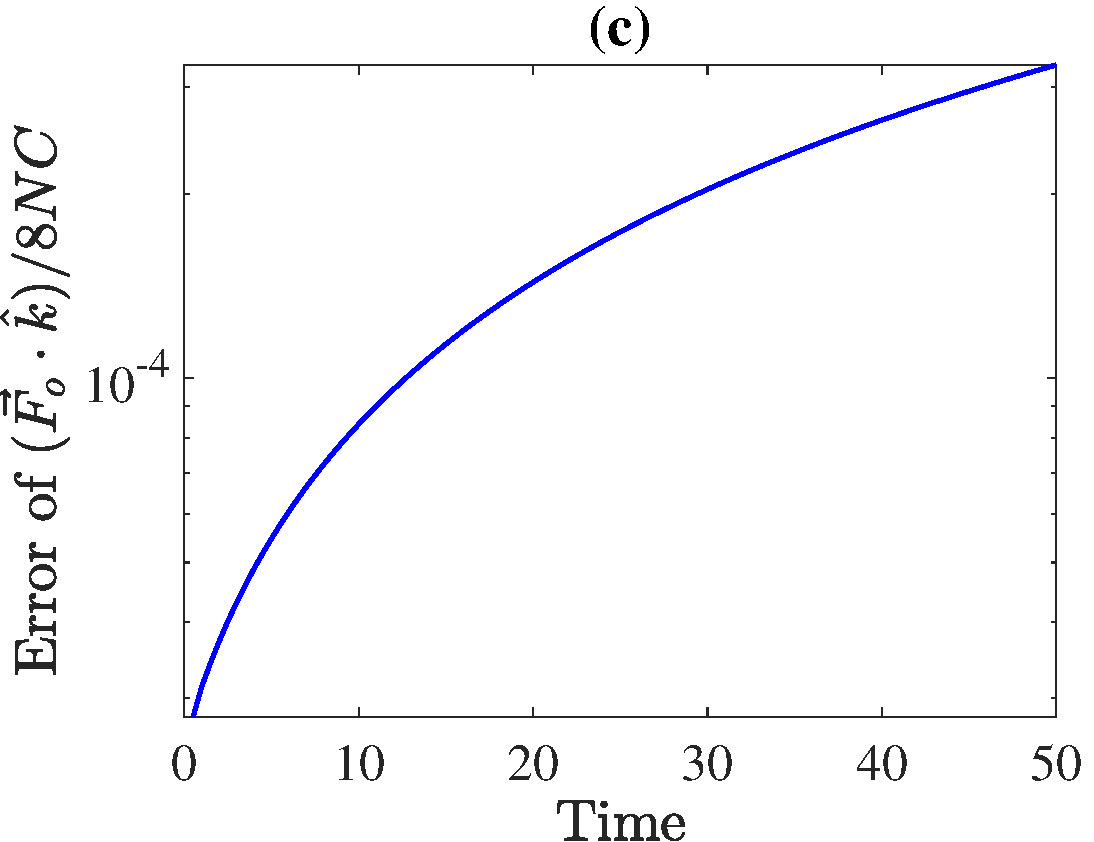
\includegraphics[scale=0.35]{./figures/fig_NC10_dt_err_Fo3_all}
		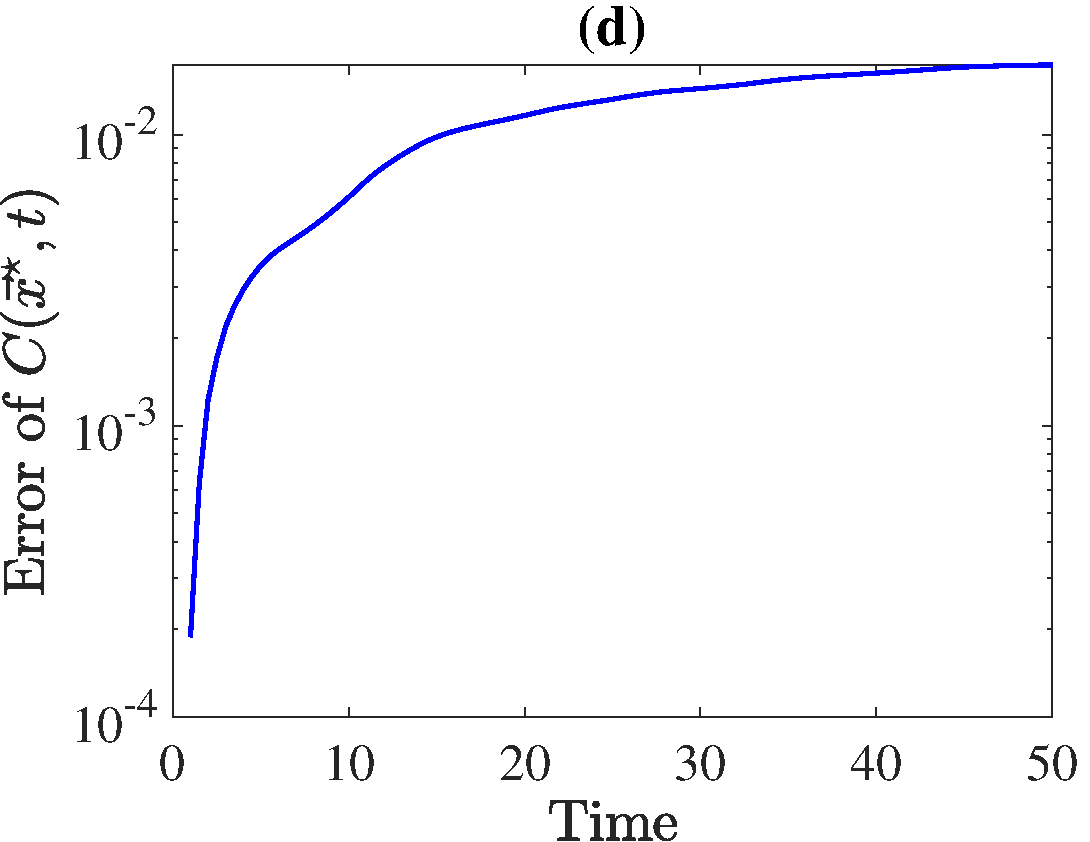
\includegraphics[scale=0.35]{./figures/fig_NC10_dt_err_C_star}
	\caption{Relative error between $\Delta t = 0.5$ and 0.25 cases.}
	\label{fig_NC10_dt_err_all}
\end{center}
\end{figure}

\subsection{Varying grid size, $\Delta x$}
Lastly, we perform the simulations with several grid sizes, $\Delta x = 1, \ 2, $ and $4$. 
The choice of such large grid sizes is justified by the approximation of constant stress over each face (of side length 2).
In general, as long as all three choices produce similar results and have no stability issues, we prefer to use as large $\Delta x$ as possible to reduce the computational time. 
The number of fluid grid points can also be an obstacle in terms of memory. 
\par
\begin{figure}[ht]
	\begin{center}
		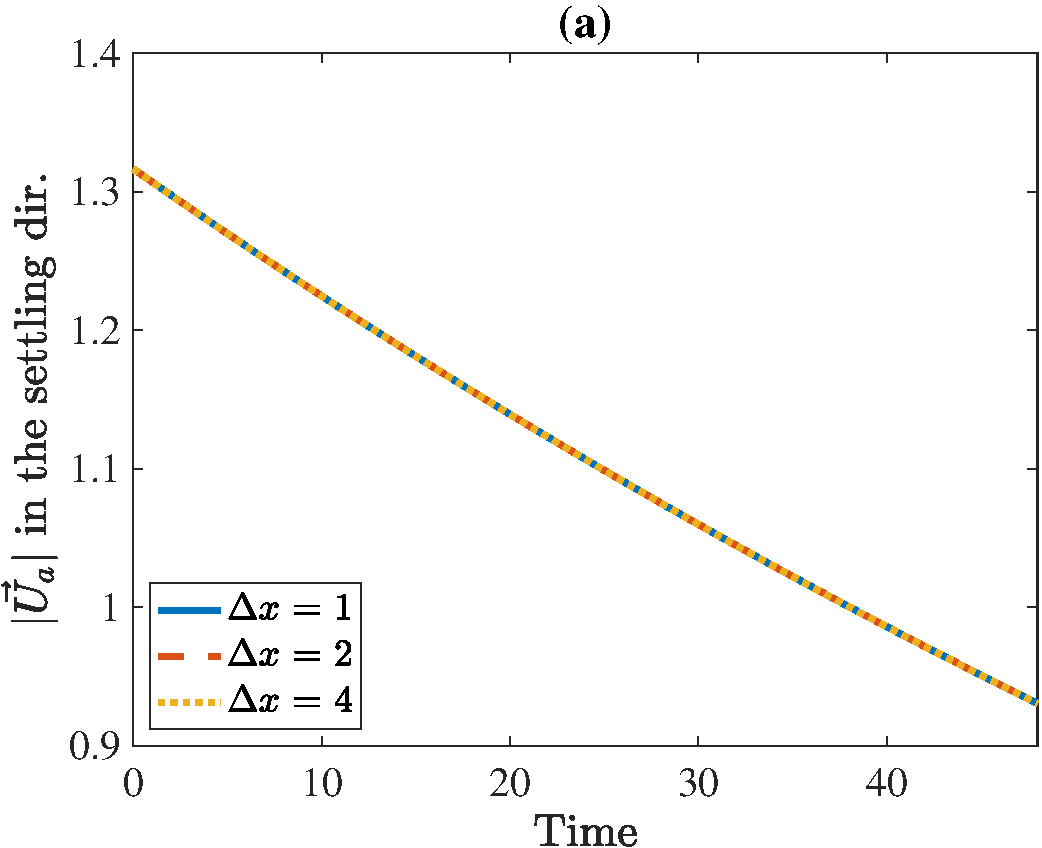
\includegraphics[scale=0.35]{./figures/fig_NC10_dx_Ua3_all}
		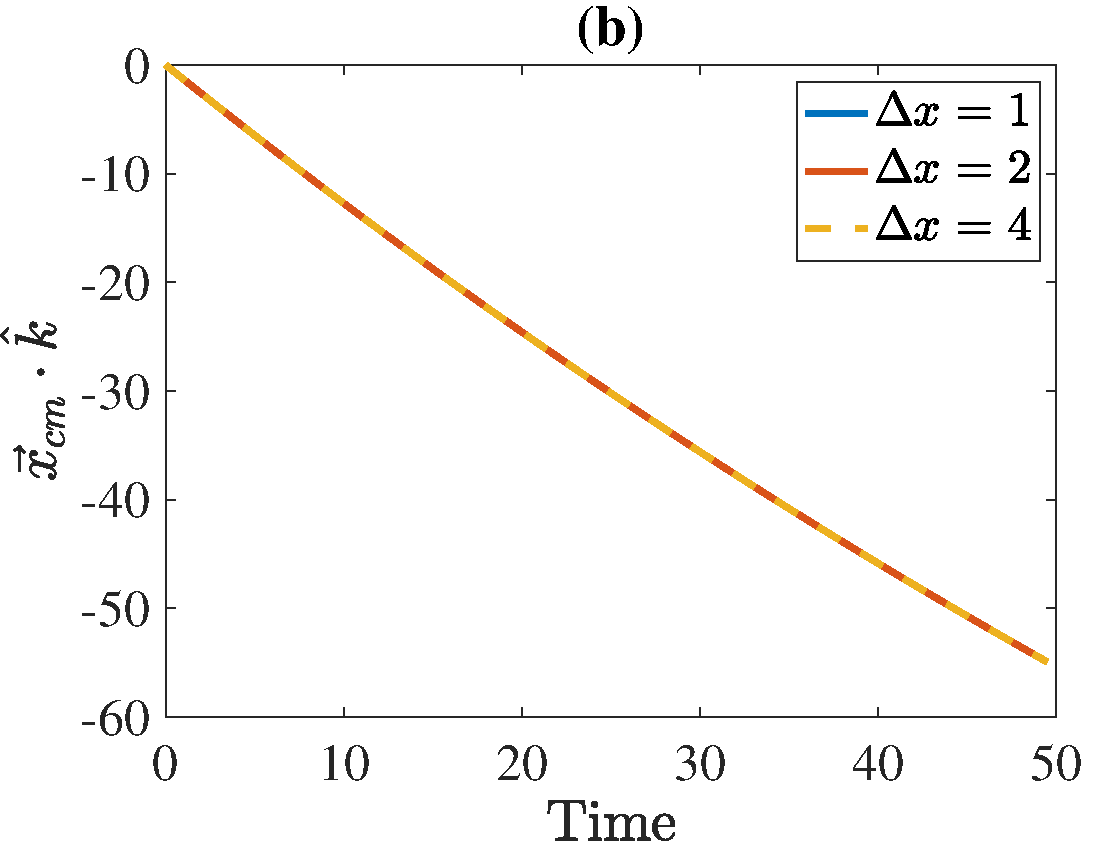
\includegraphics[scale=0.35]{./figures/fig_NC10_dx_cm3_all}
		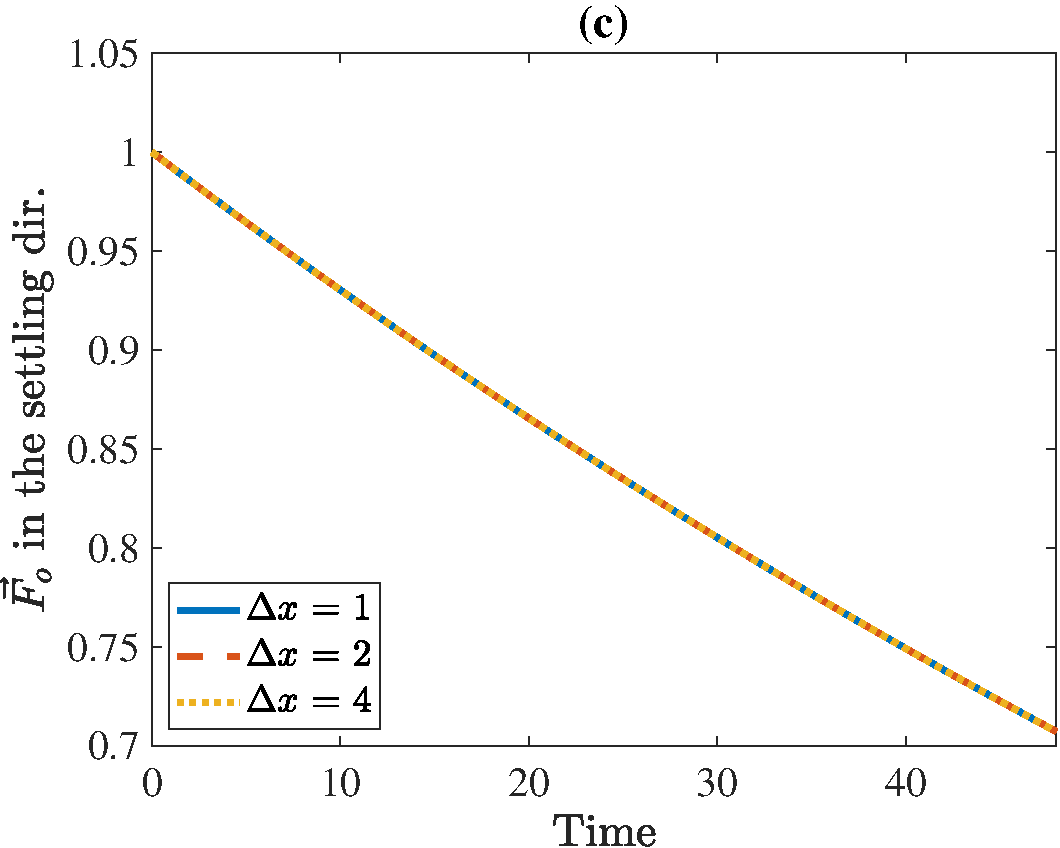
\includegraphics[scale=0.35]{./figures/fig_NC10_dx_Fo3_all}
		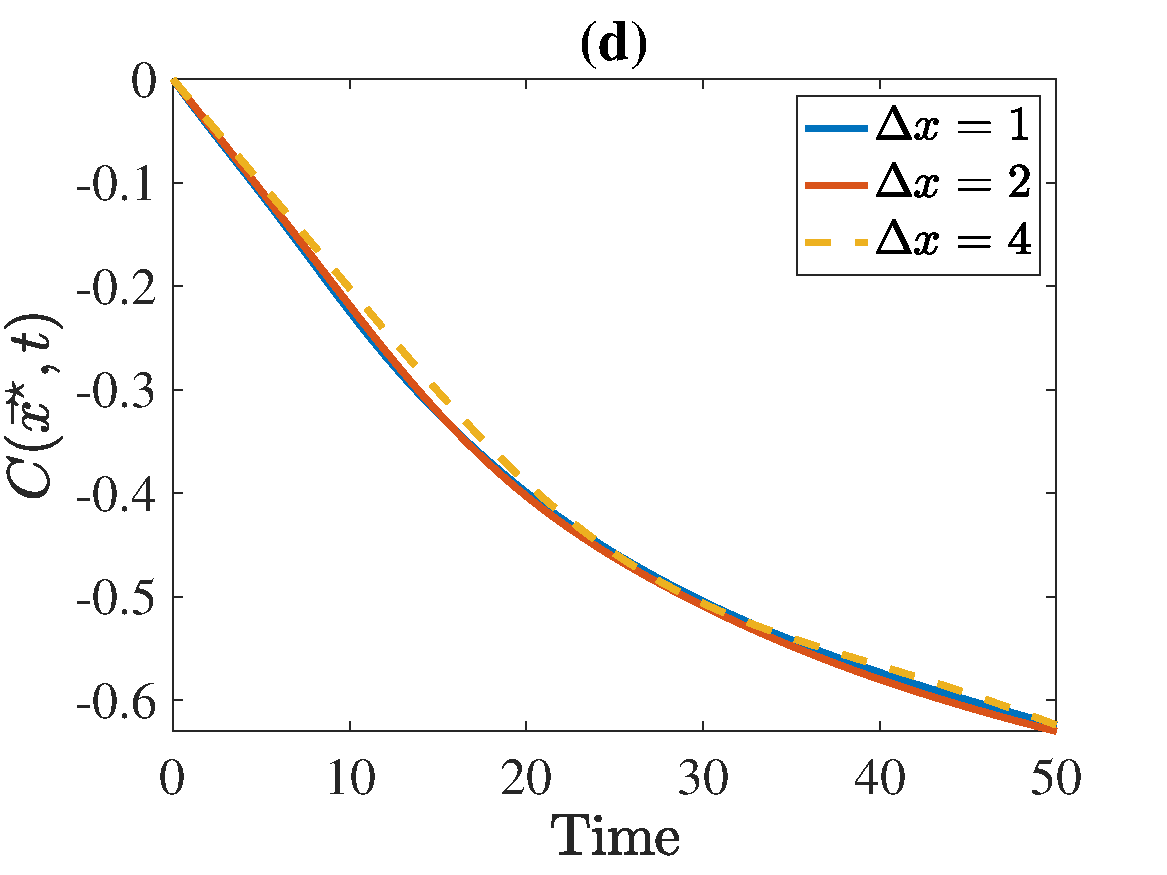
\includegraphics[scale=0.35]{./figures/fig_NC10_dx_C_star_interp3}
	\caption{Compare various $\Delta x = 1, \ 2, \ 4$ in the domain size factor $s = 5$ with $\Delta t = 0.75$. We show (a) the settling speed, (b) the position of the center of mass, (c) the vertical force on the aggregate, and (d)the value of the perturbation near the aggregate.}
	\label{fig_NC10_compare_dx}
\end{center}
\end{figure}
As we saw in the first two validations, we observe quite a good agreement between all values of aggregate behavior, velocity, moved location, and drag, in Figure~\ref{fig_NC10_compare_dx}. If we had computation time or memory capacity constraints, these results in plots (a), (b), and (c) support that we can still obtain qualitative results to analyze a settling aggregate. 
\par
For the last plot (d), since we have different grid spacings, we were not able to capture the perturbation at the $\vec{x}^{\star}$ exactly for $\Delta x = 2$ and 4 cases.  
We thus used MATLAB built-in function \verb+interp3+ to interpolate the $C$ value at location $\vec{x}^{\star}$. We particularly select the nearest-neighbor method, which finds the value at the nearest sample grid point. We find the interpolation results seem to be reliable, having a good match with previous results of $C$ with various domain and time step sizes. 

% As we plan to use approximately 10 times larger aggregate to show the results in section~\ref{sec:stratified_results}, it is inevitable to adjust both grid and time step sizes. 
\par
\vphantom{D}
\par
Before we close this section, we want to mention that it is difficult to say we obtained the "correct" since we do not have any analytic solutions. The validations we provide here are to exhibit convergence and estimate the size of the errors made due to time and space discretization and finite domain size effects.
The results we described in this section were confirmed with simulations of an aggregate made with 50 cubes, and similar trends were observed. We leave larger aggregate model simulations in the next section.
%-----RESULTS-----------------------------
\section{Simulation results}
\label{sec:stratified_results}
\subsection{Base case analysis}
Since there are a few parameters we are interested in varying, we decide on setting a base case to compare further simulations. To explore assorted shapes, we use 50 cubes to form an aggregate. We particularly use the aggregate shape in Figure~\ref{fig_NC50_base_seed2}. 
\begin{figure}[ht]
	\begin{center}
		\vspace*{3mm}
		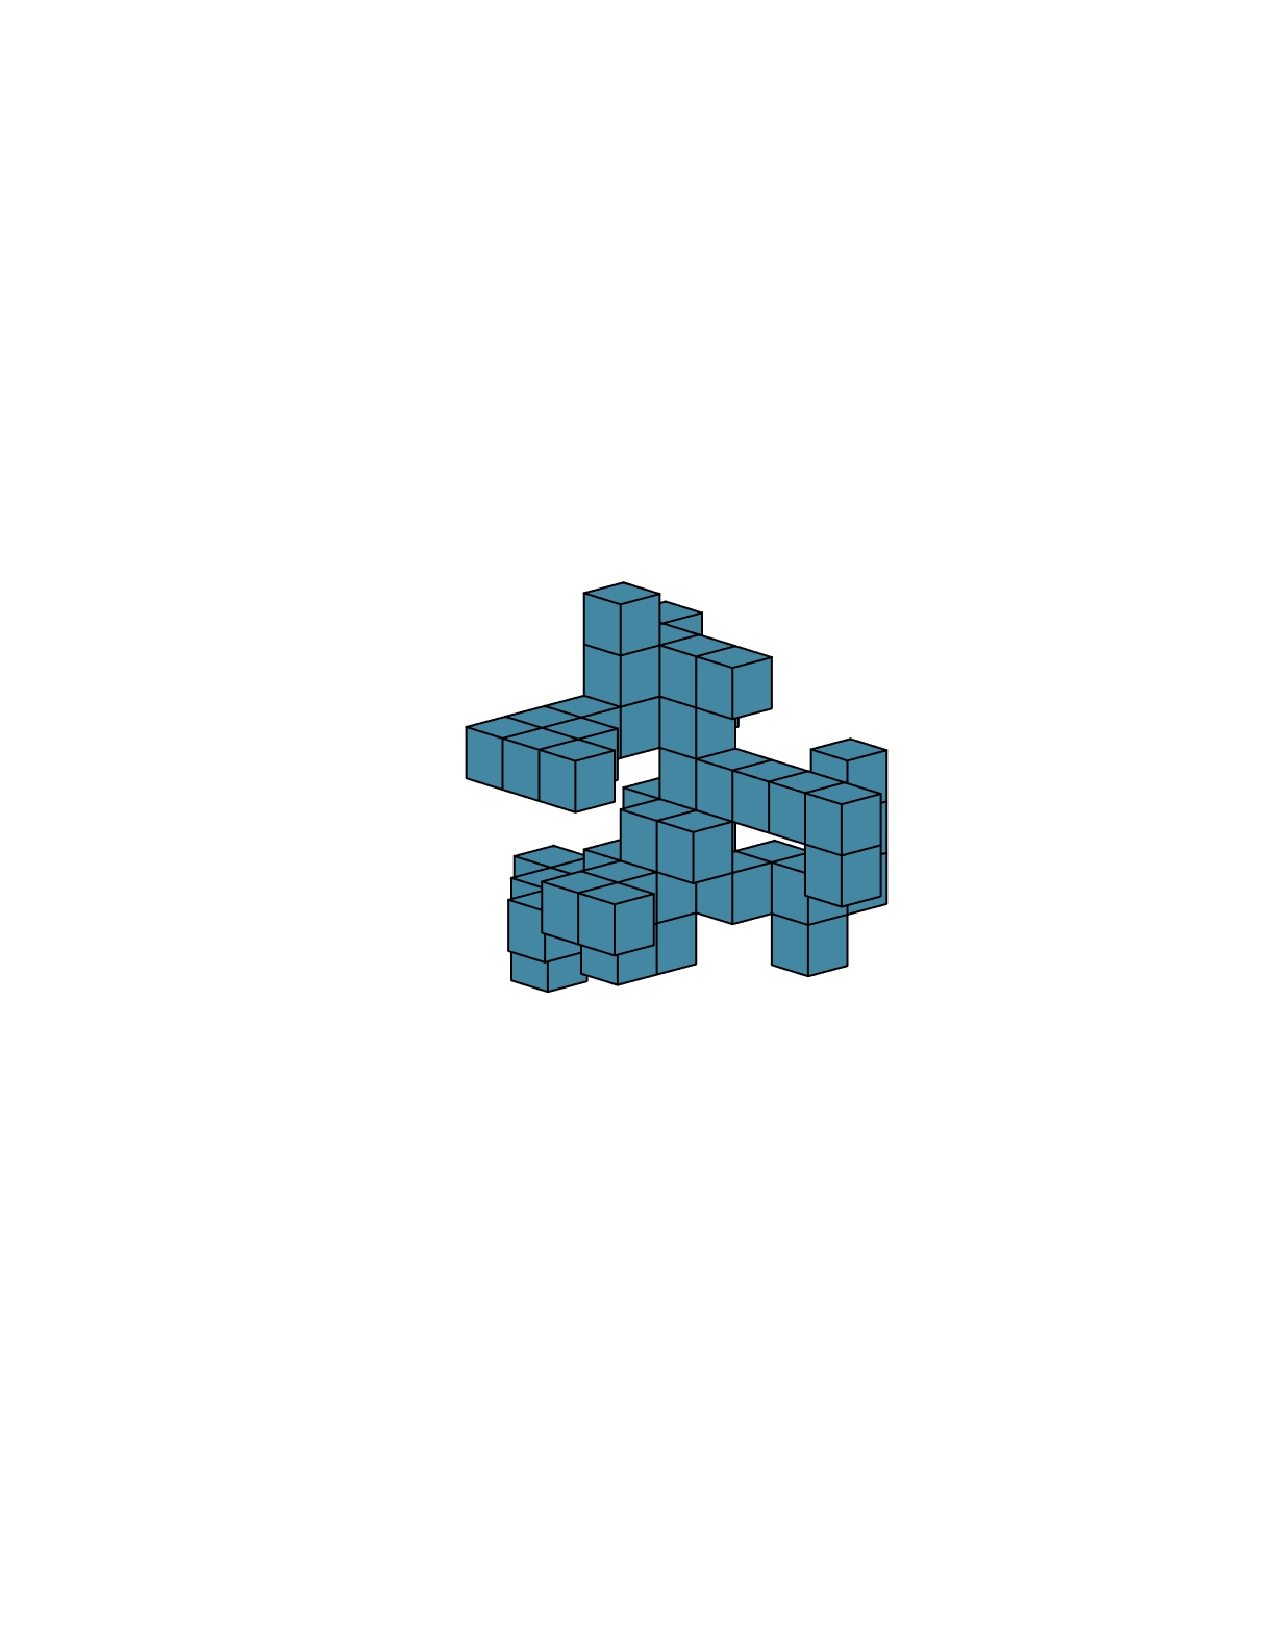
\includegraphics[scale=0.5]{./figures/fig_NC50_seed2}
	\caption{The base aggregate model (random seed number 2) with 50 cubes.}
	\label{fig_NC50_base_seed2}
\end{center}
\end{figure}
To avoid any stability issues while being computationally efficient, we choose the time step size $\Delta t = 0.5$ and grid spacing $\Delta x =1$. In section~\ref{sec:ch3_validation}, we have shown that these choices provide good accuracy. Moreover, we found that simulating the settling aggregate in the domain size with the scaling factor $s = 3$ is sufficient to have negligible boundary effects.  Also, we apply Pe = 100 as we did for the homogeneous model in Chapter~\ref{sec:ch2_CO2_simulation} for this base model.
\begin{figure}[ht]
	\begin{center}
		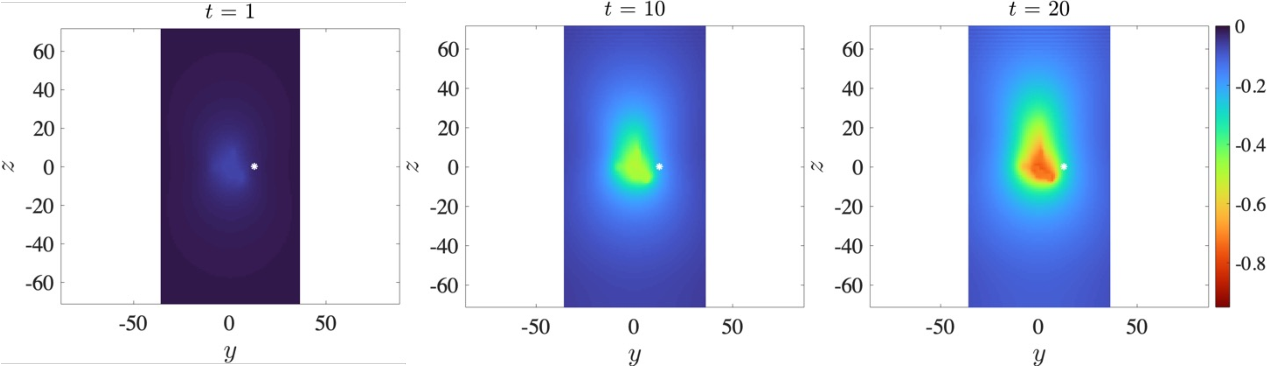
\includegraphics[scale=0.65]{./figures/fig_NC50_snaps_pt1.pdf}
		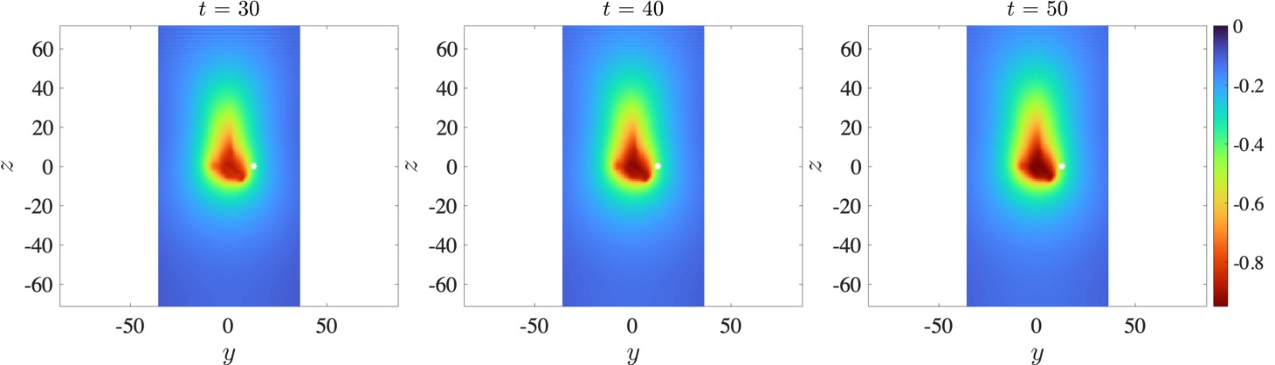
\includegraphics[scale=0.65]{./figures/fig_NC50_snaps_pt2.pdf}
	\caption{Concentration dynamics with the base model case at various times.}
	\label{fig_NC50_snaps_all}
\end{center}
\end{figure}
\par
Additionally, we select the stratification strength $\gamma$ more systematically. 
To do so, we first consider the travel distance of an aggregate, denoting it as $z_T$. In Figure~\ref{fig_sample_agg10}, we showed that the aggregate is initially located in the middle of the domain. We are interested in observing a setup where $\gamma$ is as large as possible while allowing the aggregate to travel about $z_T = 6R_a$, before
reaching its level of neutral buoyancy.
% an aggregate with its radius $R_a$ settles approximately half of the fluid domain, which is $2 s R_a$. It implies that we set $z_T = 2sR_a$.
At the vertical level $z_T$, equation (\ref{eq_rho_bg}) tells us to have background fluid density 
\begin{equation}
	\rho_{bg} = \rho_0 (1-\gamma z_T) =	\rho_0 (1 - 6R_a \gamma).
	\label{eq_compute_G}
\end{equation}
Meanwhile, we want the aggregate density $\rho_a$, which is defined in equation (\ref{eq_rho_a}), to reach neutral buoyancy. To see this, we assume the initial aggregate density, when its fluid portion $\rho_f$ is $\rho_0$, is equal to the background fluid density after stop settling, i.e., $\rho_a = \rho_{bg}$. 
For an aggregate composed of 50 cubes, we have an estimated average radius $R_a \approx 9$~\cite{yoo_hydrodynamic_2020}, and thus we find $\gamma \approx 4 \times 10^{-4}$.  
\begin{figure}[h]
	\begin{center}
		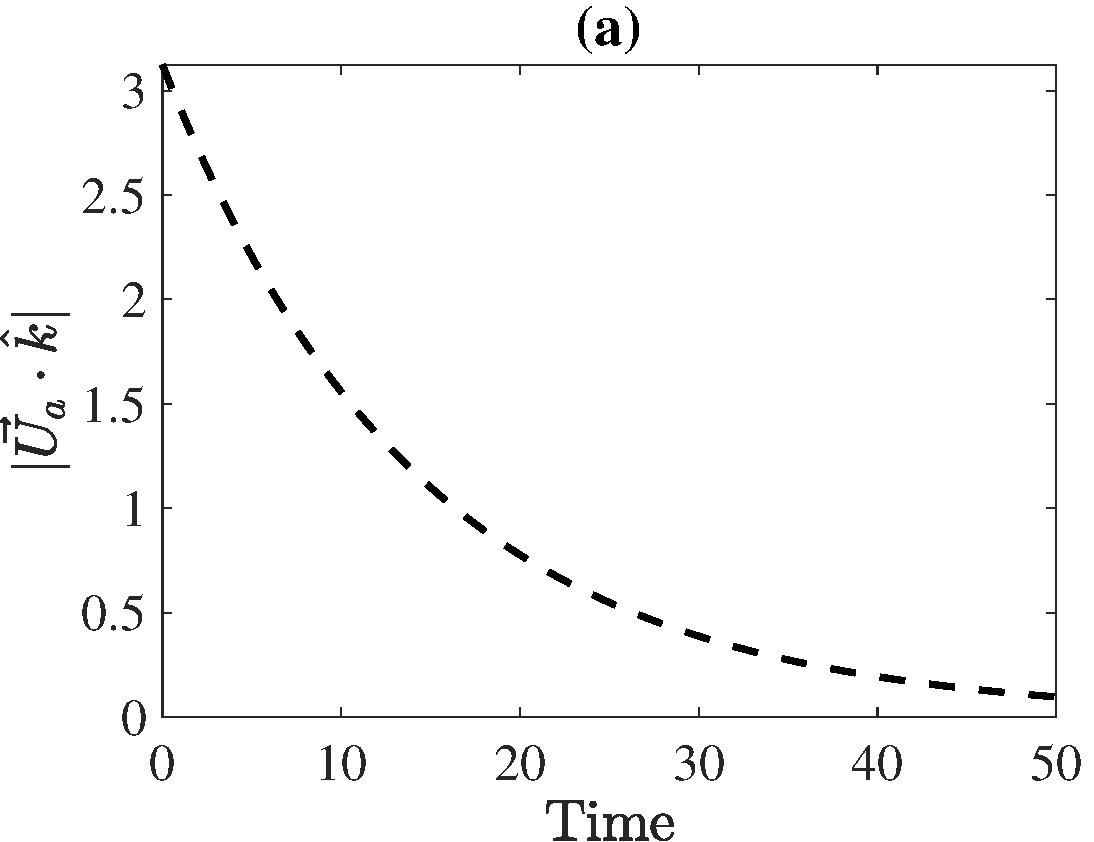
\includegraphics[scale=0.35]{./figures/fig_NC50_bs_Ua3_all.pdf}
		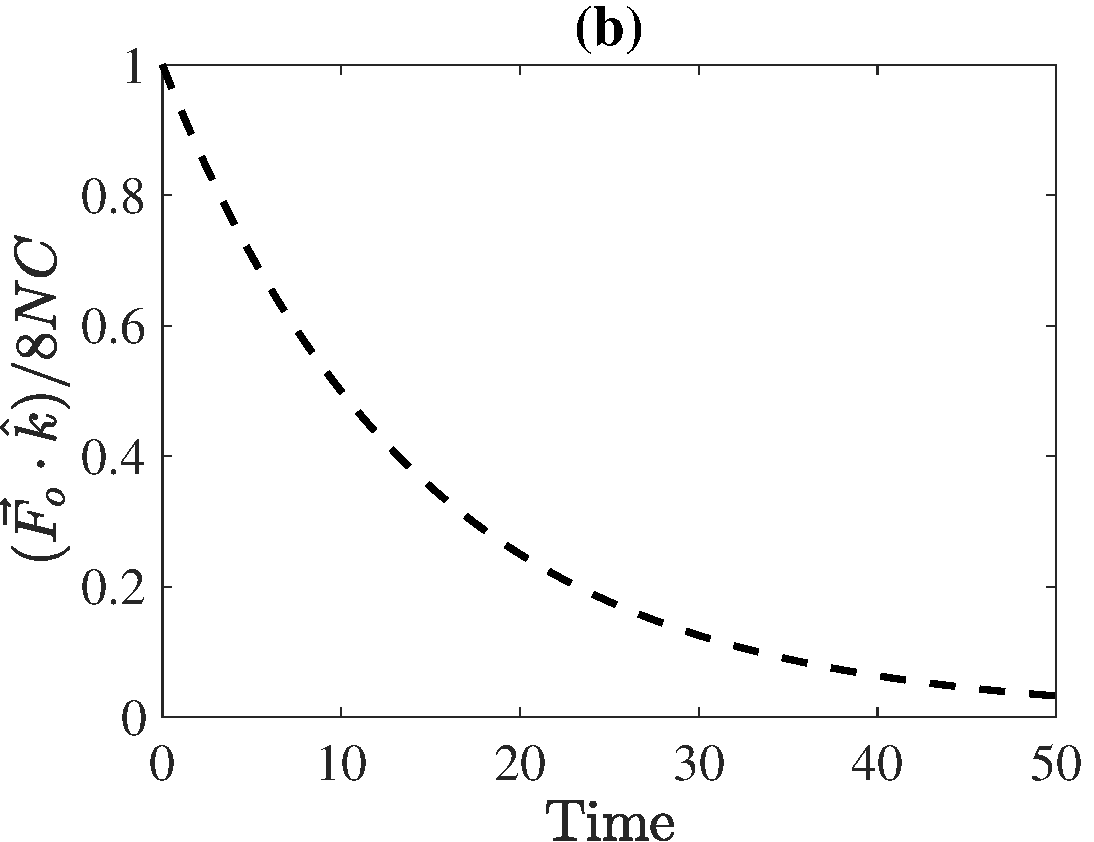
\includegraphics[scale=0.35]{./figures/fig_NC50_bs_Fo3_all}
		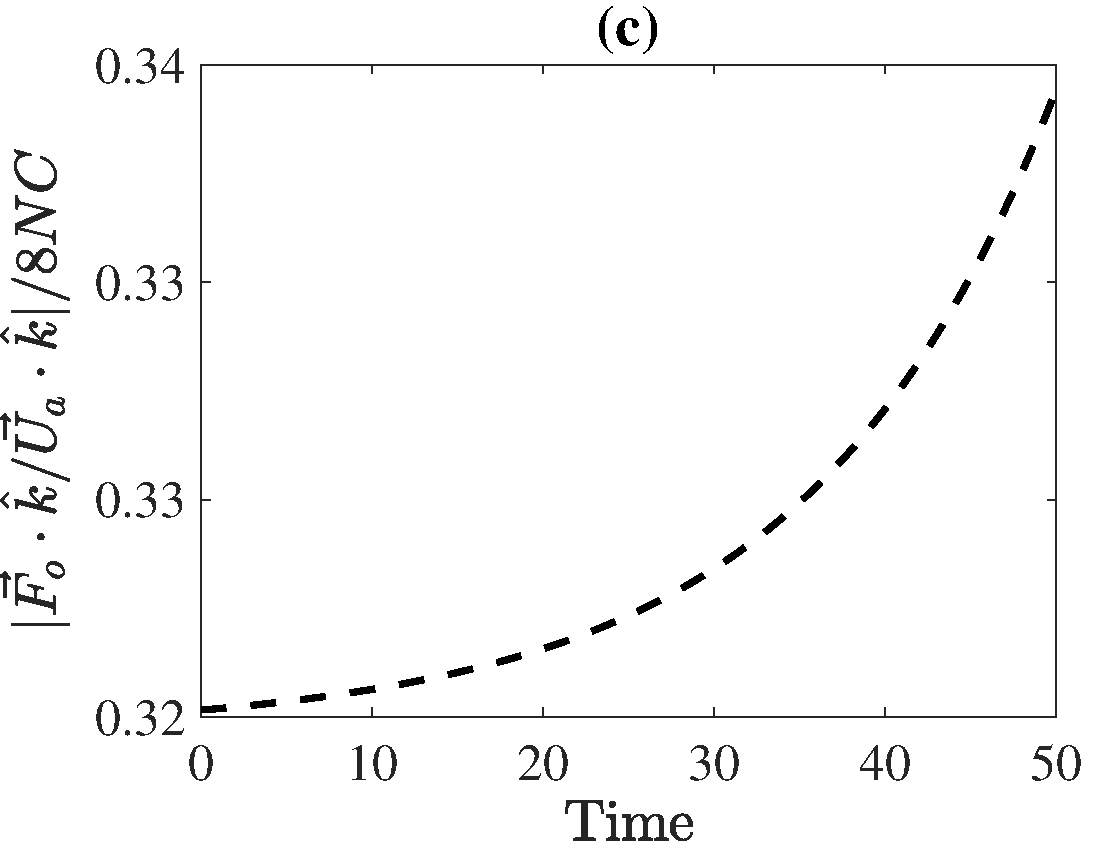
\includegraphics[scale=0.35]{./figures/fig_NC50_bs_Fo3Ua_ratio}
		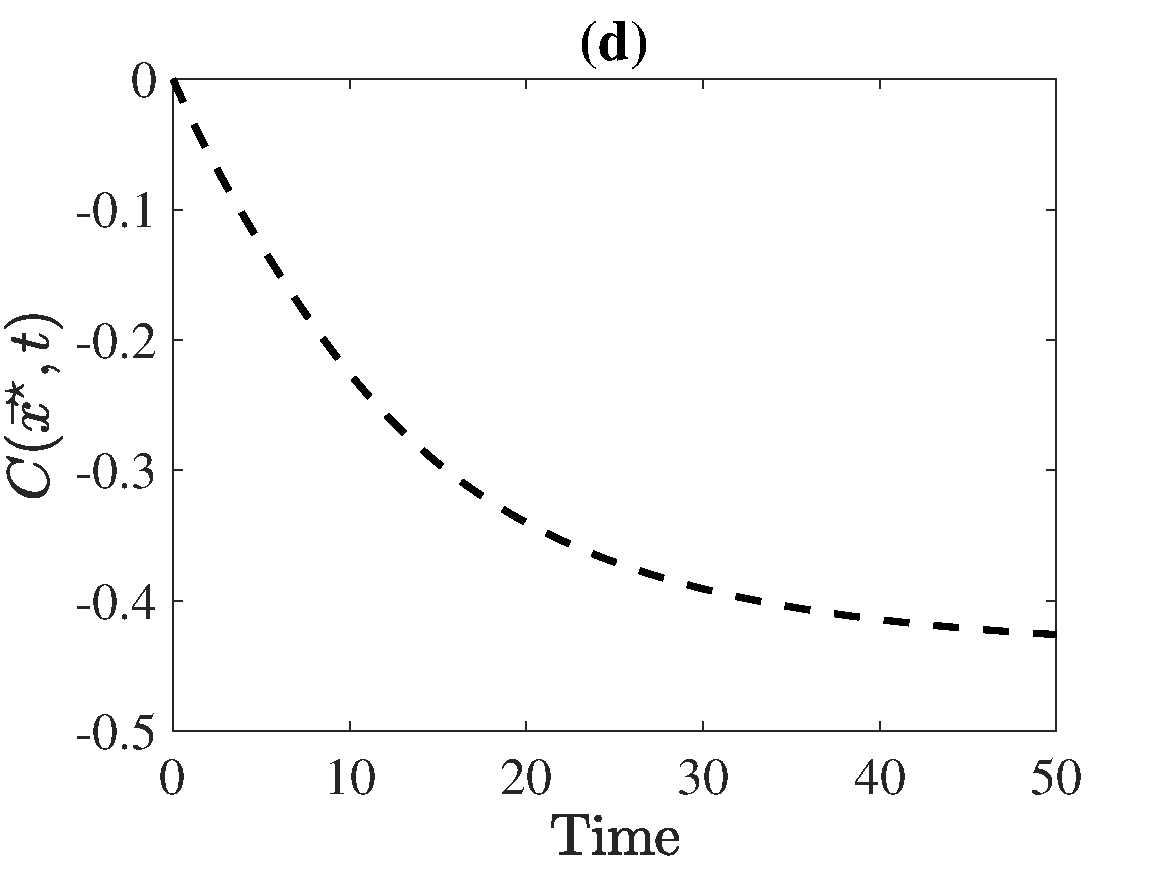
\includegraphics[scale=0.35]{./figures/fig_NC50_bs_C_star}
	\caption{Compare various Péclet numbers. We show (a) the settling speed, (b) the vertical component of normalized drag force on the aggregate, (c) the ratio of (b) to (a) values, and (d) the perturbation at position $\vec{x}^{\star}$. }
	\label{fig_NC50_base_case_all}
\end{center}
\end{figure}
\par 
In Figure~\ref{fig_NC50_snaps_all}, we show several 2D snapshots, sliced in the middle of the domain ($x = -0.74$), of perturbation $C$ at various times. Note that we see negative values of $C$ since the perturbation is a concentration difference from its initial one. 
We can observe much higher perturbation around the aggregate that increases in magnitude as time goes on, as the aggregate entrains upper-level concentration. 
\par
We observe the aggregate behavior more closely in Figure~\ref{fig_NC50_base_case_all}. As we introduced in the previous chapter, we measure (a) the settling speed and (b) the normalized total drag of the aggregate. We also exhibit the ratio of total drag to the settling speed in plot (c) as a measure of the coefficient in the linear relationship between drag and velocity
that is observed in Stokes flow. Although both settling speed and drag seem to be decreasing over time, as fluid buoyancy balances, we find that their ratio (c) increases non-linearly. This implies that the stratification of the fluid plays a role in the aggregate's settling behavior, not only by reducing the buoyancy but also through the entrained fluid. 
We would have observed a horizontal line if the surrounding fluid does not affect aggregate motion as it settles in a homogeneous fluid. 
\par
In the last plot (d), we observe the perturbation at a particular location outside the aggregate boundary. It is the white star point $\vec{x}^{\star} = (-0.74, 12.74, 0.24)$ in Figure~\ref{fig_NC50_snaps_all}. This point is approximately (1.01 + $R_m$) away from the center of mass of the aggregate. The perturbation is expected to grow in magnitude over time. As the settling motion slows down, the magnitude of perturbation also smoothes out. 
\par
In the next section, we explore various shapes of aggregates made with 50 cubes, in addition to the base case. Afterward, we will observe the effects of varying Péclet numbers and background fluid density stratification. 
\begin{figure}[ht]
	\begin{center}
		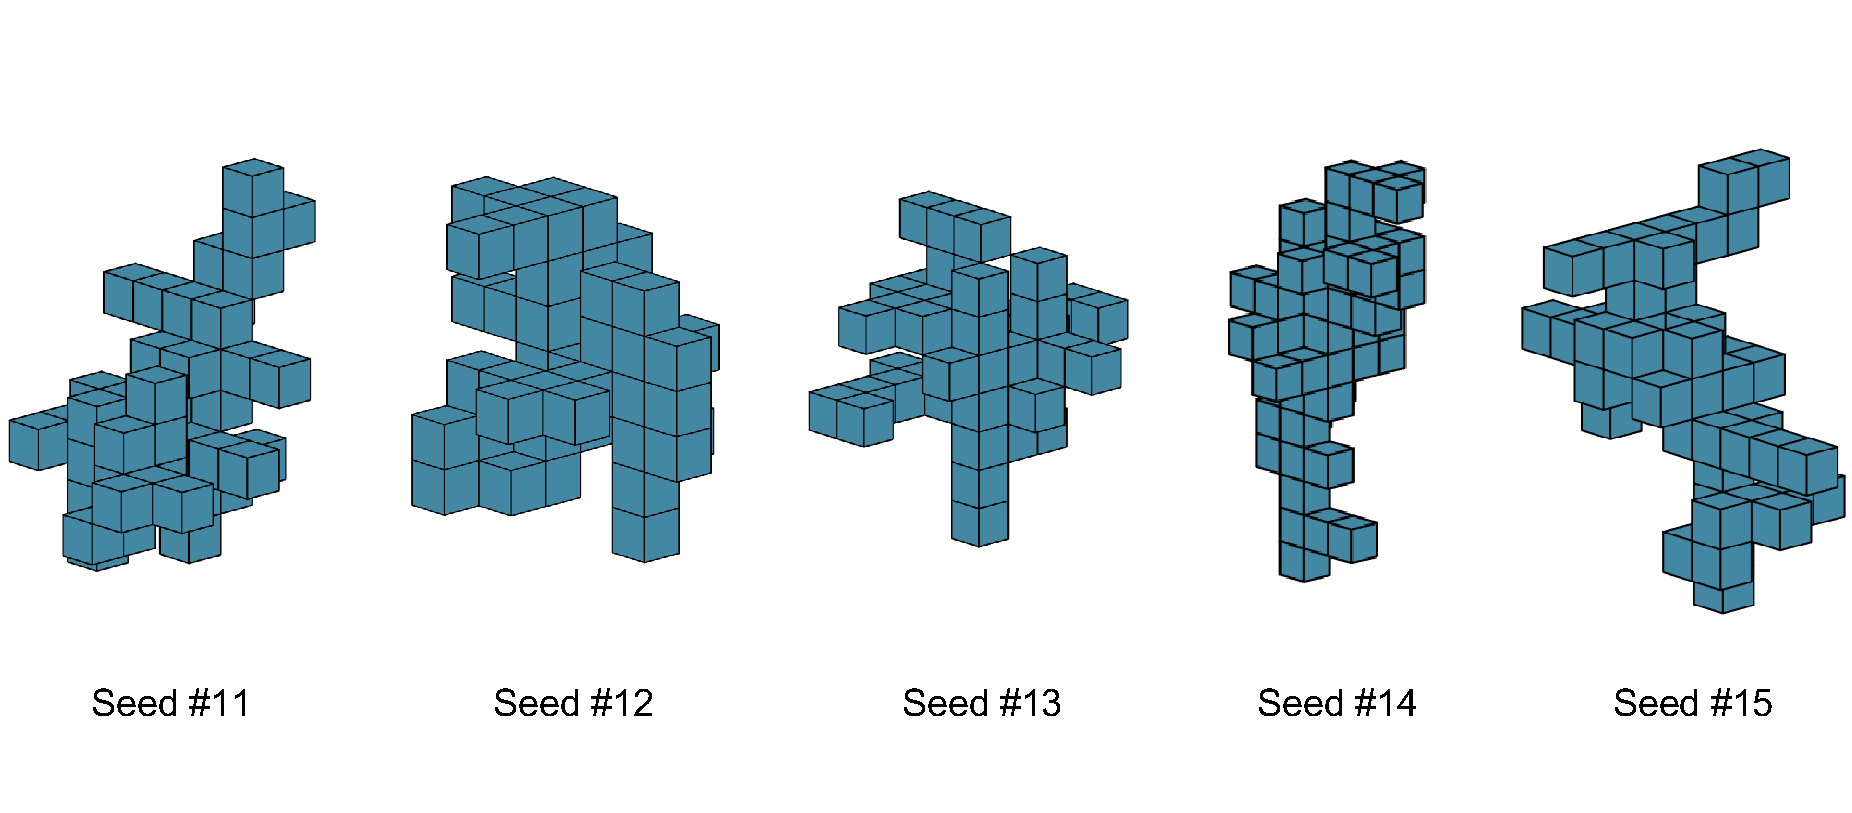
\includegraphics[scale=0.45]{./figures/fig_seed11_15_all.pdf}
	\caption{Five sample aggregates composed of 50 cubes.}
	\label{fig_seed11_15_all}
\end{center}
\end{figure}
\par
\subsection{Various shapes of aggregates}
We first run simulations with randomly shaped aggregates using 50 cubes, in addition to the base case model that is the random seed \#2. We create five more different aggregates, numbering seeds from \#11 to \#15. See Figure~\ref{fig_seed11_15_all}.
With these six sample aggregates, we examine their behaviors, as shown in Figure~\ref{fig_NC50_Seeds}.
\begin{figure}[ht]
	\begin{center}
		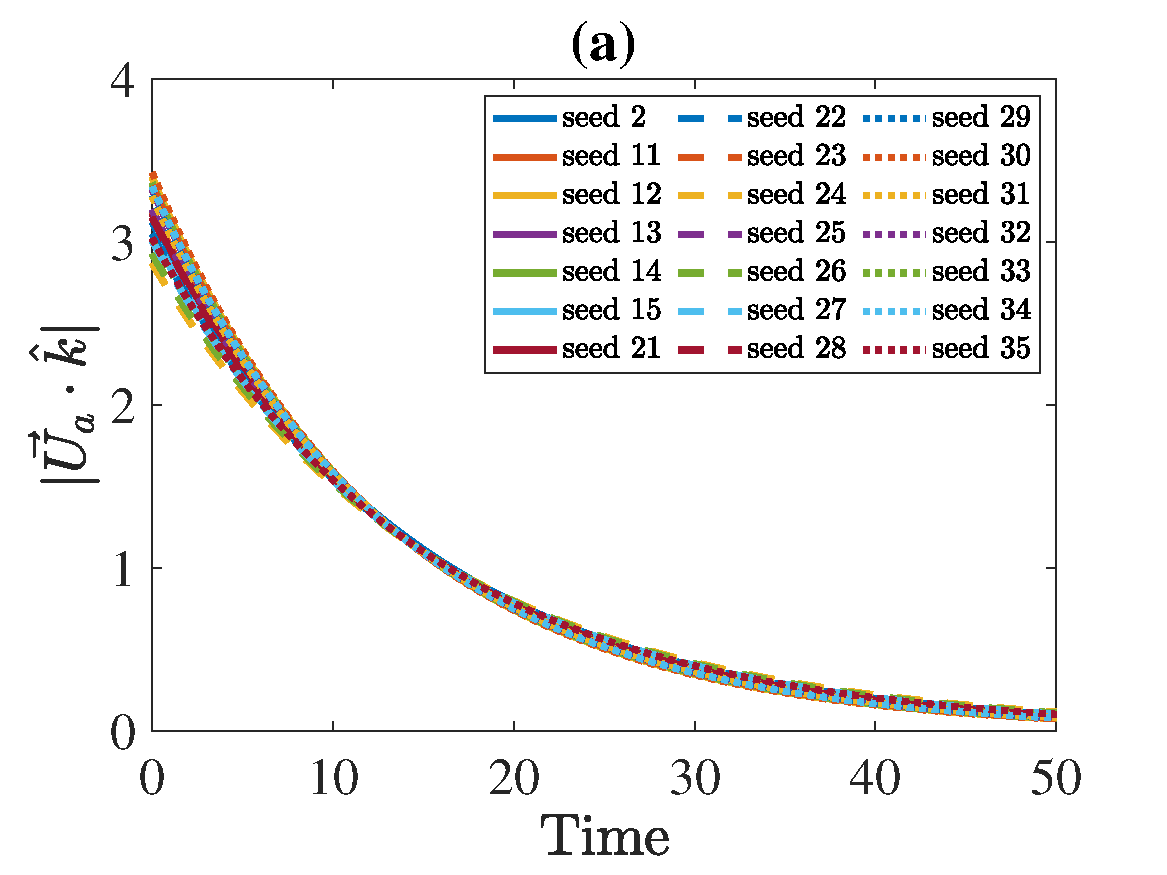
\includegraphics[scale=0.29]{./figures/fig_NC50_sd_Ua3_all}
		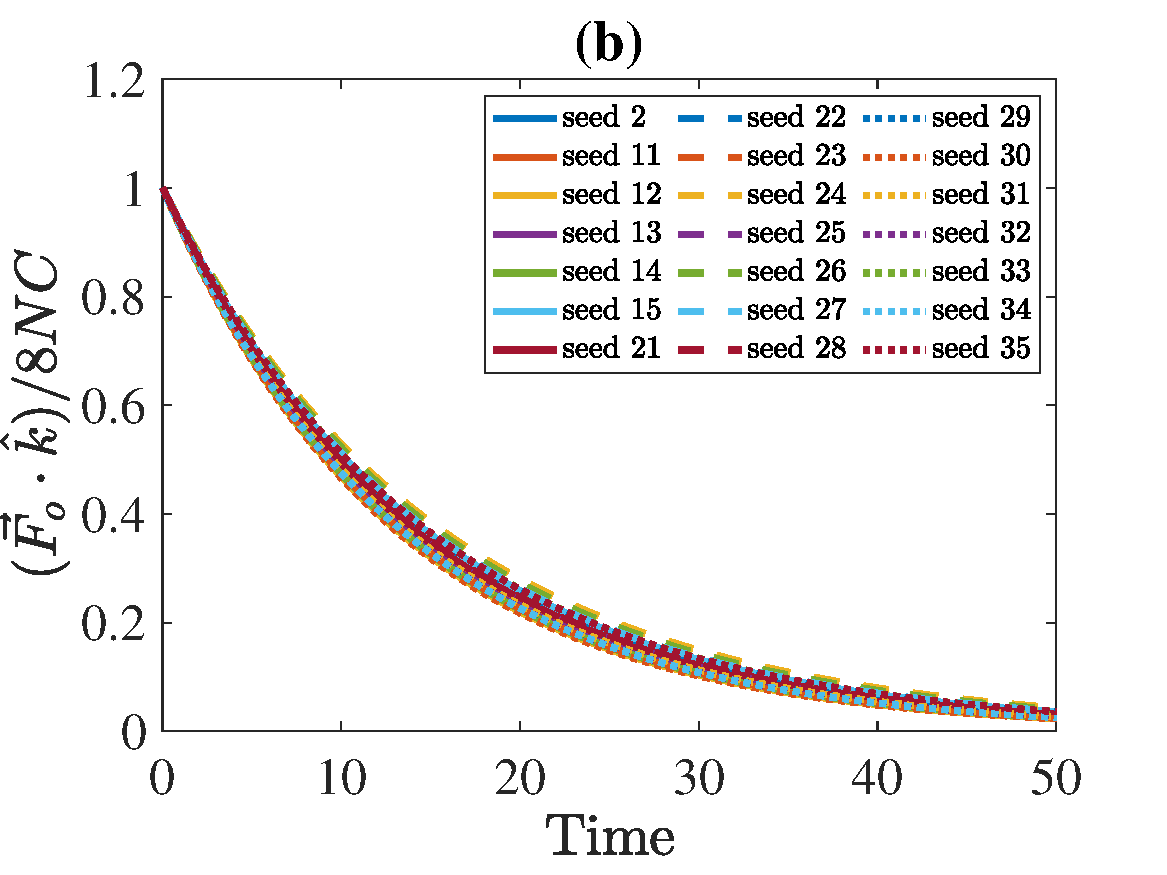
\includegraphics[scale=0.29]{./figures/fig_NC50_sd_Fo3_all}
		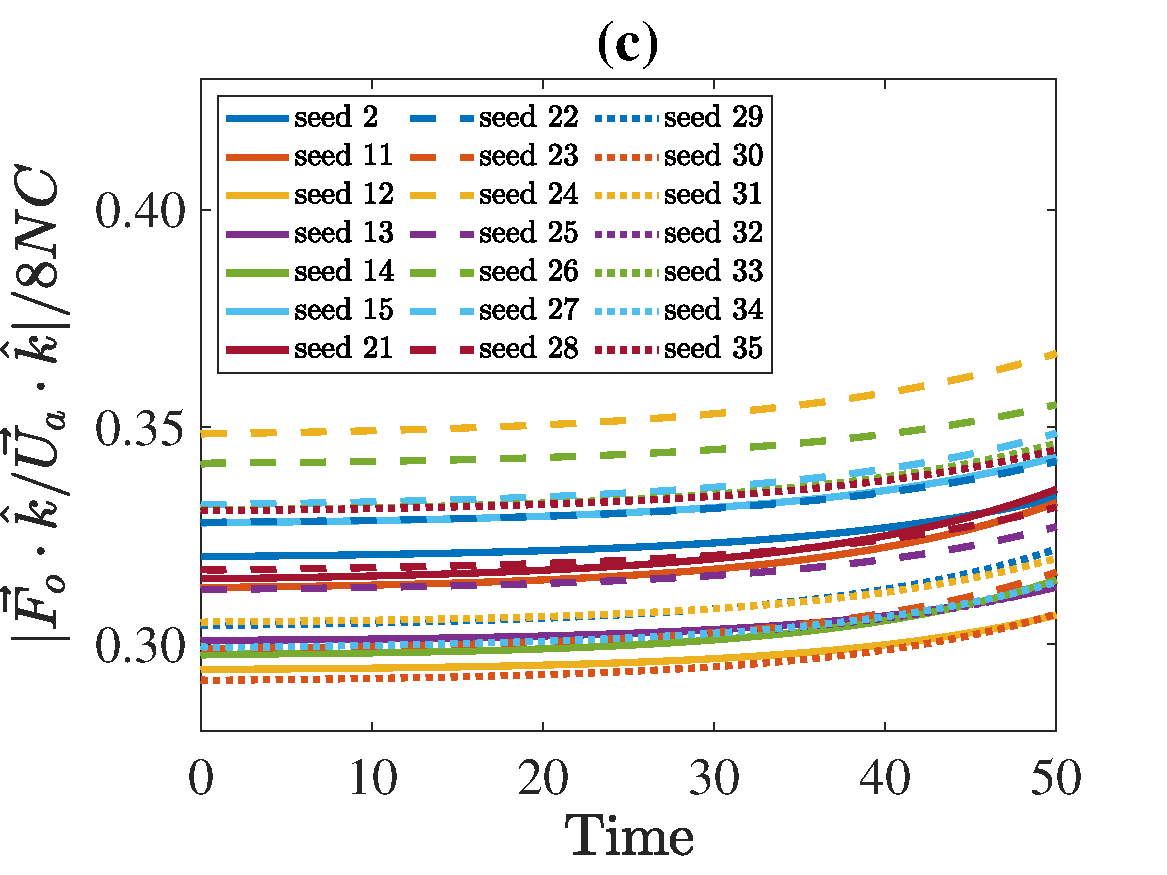
\includegraphics[scale=0.29]{./figures/fig_NC50_sd_Fo3Ua_ratio}
		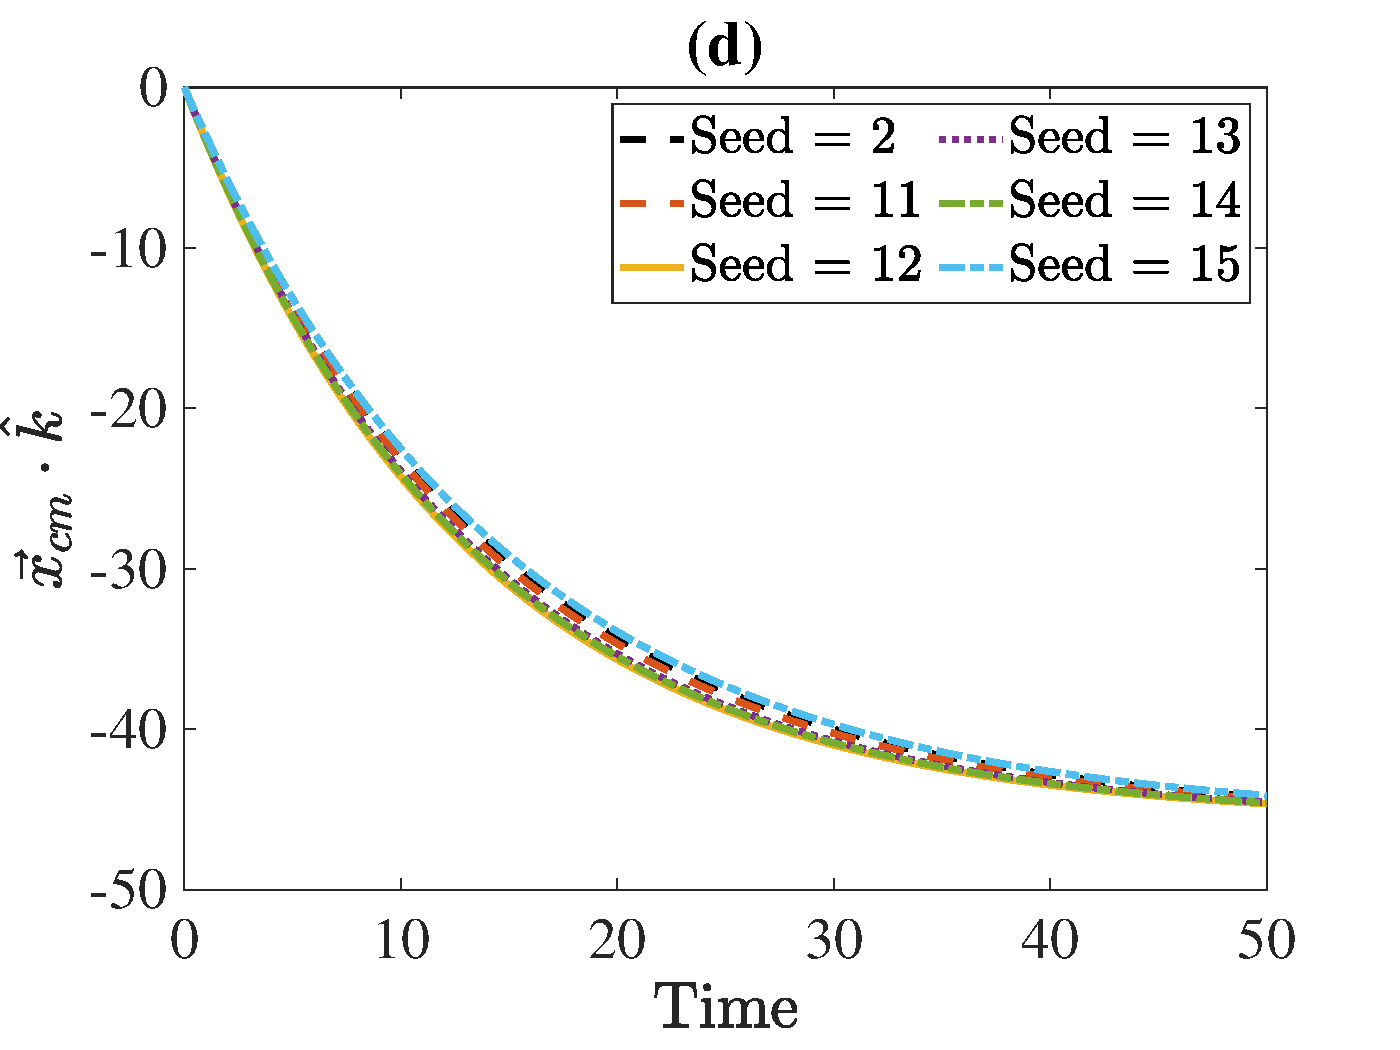
\includegraphics[scale=0.29]{./figures/fig_NC50_sd_cm3_all}
	\caption{Compare various shapes of aggregates made with 50 cubes. We show their (a) settling speed, (b) drag force on the aggregate in the settling direction, (c) ratio of (b) to (a) values, and (d) position of the center of mass.}
	\label{fig_NC50_Seeds}
\end{center}
\end{figure}
\par
% When we analyzed the drag forces in a homogeneous fluid in Chapter~\ref{sec:results_translationflow}, we observed the drag distribution of about 15\% with aggregates made with 50 cubes; see Figure~\ref{fig_drag_raw}.
There are some variations (less than 16\%) in aggregates settling behaviors, yet their speed, drag, and $\vec{x}_{cm}$ locations seem to have overall similar motions. 
Meanwhile, plot (c) shows larger differences between each aggregate shape. 
We find this interesting feature that the drag-velocity ratio spread shows approximately a 12\% difference range and 5\% away from their mean value(at the final time). 
Note that the sample mean value at the final time $t = 50$ is about 0.3241.
This demonstrates that modeling an aggregate as a sphere cannot accurately capture all physical forces involved.
\par
Based on this mean value of six samples, we can estimate the number of random seeds, $N_{sd}$, we should simulate to obtain a finer result. In particular, we want to get the $N_{sd}$ such that the relative error between the standard error ($SE$) and standard error of the mean ($SEM$) is 1\%, i.e.,
\begin{equation}
	\frac{|SE \ - \ SEM|}{SE} < 1 (\%).	
\end{equation}

In our case, we have
\begin{equation}
	SE \ = \frac{\text{Standard deviation with all  } N_{sd}}{\sqrt{N_{sd}}}
\end{equation}
and
\begin{equation}
	SEM \ = \frac{\text{Standard deviation of 6 samples}}{\sqrt{6}}.
\end{equation}
However, since we do not know the numerator of $SE$, we assume that it is the same as the sample standard deviation. We then can solve for $N_{sd} \geq 37$. Once time allows, we plan to run simulations with $N_{sd}$ many different randomly formed aggregates. 

\subsection{Various Péclet number, Pe}
Next, we vary Péclet numbers; Pe $=1$ and $ 10$ comparing the simulations to the base case for which Pe = 100.  As a smaller Péclet number 
implies more diffusive effects under the same advection rate, we look for differences in perturbation, while we predict to observe almost identical aggregate dynamics (velocity, traveling location, and total drag). 
Since we have more numerical instability for lower Péclet numbers, we exceptionally reduce the time step size to $\Delta t = 0.1$ for all three Péclet number cases.
\begin{figure}[ht]
	\begin{center}
		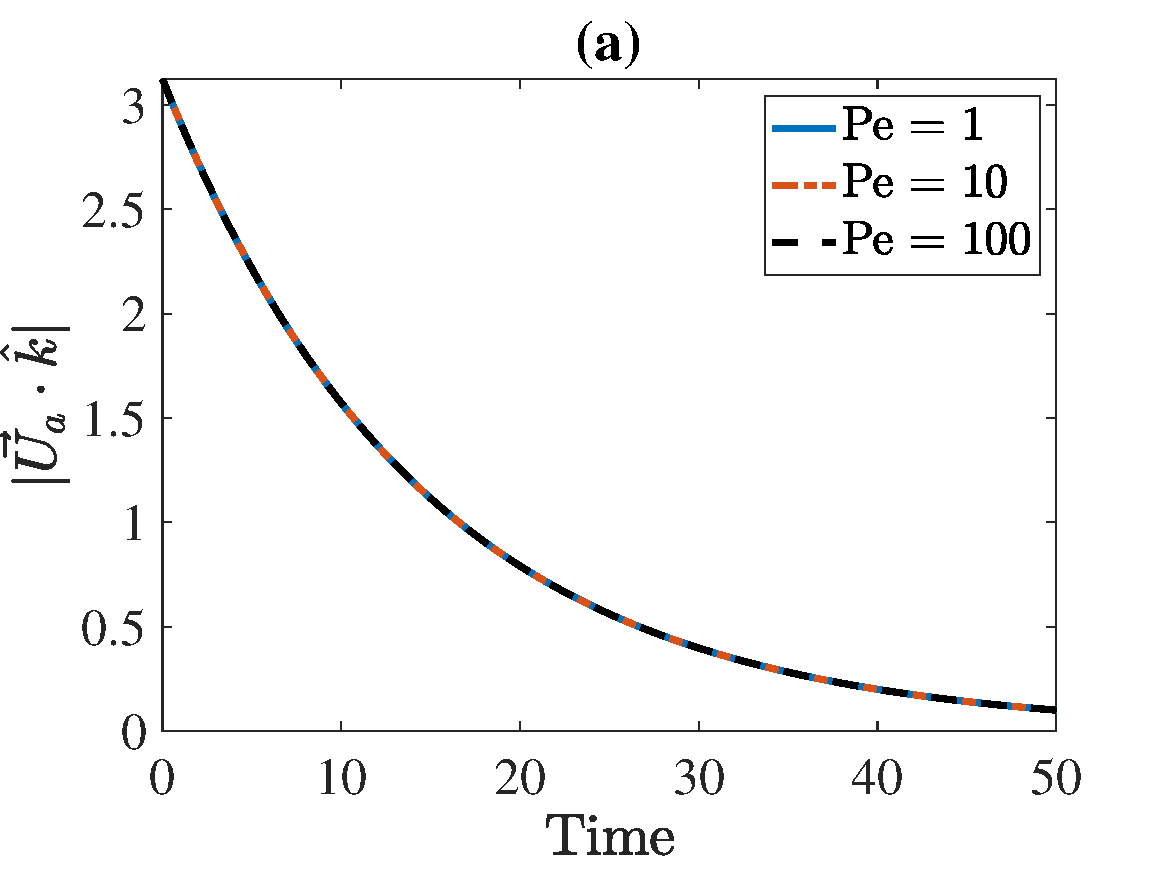
\includegraphics[scale=0.35]{./figures/fig_NC50_Pe_Ua3_all}
		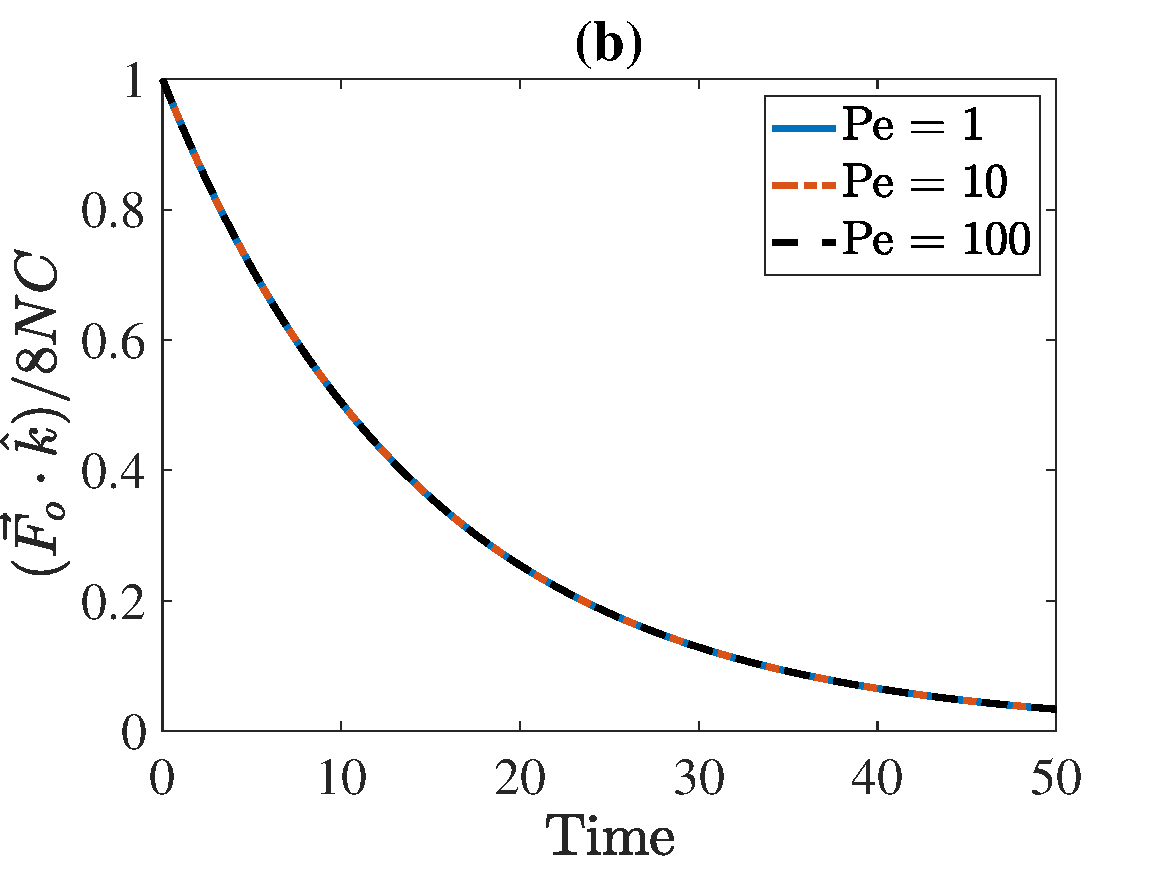
\includegraphics[scale=0.35]{./figures/fig_NC50_Pe_Fo3_all}
		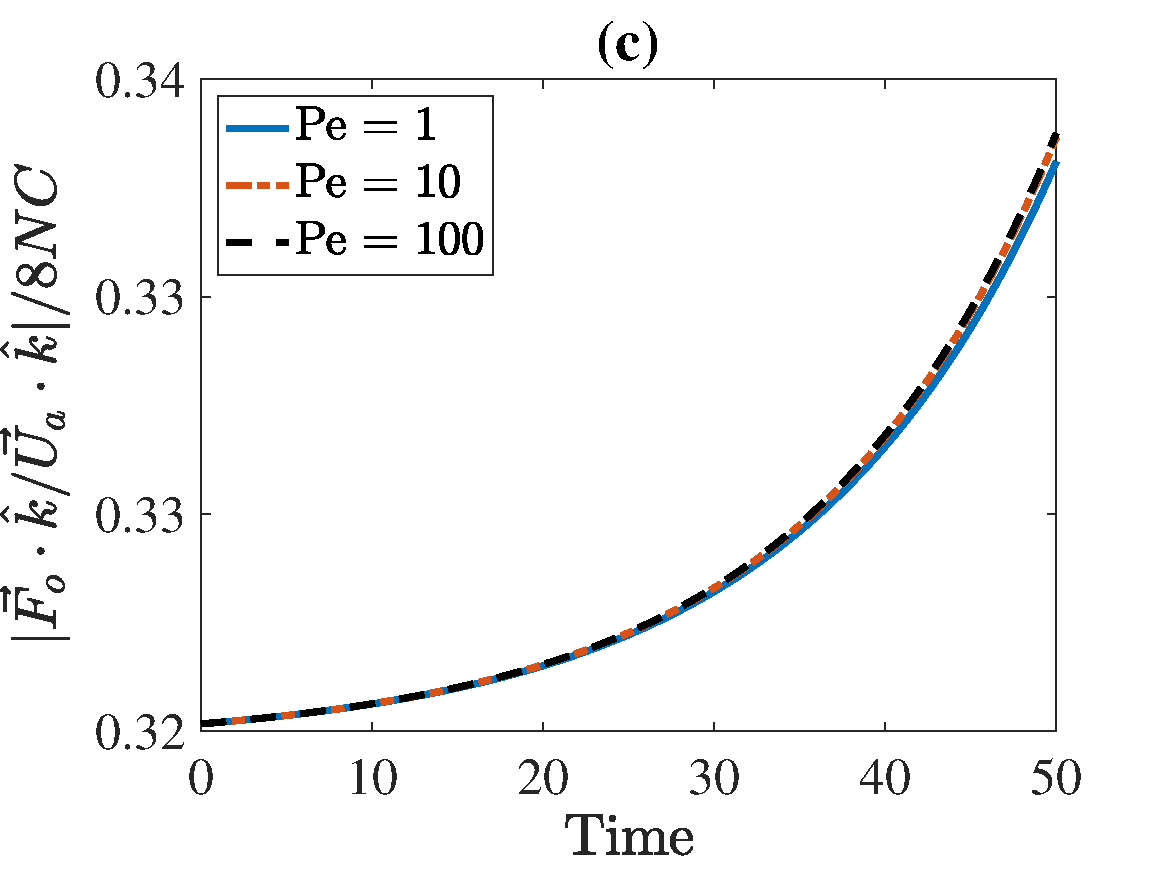
\includegraphics[scale=0.35]{./figures/fig_NC50_Pe_Fo3Ua_ratio}
		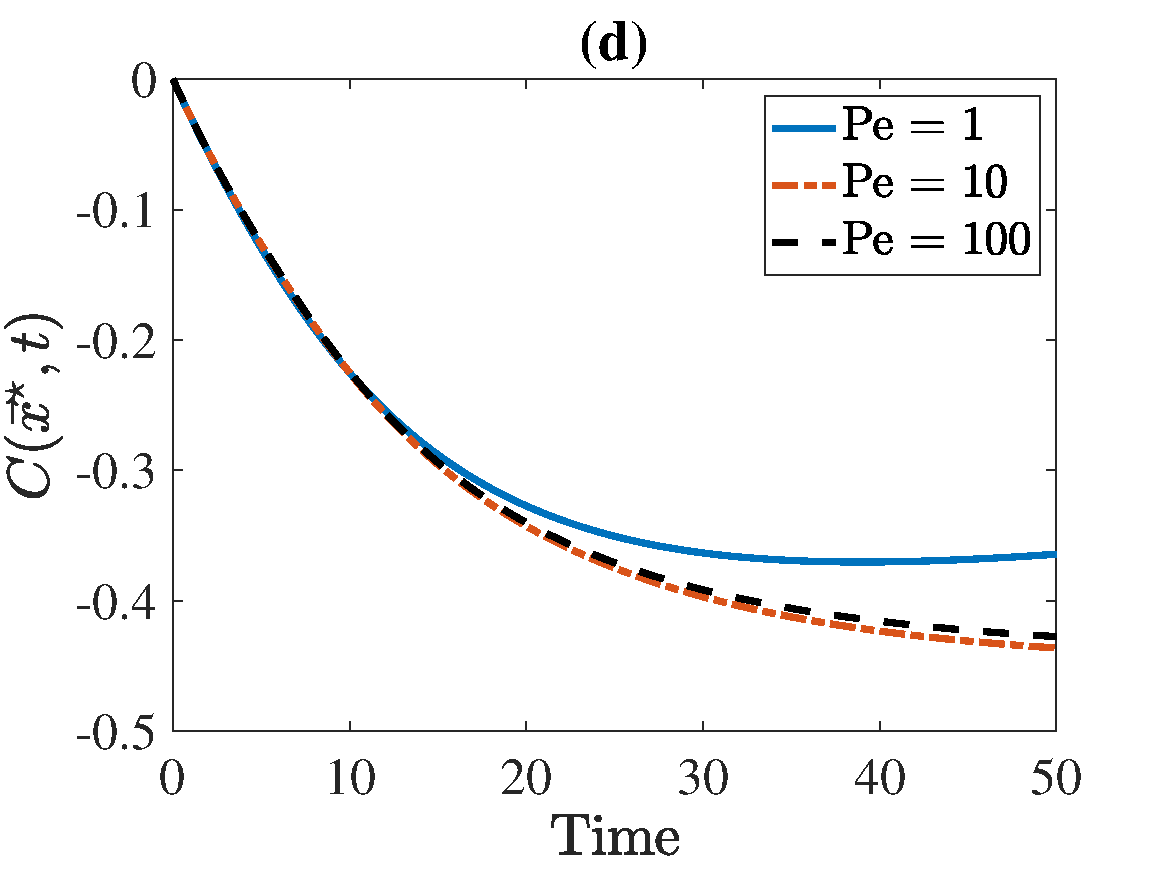
\includegraphics[scale=0.35]{./figures/fig_NC50_Pe_C_star}
	\caption{Compare various Péclet numbers. We show (a) the settling speed, (b) the vertical force on the aggregate, (c) the ratio of (b) to (a) values, and (d) the value of the perturbation near the aggregate.}
	\label{fig_NC50_Pe}
\end{center}
\end{figure}
\par
Figure~\ref{fig_NC50_Pe} shows no drastic variations between all three Péclet numbers, especially for the velocity and total drag. 
Focusing on the perturbation plot (d), we can see that more diffusion occurs for the smallest Péclet, Pe = 1, having steady perturbation after time $t = 30$.
Overall, it is clear that all four plots agree well with our expectations, even though the impact of varying the Péclet number is small in this regime. 
\subsection{Various stratification strength via $\gamma$}
Lastly, we investigate three different stratification strengths, $\gamma = 10^{-4} \times \left[ \ 1, \ 4 \ \text{(base case)}, \  6 \right]$. We anticipate observing conspicuous variations in both aggregate and fluid dynamics as we change the $\gamma$ value. Note that every other parameter is the same as the base case. 
\begin{figure}[h]
	\begin{center}
		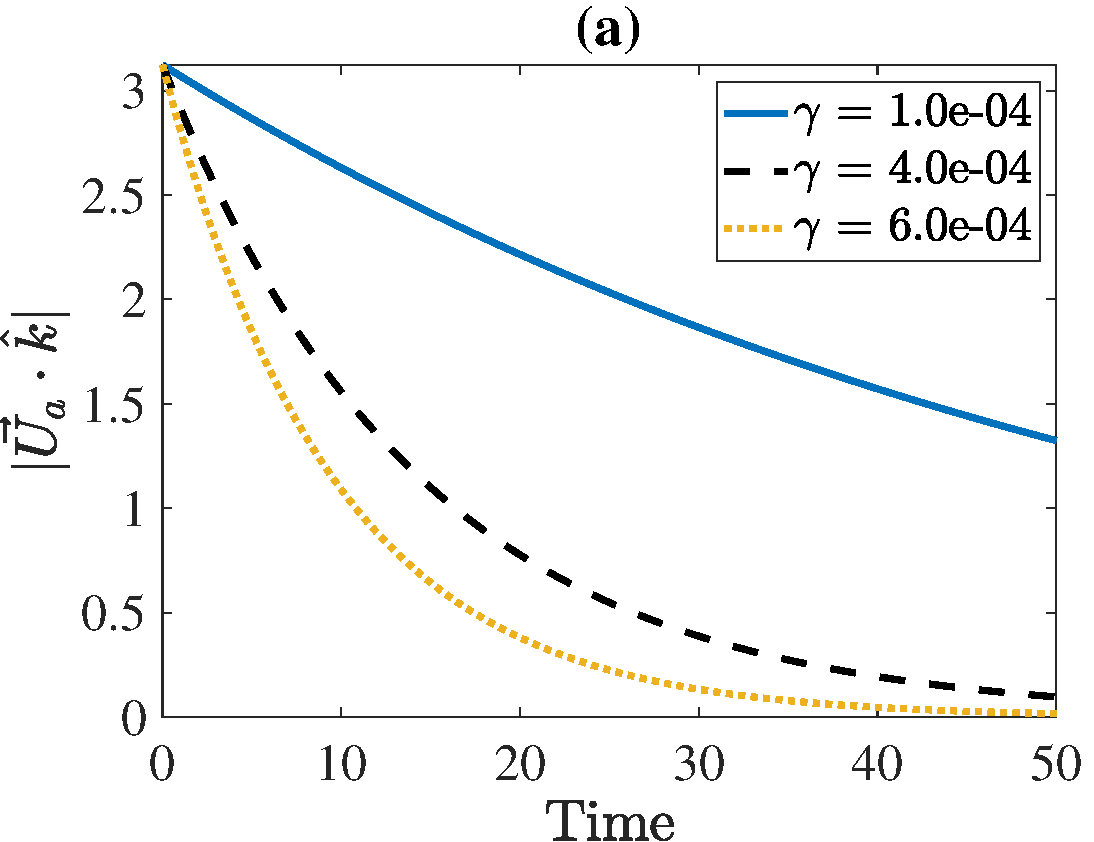
\includegraphics[scale=0.35]{./figures/fig_NC50_g_Ua3_all}
		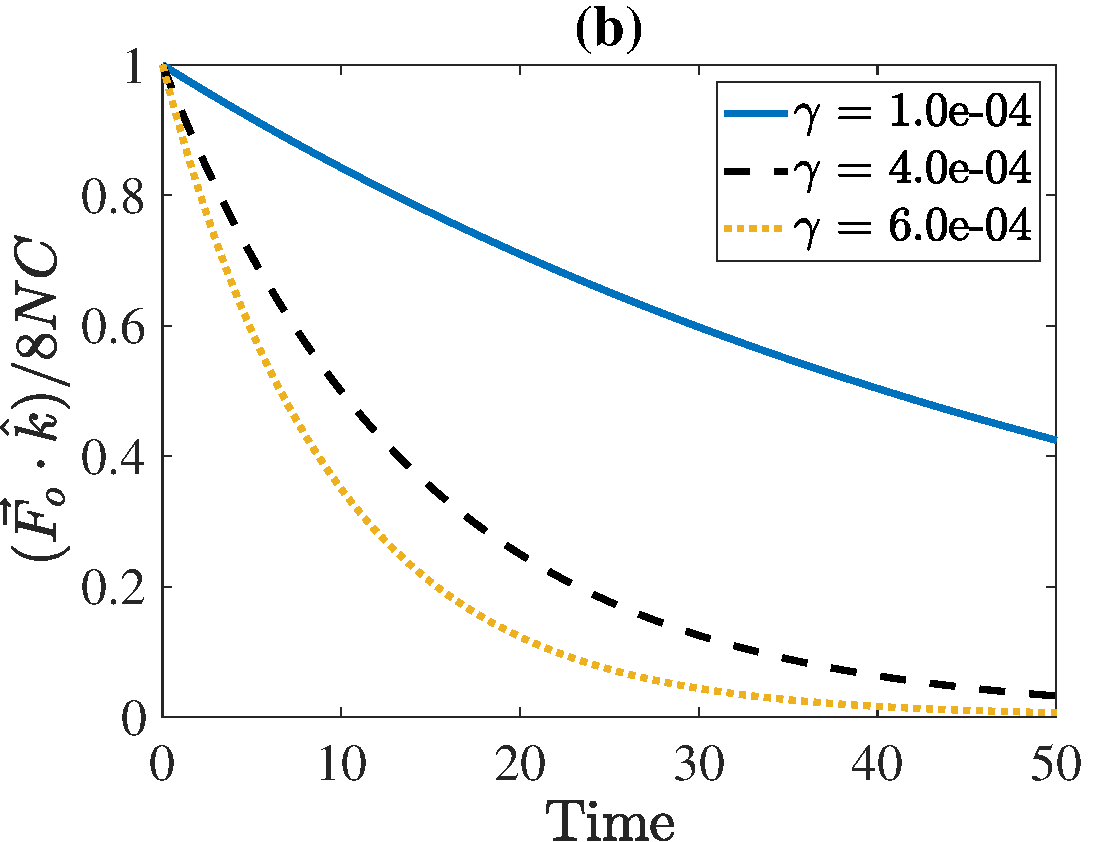
\includegraphics[scale=0.35]{./figures/fig_NC50_g_Fo3_all}
		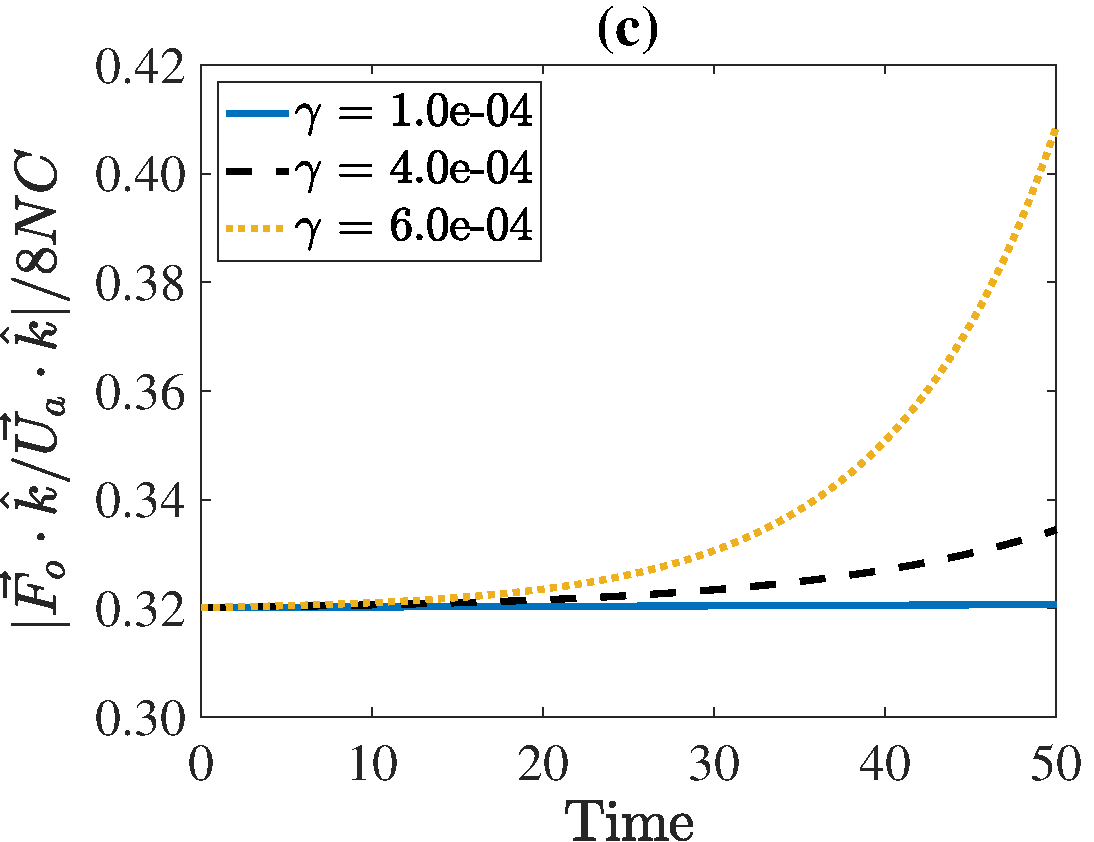
\includegraphics[scale=0.35]{./figures/fig_NC50_g_Fo3Ua_ratio}
		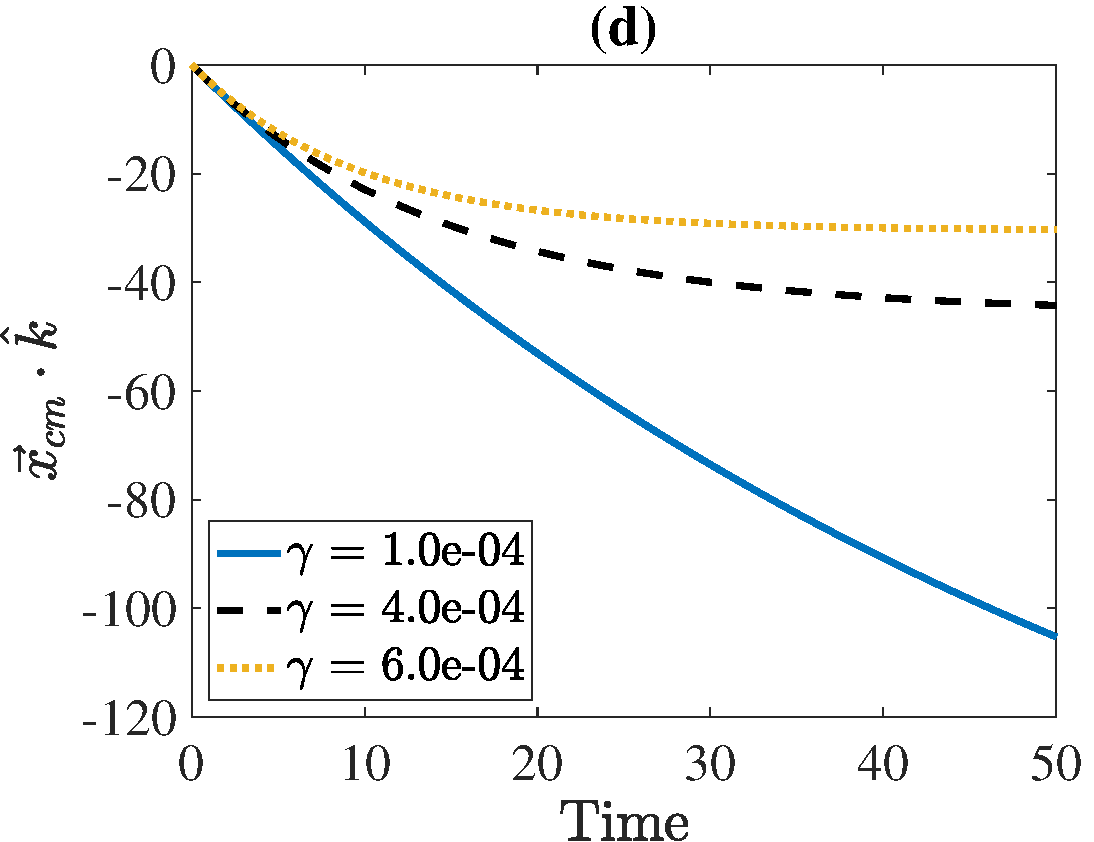
\includegraphics[scale=0.35]{./figures/fig_NC50_g_cm3_all}
	\caption{Compare various background density stratification strengths. We show (a) the settling speed, (b) the vertical force on the aggregate, (c) the ratio of (b) to (a) values, and (d) the position of the center of mass }
	\label{fig_NC50_gg}
\end{center}
\end{figure}
\begin{figure}[h]
	\begin{center}
		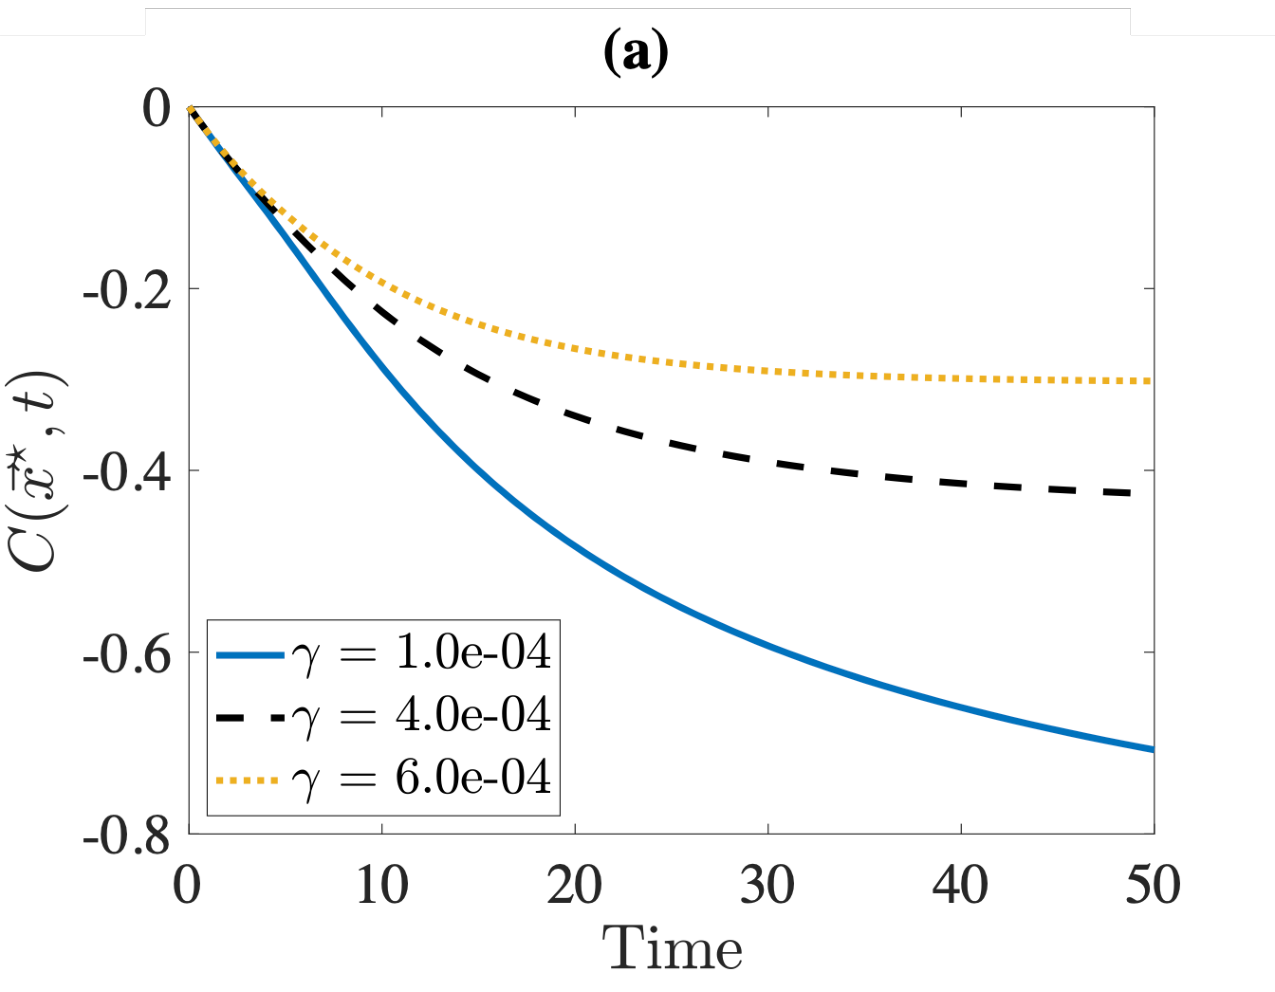
\includegraphics[scale=0.33]{./figures/fig_NC50_g_C_star.pdf}
		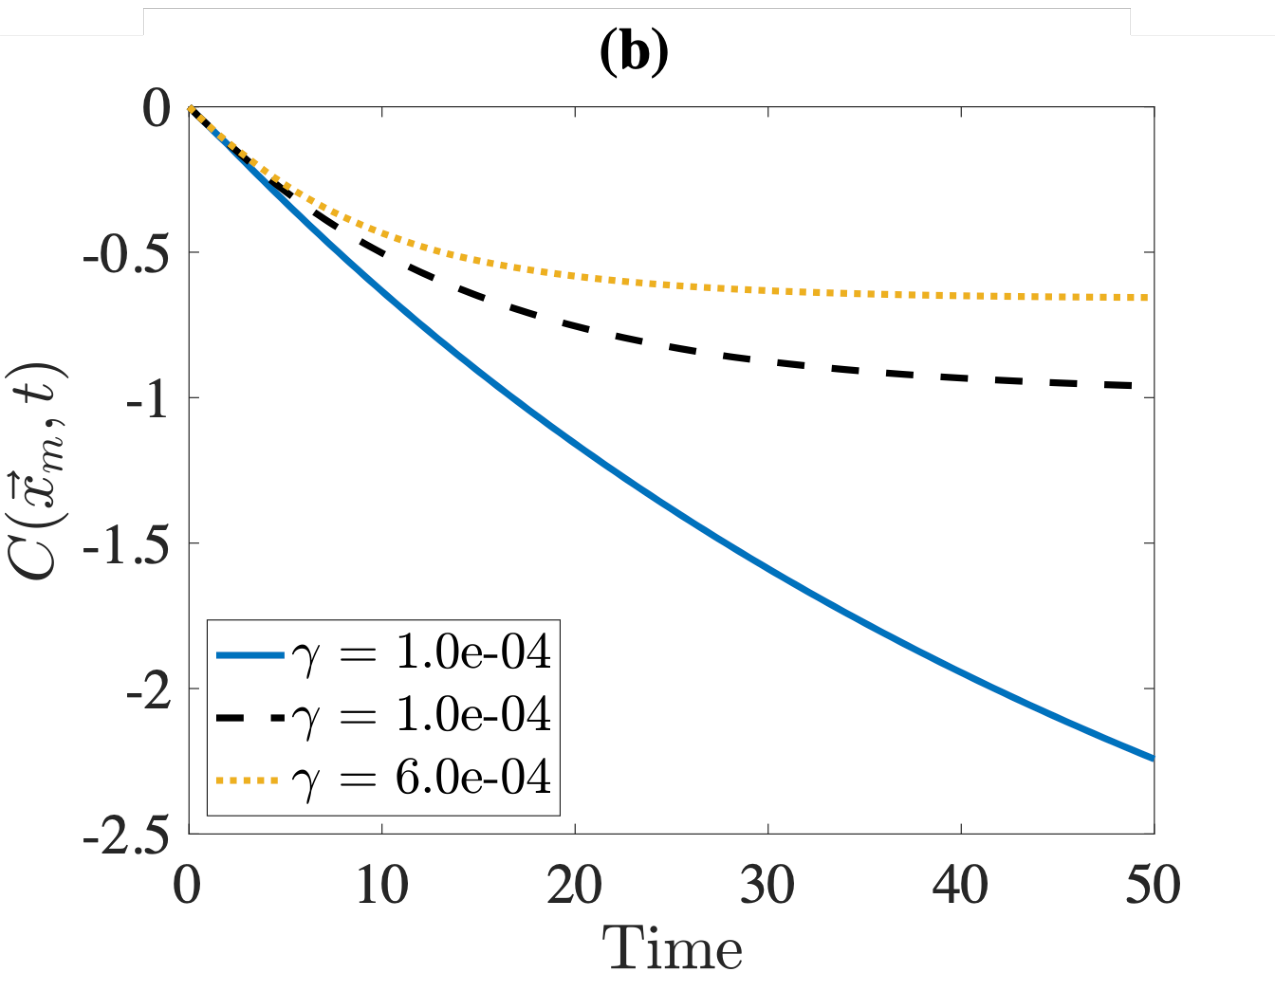
\includegraphics[scale=0.33]{./figures/fig_NC50_g_C_M}
	\caption{Perturbation with various $\gamma$ at (a) the star position $\vec{x}^{\star}$, outside the aggregate, and (b) the center of the fluid domain, inside the aggregate.}
	\label{fig_NC50_gCM}
\end{center}
\end{figure}
\par
We first present quantities of interest 
the aggregate itself in Figure~\ref{fig_NC50_Seeds}. In plot (a), we see that the settling speed of the same aggregate would drop faster when the fluid density gradient gets sharper. Similar results are shown for the total drag over time in plot (b). To clarify, we find the ratio of the drag to the settling speed in plot (c). We observe very similar behavior as a homogeneous fluid case with the smallest $\gamma = 10^{-4}$. Note that this $\gamma$ is considered a small value for the aggregate radius $R_a \approx 9$. For instance, the same $\gamma$ may be a large enough value to observe a clear background fluid stratification effect for an aggregate radius 20.
We also look at the center of mass of aggregate over time. Since $\gamma = 10^{-4}$ mimics a homogeneous fluid, the aggregate travels more, yet with a slower speed, demonstrated by the blue solid line in plot (d).
\par
From a fluid perspective, we obtain the perturbation over time at two different points. In Figure~\ref{fig_NC50_gCM}, the left plot is the perturbation at the usual point, $\vec{x}^{\star}$, where the white star is located in Figure~\ref{fig_NC50_snaps_all}. It is located outside of the aggregate, yet very close. On the right side, we examine the perturbation inside of the aggregate, particularly at the center of the fluid domain. By looking at the magnitude of $C$, there are certainly higher perturbations for all three $\gamma$ cases. Moreover, the perturbation varying range is quite large for the light stratification case (blue line). As we mentioned, it is because the same aggregate stops moving in a stronger density-stratified fluid due to reaching neutral buoyancy.
\section{Conclusion}
As an extension of our study of the homogeneous system~\cite{yoo_hydrodynamic_2020}, we have developed a numerical method to simulate a settling marine aggregate, randomly formed with cubes, using a boundary integral method in a density-stratified fluid.
Applying the net force equilibrium in a Stokes regime, we prescribed the total drag and torque to solve for the stress on the aggregate and its settling velocity using the single-layer potential formula.
With the velocity field obtained, we advance the perturbation in time using the advection-diffusion equation. 
To accelerate the evaluation of integrals of Stokeslet, we incorporate the Fast Multipole Method by modifying the Laplace kernel.
\par
We have validated our methods by providing results of a settling aggregate composed of 10 cubes while varying the spatial grid, time steps, and domain sizes. 
Most of the errors for each comparison appeared to be much smaller than those resulting from assuming that the stress is uniform on each square face of a cube.
\par
Furthermore, we simulated larger aggregates, made with 50 cubes, in different settings. We have observed aggregate settling behavior before its density matches the surrounding fluid density.
We found a consistent trend in the settling behaviors between different shapes of aggregates with, for example, variations in the drag coefficient of the order of 8\%.   
In future work, we can simulate aggregates with more cubes and consider more different shapes for better statistical results. kk
Under the different Péclet number environments, we find the main changes in the perturbation, as expected, between Pe = 1 and Pe = 10. Since a smaller Péclet number implies a higher diffusivity, the perturbation near the aggregate slows down 10\% faster than the other two cases. 
\par
We also explore various stratification strengths via $\gamma$ values. 
Marine aggregates are highly porous and sensitive to surrounding fluid density stratification~\cite{prairie_delayed_2013}. Our results also support these characteristics while we perform the simulations with three types of background fluid density gradients.
In addition to our results in this thesis, potential future work includes considering another applicable regime with different parameters.
\par
We note that a description of rotational flow results is missing, although we have allowed a rotation of an aggregate while obtaining all the numerical results. In short, we have found an approximate torque having the order $\mathcal{O}(10^{-4})$. This is quite a small value compared to the drag force and perturbation effects as a response to the background fluid stratification. 
We consider analyzing more details as future work.
\par
There are several branches we can extend our research further with our comprehensive numerical tools developed. As much research work has been done with a sphere model as an aggregate, we would like to compare our results, such as the settling speed, drag acting on the aggregate, and the amount of concentration entrained. 


